% -*- Mode:TeX -*-

%% The documentclass options along with the pagestyle can be used to generate
%% a technical report, a draft copy, or a regular thesis.  You may need to
%% re-specify the pagestyle after you \include  cover.tex.  For more
%% information, see the first few lines of mitthesis.cls. 

\documentclass[12pt,vi,twoside]{mitthesis}
%%
%%  If you want your thesis copyright to you instead of MIT, use the
%%  ``vi'' option, as above.
%%
%\documentclass[12pt,twoside,leftblank]{mitthesis}
%%
%% If you want blank pages before new chapters to be labelled ``This
%% Page Intentionally Left Blank'', use the ``leftblank'' option, as
%% above. 

%\documentclass[12pt]{mitthesis}
%\documentclass[12pt,singlespace,twoside]{mitthesis}
%\documentclass[12pt,twoside]{mitthesis}
%\documentclass[12pt,oneside]{mitthesis}
%\usepackage{lgrind}
\usepackage{url}
\usepackage{textcomp}
\usepackage{verbatim}
\usepackage{amsmath}
% \usepackage{amsfonts}
% \usepackage{amssymb}    % if you want extra symbols
\usepackage{nicefrac}
\usepackage{mathrsfs}
\usepackage{program}
\usepackage{newlfont}
\usepackage{rotating}
\usepackage{varioref}
\usepackage{graphicx}
\usepackage{subfloat}
%\usepackage{txfont}
\usepackage{makeidx}
%\usepackage{tocbibind}
\usepackage{program}
\usepackage{import}
\usepackage{subfigure}
\usepackage{verbatim}
\usepackage{colortbl}
\usepackage{morefloats}
\usepackage[french,english]{babel}

% \usepackage[LY1]{fontenc}
% \usepackage{patchcmd}
% \usepackage{myfss}
% \usepackage{caslon}
\usepackage{MnSymbol}
\usepackage[mathlf,textlf,minionint]{MinionPro}
\usepackage[T1]{fontenc}
\usepackage{textcomp}

% \renewcommand{\encodingdefault}{LY1}
% \rmshape \rgshape

% \usepackage[oldstyle]{agaramond}
%\usepackage[lining]{agaramond}
% \usepackage[small]{eulervm}
% \usepackage{courier} % for texttt



% \usepackage{ulem} %underlines
% \normalem % normal emph w/ ulem

\usepackage[numbers,square,sort&compress,sectionbib]{natbib}
\usepackage{chapterbib}
\usepackage[pdftex,plainpages=false,breaklinks=true,colorlinks=true,urlcolor=blue,citecolor=blue, linkcolor=blue,bookmarks=true,bookmarksopen=true,bookmarksopenlevel=0,pdfstartview=Fit,pdfview=Fit,pagebackref,linktocpage=true,bookmarksnumbered=true]{hyperref}
\usepackage{hypernat}
\usepackage{array}
\usepackage{supertabular}
\usepackage{booktabs}
\usepackage{placeins}

%%% stuff for doxygen
%\usepackage{times}
\usepackage{multicol}
\usepackage{multirow}
\usepackage{float}
\usepackage{alltt}
\graphicspath{{Figures/}}
% \usepackage{Body/appb/doxygen}
%%%%%%%%%%%

\usepackage{fancyhdr}
%\renewcommand{\chaptermark}[1]{\markboth{\textit{\chaptername}\ \thechapter.\ #1}{}}

\newcommand\blfootnote[1]{%
  \begingroup
  \renewcommand\thefootnote{}\footnote{#1}%
  \addtocounter{footnote}{-1}%
  \endgroup
}

% Declare argmin as a math operator
\DeclareMathOperator*{\argmin}{arg\,min}

%this defines the basic headers and footer
% styles when we use the 'fancyhdr' styles
%\lhead[\fancyplain{}{\itshape\footnotesize\thepage}]{\fancyplain{}{\itshape\footnotesize\rightmark}}
%\rhead[\fancyplain{}{\itshape\footnotesize\leftmark}]{\fancyplain{}{\itshape\footnotesize\thepage}}
%\lhead[\fancyplain{}\bfseries\thepage]{\fancyplain{}\bfseries\rightmark}
%\rhead[\fancyplain{}\bfseries\leftmark]{\fancyplain{}\bfseries\thepage}
%\pagestyle{fancyplain}
\addtolength{\headwidth}{0.5\marginparsep}
\addtolength{\headwidth}{0.5\marginparwidth}
%\renewcommand{\chaptermark}[1]{\markboth{#1}{}}
%\renewcommand{\sectionmark}[1]{\markright{\thesection\ #1}}
\lhead[\fancyplain{}{\footnotesize\thepage}]{\fancyplain{}{\footnotesize\rightmark}}
\rhead[\fancyplain{}{\footnotesize\leftmark}]{\fancyplain{}{\footnotesize\thepage}}
\cfoot{}
\cfoot{}

% Special Float captions
% Different font in captions
\newcommand{\captionfonts}{\mdseries}
\newcommand{\floatnamefonts}{\bfseries}
\makeatletter  % Allow the use of @ in command names
\long\def\@makecaption#1#2{%
  \vskip\abovecaptionskip
  \sbox\@tempboxa{{\floatnamefonts #1:~~\captionfonts #2}}%
  \ifdim \wd\@tempboxa >\hsize
    {\floatnamefonts #1: \captionfonts #2\par}
  \else
    \hbox to\hsize{\hfil\box\@tempboxa\hfil}%
  \fi
  \vskip\belowcaptionskip}
\makeatother   % Cancel the effect of \makeatletter

\makeindex

\pagestyle{plain}

%% This bit allows you to either specify only the files which you wish to
%% process, or `all' to process all files which you \include.
%% Krishna Sethuraman (1990).

\begin{document}
% \fontencoding{LY1}\fontfamily{ACaslonPro}\mdweight

% -*-latex-*-
% $Log: cover.tex,v $
% Revision 1.7  2001/02/08 18:53:16  boojum
% changed some \newpages to \cleardoublepages
%
% Revision 1.6  1999/10/21 14:49:31  boojum
% changed comment referring to documentstyle
%
% Revision 1.5  1999/10/21 14:39:04  boojum
% *** empty log message ***
%
% Revision 1.4  1997/04/18  17:54:10  othomas
% added page numbers on abstract and cover, and made 1 abstract
% page the default rather than 2.  (anne hunter tells me this
% is the new institute standard.)
%
% Revision 1.4  1997/04/18  17:54:10  othomas
% added page numbers on abstract and cover, and made 1 abstract
% page the default rather than 2.  (anne hunter tells me this
% is the new institute standard.)
%
% Revision 1.3  93/05/17  17:06:29  starflt
% Added acknowledgements section (suggested by tompalka)
% 
% Revision 1.2  92/04/22  13:13:13  epeisach
% Fixes for 1991 course 6 requirements
% Phrase "and to grant others the right to do so" has been added to 
% permission clause
% Second copy of abstract is not counted as separate pages so numbering works
% out
% 
% Revision 1.1  92/04/22  13:08:20  epeisach
\addcontentsline{toc}{chapter}{Cover page}
\title{Quantification of Tissue Perfusion using Contrast-Enhanced Ultrasound: 
Toward Robust Exam Comparison}
\author{Maxime Doury}
\department{Laboratoire d'Imagerie Biom\'edicale}
% If the thesis is for two degrees simultaneously, list them both
% separated by \and like this:
 \degree{Doctor of Physics}
%\degree{Bachelor of Science in Computer Science and Engineering}
\degreemonth{September}
\degreeyear{2017}
\thesisdate{September 29, 2017}

%% By default, the thesis will be copyrighted to MIT.  If you need to copyright
%% the thesis to yourself, just specify the `vi' documentclass option.  If for
%% some reason you want to exactly specify the copyright notice text, you can
%% use the \copyrightnoticetext command.  
% \copyrightnoticetext{\copyright ~Maxime Doury, 2017.}

\copyrightnoticetext{\copyright ~Maxime Doury, 2017. \\
{\footnotesize
This work is licensed under the Creative
Commons Attribution-NonCommercial 4.0
License. To view a copy of this license, visit
\url{http://creativecommons.org/licenses/by-nc/4.0} or send a
letter to
Creative Commons
543 Howard Street, 5th Floor,
San Francisco, California, 94105, USA.
}}

% If there is more than one supervisor, use the \supervisor command
% once for each.
\supervisor{Fr\'ed\'erique Frouin}{IMIV, Inserm, Paris Sud}
\supervisor{Alain de Cesare}{LIB, CNRS, UPMC}

% This is the department committee chairman, not the thesis committee
% chairman.  You should replace this with your Department's Committee
% Chairman.
%\chairman{Daniel Blankschtein}{Chairman, Department Committee on Graduate Students}
\chairman{William M. Deen}{Chairman, Department Committee on Graduate Students}

% Make the titlepage based on the above information.  If you need
% something special and can't use the standard form, you can specify
% the exact text of the titlepage yourself.  Put it in a titlepage
% environment and leave blank lines where you want vertical space.
% The spaces will be adjusted to fill the entire page.  The dotted
% lines for the signatures are made with the \signature command.
\maketitle

% The abstractpage environment sets up everything on the page except
% the text itself.  The title and other header material are put at the
% top of the page, and the supervisors are listed at the bottom.  A
% new page is begun both before and after.  Of course, an abstract may
% be more than one page itself.  If you need more control over the
% format of the page, you can use the abstract environment, which puts
% the word "Abstract" at the beginning and single spaces its text.

%% You can either \input (*not* \include) your abstract file, or you can put
%% the text of the abstract directly between the \begin{abstractpage} and
%% \end{abstractpage} commands.

% First copy: start a new page, and save the page number.
\cleardoublepage
% Uncomment the next line if you do NOT want a page number on your
% abstract and acknowledgments pages.
\pagestyle{empty}
% \setcounter{savepage}{\thepage}
\begin{abstractpage}\addcontentsline{toc}{chapter}{Abstract}
% $Log: abstract.tex,v $
% Revision 1.1  93/05/14  14:56:25  starflt
% Initial revision
%
% Revision 1.1  90/05/04  10:41:01  lwvanels
% Initial revision
%
%
%% The text of your abstract and nothing else (other than comments) goes here.
%% It will be single-spaced and the rest of the text that is supposed to go on
%% the abstract page will be generated by the abstractpage environment.  This
%% file should be \input (not \include 'd) from cover.tex.
In this thesis, I discuss the application and development of methods
for the automated discovery of motifs in sequential data.  These data
include DNA sequences, protein sequences, and real--valued
sequential data such as protein structures and timeseries of
arbitrary dimension. As more genomes are sequenced and annotated,
the need for automated, computational methods for analyzing
biological data is increasing rapidly.  In broad terms, the goal of
this thesis is to treat sequential data sets as unknown languages
and to develop tools for interpreting an understanding these
languages.

The first chapter of this thesis is an introduction to the
fundamentals of motif discovery, which establishes a common mode of
thought and vocabulary for the subsequent chapters.  One of the
central themes of this work is the use of grammatical models,
which are more commonly associated with the field of computational
linguistics.  In the second chapter, I use grammatical models to
design novel antimicrobial peptides (AmPs). AmPs are small proteins
used by the innate immune system to combat bacterial infection in
multicellular eukaryotes. There is mounting evidence that these
peptides are less susceptible to bacterial resistance than
traditional antibiotics and may form the basis for a novel class of
therapeutics. In this thesis, I described the rational design of
novel AmPs that show limited homology to naturally--occurring
proteins but have strong bacteriostatic activity against several
species of bacteria, including \emph{Staphylococcus aureus} and
\emph{Bacillus anthracis}. These peptides were designed using a
linguistic model of natural AmPs by treating the amino acid
sequences of natural AmPs as a formal language and building a set of
regular grammars to describe this language. This set of grammars was
used to create novel, unnatural AmP sequences that conform to the
formal syntax of natural antimicrobial peptides but populate a
previously unexplored region of protein sequence space.

The third chapter describes a novel, GEneric MOtif DIscovery
Algorithm (Gemoda) for sequential data. Gemoda can be applied to any
dataset with a sequential character, including both categorical and
real--valued data.  As I show, Gemoda deterministically discovers
motifs that are maximal in composition and length.  As well, the
algorithm allows any choice of similarity metric for finding motifs.
These motifs are representation--agnostic: they can be represented
using regular expressions, position weight matrices, or 
any other model for sequential data. I demonstrate a
number of applications of the algorithm, including the discovery of
motifs in amino acids and DNA sequences, and the discovery of
conserved protein sub--structures.

The final chapter is devoted to a series of smaller projects,
employing tools and methods indirectly related to motif discovery in
sequential data.  I describe the construction of a software tool,
Biogrep that is designed to match large pattern sets against large
biosequence databases in a \emph{parallel} fashion. This makes
biogrep well--suited to annotating sets of sequences using
biologically significant patterns.  In addition, I show that the
BLOSUM series of amino acid substitution matrices, which are
commonly used in motif discovery and sequence alignment problems,
have changed drastically over time.  The fidelity of amino acid
sequence alignment and motif discovery tools depends strongly on the
target frequencies implied by these underlying matrices.  Thus,
these results suggest that further optimization of these matrices is
possible.

The final chapter also contains two projects wherein I apply
statistical motif discovery tools instead of grammatical tools. In
the first of these two, I develop three different physiochemical
representations for a set of roughly 700 HIV--I protease substrates
and use these representations for sequence classification and
annotation.  In the second of these two projects, I develop a simple
statistical method for parsing out the phenotypic contribution of a
single mutation from libraries of functional diversity that contain
a multitude of mutations and varied phenotypes.  I show that this
new method successfully elucidates the effects of single nucleotide
polymorphisms on the strength of a promoter placed upstream of a
reporter gene.

The central theme, present throughout this work, is the development
and application of novel approaches to finding motifs in sequential
data.  The work on the design of AmPs is very applied and relies
heavily on existing literature.  In contrast, the work on Gemoda is
the greatest contribution of this thesis and contains many new
ideas.

\end{abstractpage}

% Additional copy: start a new page, and reset the page number.  This way,
% the second copy of the abstract is not counted as separate pages.
% Uncomment the next 6 lines if you need two copies of the abstract
% page.
% \setcounter{page}{\thesavepage}
% \begin{abstractpage}
% % $Log: abstract.tex,v $
% Revision 1.1  93/05/14  14:56:25  starflt
% Initial revision
%
% Revision 1.1  90/05/04  10:41:01  lwvanels
% Initial revision
%
%
%% The text of your abstract and nothing else (other than comments) goes here.
%% It will be single-spaced and the rest of the text that is supposed to go on
%% the abstract page will be generated by the abstractpage environment.  This
%% file should be \input (not \include 'd) from cover.tex.
In this thesis, I discuss the application and development of methods
for the automated discovery of motifs in sequential data.  These data
include DNA sequences, protein sequences, and real--valued
sequential data such as protein structures and timeseries of
arbitrary dimension. As more genomes are sequenced and annotated,
the need for automated, computational methods for analyzing
biological data is increasing rapidly.  In broad terms, the goal of
this thesis is to treat sequential data sets as unknown languages
and to develop tools for interpreting an understanding these
languages.

The first chapter of this thesis is an introduction to the
fundamentals of motif discovery, which establishes a common mode of
thought and vocabulary for the subsequent chapters.  One of the
central themes of this work is the use of grammatical models,
which are more commonly associated with the field of computational
linguistics.  In the second chapter, I use grammatical models to
design novel antimicrobial peptides (AmPs). AmPs are small proteins
used by the innate immune system to combat bacterial infection in
multicellular eukaryotes. There is mounting evidence that these
peptides are less susceptible to bacterial resistance than
traditional antibiotics and may form the basis for a novel class of
therapeutics. In this thesis, I described the rational design of
novel AmPs that show limited homology to naturally--occurring
proteins but have strong bacteriostatic activity against several
species of bacteria, including \emph{Staphylococcus aureus} and
\emph{Bacillus anthracis}. These peptides were designed using a
linguistic model of natural AmPs by treating the amino acid
sequences of natural AmPs as a formal language and building a set of
regular grammars to describe this language. This set of grammars was
used to create novel, unnatural AmP sequences that conform to the
formal syntax of natural antimicrobial peptides but populate a
previously unexplored region of protein sequence space.

The third chapter describes a novel, GEneric MOtif DIscovery
Algorithm (Gemoda) for sequential data. Gemoda can be applied to any
dataset with a sequential character, including both categorical and
real--valued data.  As I show, Gemoda deterministically discovers
motifs that are maximal in composition and length.  As well, the
algorithm allows any choice of similarity metric for finding motifs.
These motifs are representation--agnostic: they can be represented
using regular expressions, position weight matrices, or 
any other model for sequential data. I demonstrate a
number of applications of the algorithm, including the discovery of
motifs in amino acids and DNA sequences, and the discovery of
conserved protein sub--structures.

The final chapter is devoted to a series of smaller projects,
employing tools and methods indirectly related to motif discovery in
sequential data.  I describe the construction of a software tool,
Biogrep that is designed to match large pattern sets against large
biosequence databases in a \emph{parallel} fashion. This makes
biogrep well--suited to annotating sets of sequences using
biologically significant patterns.  In addition, I show that the
BLOSUM series of amino acid substitution matrices, which are
commonly used in motif discovery and sequence alignment problems,
have changed drastically over time.  The fidelity of amino acid
sequence alignment and motif discovery tools depends strongly on the
target frequencies implied by these underlying matrices.  Thus,
these results suggest that further optimization of these matrices is
possible.

The final chapter also contains two projects wherein I apply
statistical motif discovery tools instead of grammatical tools. In
the first of these two, I develop three different physiochemical
representations for a set of roughly 700 HIV--I protease substrates
and use these representations for sequence classification and
annotation.  In the second of these two projects, I develop a simple
statistical method for parsing out the phenotypic contribution of a
single mutation from libraries of functional diversity that contain
a multitude of mutations and varied phenotypes.  I show that this
new method successfully elucidates the effects of single nucleotide
polymorphisms on the strength of a promoter placed upstream of a
reporter gene.

The central theme, present throughout this work, is the development
and application of novel approaches to finding motifs in sequential
data.  The work on the design of AmPs is very applied and relies
heavily on existing literature.  In contrast, the work on Gemoda is
the greatest contribution of this thesis and contains many new
ideas.

% \end{abstractpage}

\cleardoublepage

\section*{Acknowledgments}\addcontentsline{toc}{chapter}{Acknowledgments}


I am indebted to many people who both directly and indirectly
contributed to this thesis.  First, I would like to thank those
collaborators who directly contributed.  Most of all, I'm grateful
for the help and friendship of Mark Styczynski. Mark was my
collaborator on all matters computational for the past four years
--- his influence is evident throughout this document.  I'm also
grateful for my collaboration with Christopher Loose, who performed
many of the experiments on antimicrobial peptides described in
Chapter~\ref{chapter:amps}.  Finally, I would like to thank Isidore Rigoutsos, who
straddled the line between collaborator and advisor.  Isidore taught
me an attention to detail and a penchant for the UNIX command line
and vi editor.

Most importantly, I am indebted to Greg Stephanopoulos, my advisor,
whose guidance and support was unwavering these past six years. Greg
is the perpetual optimist --- always positive in the face of my many
failures along the way.  He also gave me the freedom to pursue
projects of my own choosing, which contributed greatly to my
academic independence, if not the selection of wise projects.

I am much obliged to my thesis committee members: my advisor Greg,
Isidore, Bill Green, and Bob Berwick.  My committee was always
flexible in scheduling and judicious in their application of both
carrots and sticks.

There are numerous people who contributed indirectly to this thesis.
First among these is my intelligent, lovely, and vivacious wife
Kathryn Miller--Jensen.  Next, my parents Carl and Julie, my sister
Heather, and my in-laws, Ron, Joyce, Suzanne, Jeff, and Mindi.
Finally, there are innumerable friends who contributed and to whom I
am greatly appreciative including Michael Raab, Joel Moxley, Bill
Schmitt, Vipin Guptda, and Jatin Misra.


%%%%%%%%%%%%%%%%%%%%%%%%%%%%%%%%%%%%%%%%%%%%%%%%%%%%%%%%%%%%%%%%%%%%%%
% -*-latex-*-

\pagestyle{plain}
% -*- Mode:TeX -*-
%% This file simply contains the commands that actually generate the table of
%% contents and lists of figures and tables.  You can omit any or all of
%% these files by simply taking out the appropriate command.  For more
%% information on these files, see appendix C.3.3 of the LaTeX manual. 
\tableofcontents\addcontentsline{toc}{chapter}{Contents}
\newpage
\listoffigures\addcontentsline{toc}{chapter}{List of Figures}
\newpage
\listoftables\addcontentsline{toc}{chapter}{List of Tables}



%now start the fancy headings
\pagestyle{fancyplain}
\addtolength{\headheight}{\baselineskip}
%add a nice little line underneath the heading
\renewcommand{\headrulewidth}{0.6pt}


%!TeX root = ./main.tex
%% This is an example first chapter.  You should put chapter/appendix that you
%% write into a separate file, and add a line \include{yourfilename} to
%% main.tex, where `yourfilename.tex' is the name of the chapter/appendix file.
%% You can process specific files by typing their names in at the 
%% \files=
%% prompt when you run the file main.tex through LaTeX.
% \cleardoublepage
\part*{Introduction}
\chapter{Introduction}\label{chapter:intro}
This thesis addresses the quantification of tumor perfusion using contrast-enhanced ultrasound imaging.
In this chapter, we present the biological and technical context that motivated this thesis.
The research was performed at the {\em Laboratoire d'Imagerie Biom\'edicale} (LIB), and was financed by the {\em Fondation pour la Recherche M\'edicale} (FRM) through grant DBS20131128436.
The global project aims at developing a multiparametric tumor tissue classification tool, based on multiple ultrasound imaging modalities, including quantitative ultrasound, elastosonography, and contrast-enhanced ultrasound.
The data should be used to develop a realistic tumor growth model, as well as an appropriate treatment response prediction model.
The first step of this project was therefore the accurate estimation of parameters from ultrasound data in order to obtain reproducible results and use them in longitudinal studies.

\section{Cancer and tumor microenvironment}
\label{sec:IntroCancer}
A tumor is a neoplasm composed of mutated cells undergoing abnormal growth.
All tumors are not cancers, in particular benign tumors are not cancers, they are not invasive and usually not life-thretening.
Cancer is in fact synonym of malignant tumor.

In \citeyear{Hanahan:2000hx}, \citet{Hanahan:2000hx} proposed the first generation of cancer hallmarks, i.e.~six acquired traits that differentiate cancerous cells from benign tumors and normal tissues:
\begin{enumerate}
    \item Cancerous cells are able to generate their own mitogenic growth signals, and do not rely on the growth signals from the surrounding environment.
    \item Cancerous cells are insensitive to the anti-growth signals originating from the surrounding environment.
    \item Cancerous cells are immune to apoptotic signals, emitted by the environment, and controlling the death of malfunctionning cells.
    \item The number of replication cancerous cells can achieve is unlimited.
    \item After cancerous cells reached a point where further proliferation is limited by the supply in oxygen and nutrients, they switch to an angiogenic state that triggers the construction of a supplying vascular network, allowing rapid cell proliferation despite its chaotic structure.
    \item When nutrients and space become limiting growth factors, cancerous cells are able to migrate and invade surrounding tissues where nutrients and space are not limiting factors to create new cancerous cell colonies known as metastases.
\end{enumerate}

Later, in \citeyear{Hanahan:2011gu}, \citet{Hanahan:2011gu} proposed a second generation of cancer hallmarks that include the six acquired traits presented in the previous paragraph, but they add four more hallmarks:
\begin{enumerate}
    \item Cancerous cells are able to modify their metabolism to most effectively support tumor proliferation.
    \item Cancerous cells are resistant to immunological destruction by lymphocytes and macrophages.
    \item Cancerous cells exhibit unstable genomes favoring genetic mutations, that often result in an accelerated tumor progression.
    \item Immune cells fighting the proliferation of cancer cells cause tissue inflammation, which can contribute to the acquired traits presented in their first paper.
\end{enumerate}

\paragraph{Treatment of cancer}
\label{sec:IntroCancerTreatment}
The three major treatments of cancer are surgery, radiotherapy, and chemotherapy.

Surgery aims at removing the whole tumor, however this procedure is highly invasive.
Radiotherapy consists in the irradiation of the tumor by high-energy X-rays, gamma-rays or charged particles, damaging cancerous cells, but also the surrounding tissues. 
These two techniques are only applicable to localized solid tumors, and some cancerous cells can remain after the treatment.

If the cancer has spread throughout the body, chemotherapy is often used to eliminate remaining and migrating cells after removal of the primary tumor by means of surgery or radiotherapy.
Chemotherapy relies on the injection of a cytotoxic agent, which main purpose is to eradicate the remaining cancerous cells.
Cytotoxic agents however, are not specific of cancerous cells and are globally toxic for the patient, limiting the injected doses.
Moreover, since cancerous cells are highly prone to mutations, they can develop a resistance to the cytotoxic agent.

Recently, anti-angiogenic treatments were proposed to disrupt or to limit the development of new vascular structures providing the tumor with the oxygen and nutrients necessary for cell division, therefore limiting further growth of the tumor. 
These treatments were shown to normalize the chaotic neovascularization in tumors, allowing a more efficient delivery of cytotoxic therapies inside the tumor. % REF
However, since many pathways regulating angiogenesis exist, cancerous cells can bypass the targeted pathway and activate another one, making the tumor resistant to the anti-angiogenic treatment.

\paragraph{Cancer monitoring}
Surgery, radiotherapy, and chemotherapy directly target cancerous cells, and an efficient treatment should have a direct impact on the size of the tumor.
Therefore, morphological criteria were proposed to assess tumor response to therapy.
The classical RECIST and WHO criteria are based on the changes in tumor diameter, and give an indication on the evolution of the disease, i.e.~stable, regressive, or progressive.

Oppositely, anti-angiogenic treatments do not target cancerous cells, but rather the neovascularization of the tumor.
They do not have a direct impact on the size of the tumor, especially at the early stages of the treatment.
Therefore, classical morphological criteria fail to reveal the efficiency of such treatments.
Quantification of tumor angiogenesis and of the response to anti-angiogenic treatments requires the development of functional criteria assessing the microvascularization of tumor tissues.
Microvascularization can be observed in vivo using functional imaging, and in particular through perfusion imaging.

\section{Perfusion imaging}
\label{sec:IntroPerfusionImaging}
Perfusion imaging is a branch of medical imaging that focuses on the visualization and characterization of tissue vascularization.
A tracer or contrast-agent is injected intravascularly, either as a bolus or as an infusion, and the passage of the tracer in the tissue is observed using one of the various imaging modalities presented below.
Indeed, despite the various physical phenomena involved during image acquisition in the various contrast-enhanced imaging modalities, analysis of the passage of the contrast agent follows the same general principle.

\paragraph{Nuclear medicine}
\label{sec:IntroNM}
Nuclear medicine regroups imaging modalities using radioactive tracers. 
Planar scintigraphy uses gamma-emitting tracers and a single gamma camera, yielding projections images of the tracer concentration.
Single-photon emission computed tomography (SPECT) uses the same tracers as scintigraphy, but uses a rotating gamma camera to create three-dimensional volumes of the tracer concentration.
Positron emission tomography (PET) uses a positron-emitting tracer, and a coincident detection of the two gamma rays resulting from the annihilation of the positron emitted during the beta decay of the radioactive isotope.

Radioactive isotopes are usually attached to a biological molecule, forming a radiotracer that follows the distribution of the biological molecule and enables its tracking in miological systems.

\paragraph{X-ray computed tomography (CT)}
\label{sec:IntroCT}
X-ray computed tomography uses a combination of multiple planar X-ray projections with varying angles to produce three-dimensional images, the resulting volumes show the absorption of X-rays. 
The contrast agents used for X-ray computed tomography are usually iodinated compounds that were chosen for their high radiodensity, resulting in a strong absorption of the X-ray beams, and for their fast renal elimination.
Additionally, they exhibit a linear relation between the X-ray attenuation and the concentration of contrast-agent.

\paragraph{Magnetic resonance imaging (MRI)}
\label{sec:IntroMR}
MRI is based on nuclear magnetic resonance that exploits the ability of some atoms to absorb and emit radio frequencies when placed in an external magnetic field.
Typically, the imaged nuclides are protons present in tissues composed of water molecules.
In this case, magnetic resonance images are formed by measuring the spin-lattice (T1) and spin-spin (T2) relaxation times of the protons inside the studied tissue.

Magnetic resonance contrast agents are usually paramagnetic substances that shorten the T1 relaxation time of the protons inside the observed tissues, for instance Gadolinium chelates are widely used.
Most Gadolinium-based contrast agents diffuse from the blood pool to the interstitial space through the capillary surface.
However intravascular contrast agents were also developed for magnetic resonance imaging, but their usage is mainly restricted to research.
Endogenous tracers are also being developed for MRI, for instance arterial spin labelling (ASL) allows tracking of spin-labelled arterial blood and alleviates the need for injection of a exogenous contrast agent.

\paragraph{Contrast-enhanced ultrasound (CEUS)}
\label{sec:IntroCEUS}
Ultrasound images are formed by sending sequences of ultrasound pulses inside the tissue using a transducer, the ultrasound pulses are reflected by scatterers in the tissue, and the reflected pulses are then recorded by the transducer.
The recorded signals are processed to retrieve the time of flight of the echo, determining the location of the scatterer in the image, as well as the strength of the echo, determining the image intensity associated to the scatterer.

Coated gas-filled microbubbles are used as ultrasound contrast agents for their ability to oscillate asymetrically when exposed to acoustic waves, and for their size that makes them resonate in the ultrasound frequency domain~\cite{Greis:2004ub}.
Their size being nearly the same as the size of a red blood cell, they can go everywhere in the vascular system, from the largest arteries to the smallest capillaries, and they do not leak in the interstitial space.
Microbubbles exhibit a strong and specific non-linear response to ultrasound pulses.
This non-linearity is exploited by ultrasound scanners using specific background-cancelling sequences to produce contrast-specific images, e.g.~harmonic imaging~\cite{Meairs:2000eq}, subharmonic imaging~\cite{Eisenbrey:2015gk}, contrast pulse sequencing (CPS)~\cite{Phillips:2004ke}.

Microbubbles can be disrupted using ultrasound pulses with high mechanical indices~\cite{Tiemann:1999vy}.
This phenomenon allows a type of acquisition specific of contrast-enhanced ultrasound in addition to conventional approaches. 
Indeed, after a continuous infusion of microbubbles reached its steady-state, a series of disruptive pulses is sent, then the refillment of the microbubbles in the tissue is observed in real-time using a low mechanical contrast-specific sequence to ensure minimum destruction of the microbubbles.

Indeed, the spatial resolution of contrast-enhanced ultrasound images depends on the central frequency of the ultrasound probe, but is usually of about 100~$\mu$m.
The spatial resolution of nuclear medicine images is generally much coarser, for instance the resolution of PET images is typically about 0.5~cm.
Additionally, ultrasound images can be acquired at high frame rates, i.e.~ranging from 1~Hz to more than 1~kHz using plane wave imaging.
These fine temporal resolutions can however be obtained without sacrificing the image spatial resolution or quality. 
This is for instance not true in MRI where a compromise must be made between the temporal resolution, the spatial resolution, and the signal to noise ratio.

Contrast-enhanced ultrasound is a non-ionizing imaging modalities, enabling repeated acquisitions without exposing the patient to radiations.
This is especially important in pathology monitoring and treatment response monitoring applications.
Contrast-enhanced ultrasound is the only real-time perfusion imaging modality available in clinical routine, allowing direct visualization of the passage of microbubbles in the imaging plane on the scanner terminal, whereas tomographic imaging modalities, i.e.~SPECT, PET, X-ray CT or MRI, usually require offline precessing to generate the dynamic perfusion volume.
Ultrasound scanners are smaller than other imaging apparatuses, most scanners are actually designed to be moved around the patient and are therefore mounted on wheels.
Some miniature scanners, specifically designed for mobility applications, even include batteries for autonomous usage.
Additionally, ultrasound scanners are much cheaper than other imaging apparatus, and do not require expensive or short-lived consumables.

\section{Aims and outline}
\label{sec:IntroAimsOutline}
\subsection{Aims}
Reliable quantification of tumor perfusion is a challenging yet necessary task to establish cancer diagnosis and monitor tumors undergoing therapy.
Contrast-enhanced imaging is a great tool to assess perfusion, however quantitative exam comparison remains difficult because of the poor reproducibility of the acquisitions.
Moreover, most of the perfusion quantification methods are developped to estimate parameters at a global scale, therefore either hiding the local variations in tissue perfusion or not accounting for the relations between the local estimates.
This thesis aims at making the estimation of perfusion parameters robust to inter-exam changes, in order to enable exam comparison while revealing the spatial heterogeneity of the tissue vascular function.
Various quantification approaches will therefore be investigated in this thesis, including semi-quantitative approaches, and compartmental models using either an arterial input function or a reference tissue.
Additionally, various estimation methods and their impact on the estimated parameters will be investigated.
Our study focused on contrast-enhanced ultrasound data, however the proposed quantification methods could be investigated in other perfusion imaging modalities.

\subsection{Outline}
The document is divided into three parts. 
In the first part we establish a state of the art of the methods for quantification of perfusion.
In the second part we assess the reproducibility of existing quantification methods.
And in the third part we propose a new quantification method, and then assess its reproducibility and its sensitivity to various factors.

\paragraph{Part I - Quantification of perfusion: state of the art}
Chapter~\ref{chapter:review} presents a state of the art of the methods that have been proposed for the quantification of perfusion, and in particular using medical imaging.
Quantification approaches are classified into three categories: semi-quantitative, deconvolution-based, or compartmental models.
Indeed, the two last categories consider an arterial input function, and compartmental modeling is a specific case of deconvolution.
Some main studies from the litterature were reviewed, focusing on earlier work at the origin of methodological developments.


\paragraph{Part II - Reproducibility of the existing methods and the relations between them}
Chapter~\ref{chapter:PMB} studies the impact of mathematical modeling on the reproducibility of perfusion parameters through preclinical test-retest experiments.
This study revealed the sensitivity of absolute semi-quantitative parameters to inter-exam variations in experimental or physiological conditions.
It also showed the superiority of of normalized parameters, and more precisely of the reference tissue model, in terms of reproducibility.
Chapter~\ref{chapter:PMB2} extends the work from Chapter~\ref{chapter:PMB} by first establishing theoretically and then verifying experimentally the relations between the parameters of the various models.
The existence of these relations shows the ability of semi-quantitative parameters to reveal relative variations of the vascular function.

\paragraph{Part III - Proposition and assessment of a new quantification method}
Chapter~\ref{chapter:IUS} first presents a new regularized linear estimation method for the reference tissue model, and compares its parameters to those obtained using the classical linear estimation method in terms of reproducibility.
This study proves the superior robustness of the regularized estimates to inter-exam variations.
Then Chapter~\ref{chapter:IRBM} compares the robustness of the two models to contrast-agent recirculation through simulation experiments.
And Chapter~\ref{chapter:PLOSONE} studies the accuracy and the precision of the models when varying intrinsic characteristics of the data, e.g.~exam duration, noise level, or quantification strategies, e.g.~reference tissue, number of regions.

\newpage
\bibliographystyle{plainnat}
\bibliography{Bibliography/chap1}
\part{Quantification of perfusion: state~of~the~art}
%!TeX root = ../main.tex
\chapter{Quantification of perfusion exams: A review}\label{chapter:review}

Generally speaking, quantification of perfusion consists in deriving parameters from blood flow measurements, regardless of the method used for the measure. 
This topic has been on the table, and continuously evolving, long before perfusion imaging existed. 
Indeed, G.N.~Stewart introduced indicator dilution theory, starting with the founding paper published in the Journal of Physiology in 1897~\cite{Stewart:1897dz}. 
W.F.~Hamilton went further, corrected the approximations made by Stewart.
Even before Stewart and Hamilton, hemodynamics of the heart had been studied  through indirect measurements and reported in German language by \citet{Volkmann:1850us} and \citet{Vierordt:82xUDMVI} in the 1850s, and later through direct measurements by \citet{Stolnikow:1886wm} and \citet{Tigerstedt:1891wn}.

This chapter fundamentally aims to review the various methods used to quantify perfusion exams acquired using one of the imaging modality described in Chapter~\ref{sec:IntroPerfusionImaging}. 
Realistically, this review of perfusion quantification techniques cannot be close to comprehensive, instead it tackles the subject from the three angles mentioned thereafter, and emphasis the major landmarks of the perfusion quantification landscape.

Section~\ref{sec:SQMethods} presents semi-quantitative methods, extracting parameters directly either from raw or noise-filtered enhancement curves. 
Then Section~\ref{sec:DeconvolutionMethods} presents deconvolution-based quantification methods, estimating the vascular transfer function in the tissue of interest by means of blind or regularized deconvolution.
Finally, compartmental models accounting for the various interactions of the contrast agent with the tissue are presented in Section~\ref{sec:CompartmentalModels}. 

\section{Semi-quantitative methods}
\label{sec:SQMethods}
\subsection{Generalities}
Semi-quantitative methods are probably among the most intuitive as they extract perfusion-related parameters directly from raw, interpolated, or noise-filtered enhancement curves.
They are however not directly related to any physiological function and are prone to changes in experimental or physiological conditions.
They are therefore often used as relative indicators of perfusion and contrast agent transit time~\cite{Miles:1991et}, allowing intra-exam comparisons.

Examples of semi-quantitative parameters include the peak enhancement~\cite{Norman:1978ji,Nally:1985te,Pettersson:1987ft,Erlemann:1989ib}, the time to peak enhancement~\cite{Norman:1978ji,Erlemann:1989ib,Dietrich:2012kw}, maximum upslope gradient, also known as wash-in rate~\cite{Nally:1985te,Erlemann:1989ib}, the area under the enhancement curve~\cite{Dietrich:2012kw}, but also perfusion parameters based on indicator dilution theory based on the previously cited parameters~\cite{Hilson:1978us,Peters:1987fa,Peters:1987vx,Miles:1991et,Miles:1991ei,Miles:1993cq,Blomley:1995vs,Koenig:1998ir}.
Figure~\ref{fig:SQParameters} shows graphical representations of the above mentioned semi-quantitative parameters. 

\subsection{Nuclear medicine}
\label{sec:SQNM}
Semi-quantitative parameters have been used to differentiate stenosed from healthy kidney in scintigraphy exams, i.e.~a nuclear medicine technique using a gamma camera, following bolus injection of $\left[^{99m}Tc\right]$DTPA.

For instance, Hilson et al.~and later Peters et al.~both proposed an enhancement-based perfusion index, which is commonly defined as the ratio of the tissue blood flow to the cardiac output. 
On the one hand, Hilson et al.~defined the perfusion index as the ratio of the area under the arterial curve to the area under the renal curve, both curves are integrated up to the arterial peak~\cite{Hilson:1978us}.
On the other hand, Peters et al.~defined the perfusion index as the ratio of the maximum upslope of the renal curve normalized for the injected quantity to the maximum upslope of the integrated arterial curve normalized for the area under the arterial enhancement curve, and multiplied by a constant converting the gamma camera into a unit of activity~\cite{Peters:1987fa,Peters:1987vx}. 

Nally et al.~reported significant differences in the wash-in rate, curve width at 75\% of the peak enhancement, and maximum enhancement in normal and stenosed kidney in a canine model~\cite{Nally:1985te}. 


\subsection{X-rays}
\label{sec:SQRadiography}
Derived from the work of Peters et al., semi-quantitative parameters were also proposed by Miles et al.~in \citeyear{Miles:1991et} to quantify renal cortical and medullary perfusion in X-ray computed tomography with bolus injection of Iodine~\cite{Miles:1991et,Miles:1991ei}. 
The proposed perfusion index was defined as the ratio of the maximum slope in the tissue curve and the peak enhancement of the arterial curve. 
The method was successively used to quantify perfusion in the pancreas~\cite{Miles:2014ea}, solitary pulmonary nodules~\cite{Zhang:1997bi}, lymphoma masses~\cite{Dugdale:1999co}, lung adenocarcinoma~\cite{Tateishi:2001fz}, and more generally to study tumor angiogenesis~\cite{Tateishi:2001fz,Miles:2002eu}.

Miles et al.~also adapted the method to account for both arterial and venous perfusion of the liver, using the splenic enhancement as venous input because the portal vein was not present in the image~\cite{Miles:1993cq}.
Arterial perfusion was calculated using the maximum slope before peak splenic enhancement, while venous perfusion was calculated using the maximum slope after peak splenic enhancement.

In 1995 Blomley et al.~proposed the liver subtraction method to quantify liver perfusion~\cite{Blomley:1995vs}. 
Instead of estimating the upslope in the late liver enhancement curve, they first subtracted the splenic enhancement curve multiplied by the ratio of arterial to splenic arterial perfusion, i.e. the ratio of the maximum slope in the early liver enhancement curve to the maximum slope in the spleen. 
The maximum slope of the corrected enhancement curve is then used to calculate portal perfusion.
In this study, the time and value of peak enhancement were obtained using a gamma variate fit, allowing a finer estimation of these parameters.
Whenever possible the authors used the enhancement curve in the portal vein instead of the splenic vein.
Authors demonstrated the use of portal perfusion in one patient with metastatic livers, as well as in four patients with cirrhotic livers.
Facing the small number of cases in the previous study, a collaborating group extended the application of the method in cirrhotic livers with more cases~\cite{Tsushima:1999vc}.
They estimated arterial and portal perfusion in a group of twenty patients with viral-induced cirrhosis and in fourteen controls. 
While arterial perfusion did not differ between groups, they found a significant reduction in portal perfusion among patients compared to controls, and a strong correlation between portal perfusion and the prothrombin ratio which is an indicator of hepatic parenchymal damage.

Inspired by the work of Miles et al., the method was adapted by Koenig et al.~in 1998 to quantify perfusion in the brain in order to detect and assess cerebral ischemia in acute stroke~\cite{Koenig:1998ir}. 
While arterial enhancement could be estimated from small vessels present in the image, it was not used due to peak attenuation by partial volume effects. 
Instead, the peak venous enhancement in the superior sagittal sinus was used. 
The authors reported relatively small approximation error, with slightly flattened enhancement curves, explained by the short transit time of the contrast agent in brain tissues.
The cerebral blood flow, commonly noted CBF, is the equivalent of the perfusion index in brain tissues. 
The authors defined it as the ratio of the maximum slope of the tissue enhancement curve to the peak enhancement in the superior sagittal sinus.
The fractional cerebral blood volume, commonly noted CBV, was defined as the ratio of the peak tissue enhancement to the peak enhancement in the superior sagittal sinus. 
In a following study~\cite{Klotz:1999ef}, the authors assess the linearity, the spatial resolution, and the sensitivity to noise of CBF through simulations and phantom study, and investigated the relative CBF estimated using large hemispherically mirrored regions of interest using follow-up CT and MR data. 
They reported a systematic underestimation of CBF correlated with the cardiac output of the patient, a good linearity of relative CBF, and recommend using the relative parameter as a predictor of the reversibility of an ischemic stroke.


\subsection{Magnetic resonance}
\label{sec:SQMR}
Following the methodological developments of Gadolinium-DTPA complex (Gd-DTPA) by \citet{Weinmann:1984gv,Brasch:1984cz}, and \citet{Wesbey:1984is} in \citeyear{Weinmann:1984gv} supported by qualitative visual analysis, various applications of the technique emerged in the field of oncology.

Quantification attempts started with the work of \citet{Felix:1985fv} in 1985 using Gd-DTPA enhanced images acquired 5 minutes after injection of the contrast agent. 
Results were compared with pre-contrast MR images obtained using various acquisition sequences and X-ray computed tomography imaging with injection of a iodinated contrast agent. 
They obtained accurate contours of brain tumor and necrosis with no significant enhancement in the region exhibiting peritumoral edema.
They also attempted to differentiate the various types of tumor included in their study based on the contrast index before and after injection of Gd-DTPA. 
The index is defined as the ratio of signal intensity in the tumor tissue to the signal intensity in normal brain tissue. 
It is the first semi-quantitative parameter used for Gd-DTPA enhanced MRI. % Felix:1985fv

\citet{Revel:1986ix} assessed the difference in signal intensity between the pre-contrast and 25-minute post-contrast images acquired in the largest section of subcutaneous human breast tumors implanted in mice.
Signal intensity in the tissue were normalized by the signal intensity in a corn-oil phantom visible in every image. 
Limited by the temporal resolution of their acquisition, authors do not comment on the temporal evolution of signal intensity, despite intermediate acquisitions performed respectively 5 and 15 minutes after Gd-DTPA injection. % Revel:1986ix

\citet{Pettersson:1987ft} performed repeated acquisitions of multiple MR sequences in rabbits subcutaneously implanted with a Vx2 tumor model, and additional induced hemorrhage in surrounding muscle tissue. 
Temporal evolution of enhancement is assessed more finely than in previous studies, acquiring an image every 2.5 minutes for the first 10 minutes after injection of Gd-DTPA and then every 5 minutes for the following 20 minutes.
This allowed the authors to observe that no substantial enhancement occurred in abnormal tissues after 10 minutes, however they only reported on variations of peak signal intensity. % Pettersson:1987ft

In \citeyear{Erlemann:1989ib}, \citet{Erlemann:1989ib} investigated dynamic contrast-enhanced MRI using a T1-weighted spin-echo sequence every 20 seconds following bolus injection of Gd-DTPA as a tool to differentiate tumors from healthy tissue in musculoskeletal lesions.
Their primary result was an increase in contrast-to-noise ratio between tumor and muscle compared to T2-weighted images, and a decrease in contrast-to-noise ratio between tumor and bone marrow or fatty tissue compared to non-enhanced T1-weighted images. 
Additionally, they estimated the baseline signal intensity, the maximum signal intensity, and the time-lapse between the start of the injection and the point of maximum signal intensity. 
Using these estimates, the defined the signal intensity ratio as the percentage of increase over the baseline signal intensity, as well as the relative enhancement slope.
They observed an increase of the signal intensity ratios and relative enhancement slope in malignant tumors compared to benign tumors, the latter showing smaller overlap between malignant and benign groups.
Enhancement slope enabled malignancy prediction with an accuracy of 79.7\% using a cutoff value of 30\%/min.
They also reported lower peak intensity ratios and wash-in rates in areas with necrosis or peritumoral edema. % Erlemann:1989ib

\citet{Verstraete:1994iw} also reported on the ability to differentiate benign from malignant musculoskeletal lesions, using imaging and quantification techniques similar to those used by \citet{Erlemann:1989ib}.
Despite the higher temporal resolution of 2.41 seconds possible in their study, their findings are likewise nuanced because of the overlap of parameters between highly vascularized benign lesions and the malignant ones. % Verstraete:1994iw

\citet{Baur:1997ur} reported higher signal intensity ratios after injection of Gd-DTPA in patients with intermediate-grade and high-grade diffuse malignant bone marrow infiltration in the spine compared to healthy patients.
Nonetheless, they were unable to detect low-grade lesions using this technique, and reported large variabilities in all patient groups. % Baur1997

\subsection{Ultrasound}
\label{sec:SQCEUS}
The current section addresses the semi-quantitative methods used to quantify perfusion using ultrasound.
Refer to Section~\ref{sec:IntroCEUS} for more information on contrast-enhanced ultrasound as a perfusion imaging modality, including the nature of the contrast-agent, the image formation processes, as well as the various injection techniques.
Methods assessing perfusion using bolus injection are first presented, followed by methods specific to continuous infusion injection.

As a foreword to this section, indicator dilution theory as first formalized by \citet{Stewart:1897dz} and later by \citet{Hamilton:1932ww} is valid under the condition that the mass of contrast-agent is conserved through the time of the acquisition. 
Since \citeyear{Butler:1979wu}, it a known that a portion of the intravenously injected microbubbles are filtrated through the lungs~\cite{Butler:1979wu,Meltzer:1980js}
% Butler:1979wu, Journal of Applied Physiology, The lung as a filter for microbubbles
% Meltzer:1980js, WHY DO THE LUNGS CLEAR ULTRASONIC CONTRAST?
, i.e.~before their first pass in the tissue of interest.
Moreover, a portion of the following passes is filtered by the Kupffer cells in the liver~\cite{Kindberg:2003iq,Yanagisawa:2007bu}.
% Kindberg:2003iq, Hepatic clearance of Sonazoid perfluorobutane microbubbles by Kupffer cells does not reduce the ability of liver to phagocytose or degrade albumin microspheres
% Yanagisawa:2007bu, PHAGOCYTOSIS  OF  ULTRASOUND  CONTRAST  AGENT MICROBUBBLES  BY  KUPFFER CELLS
Additionally, \citet{Lampaskis:2010fj} % Lampaskis:2010fj, Investigation of the the relationship of nonlinear backscattered ultrasound intensity with microbubble concentration at low MI. 
confirmed that imaging using a high mechanical index disrupts a non-negligible number of microbubbles, and demonstrated that most of the microbubbles disrupted during imaging at a low mechanical-index are actually naturally disrupted. 
The mass conservation condition is therefore usually not respected in contrast-enhanced ultrasound, even in first-pass studies.
Semi-quantitative methods based on indicator dilution theory were nonetheless extensively used to quantify perfusion in contrast-enhanced ultrasound exams.

\subsubsection{Bolus injection}

\paragraph{\em{Model-free quantification methods}\\}

From an historical standpoint, \citet{Bommer:1978eu} were the first to report indicator-dilution curves using contrast-enhanced ultrasound data in an abstract published in The American Journal of Cardiology in \citeyear{Bommer:1978eu}. % Bommer:1978eu, Indicator-dilution curves obtained by photometric analysis of two-dimension echo-contrast studies
Authors used a photometer to quantify the evolution of signal intensity, as visualized on the screen of the monitor.
The enhancement resulted from the venous injection of a bolus of microbubbles, obtained by microcavitations through rapid injection of dextrose in water. 
The indicator-dilution curves were quantified in terms of time from peak enhancement to 50\% decay, and to 90\% decay. 
The latter was found correlated to the cardiac-output, and enabled the differenciation of patients with low and normal cardiac index. 
In the same issue of The American Journal of Cardiology, the same group applied the same technique to produce indicator-dilution curves in another cardiac study~\cite{DeMaria:1978il}. % DeMaria:1978il, Combined peripheral venous injection and cross-sectional echocardiography in the evaluation of cardiac disease
They used the ultrasound images themselves to identify patients with intracardiac shunts, but also the mean clearance time of the indicator-dilution curves to identify patients with tricuspid regurgitation, and severe congestive failure.

At the same period, \citet{Hagler:1982hs} presented early data of videodensitometry data for the quantification of left-to-right shunts using echographic acquisitions with direct injection of a bolus of ultrasound contrast-agent (i.e.~indocyanine green dye) in the left ventricule. % Hagler:1982hs, Videodensitometric Quantitation of Left-to-Right Shunts with Contrast Echocardiography
They estimated the ratio of left-to-right shunt, which they defined as the ratio of the area under the curve in the right ventricule to the area under the curve in the left ventricule, and showed an strong correlation of echographic measurements with both indicator-dilution and dye measurements.
\citet{Meltzer:1982vt} extended this work and investigated the relevance of a mono-exponential model to fit the wash-out curve, as suggested by indicator-dilution theory. % Meltzer:1982vt, Videodensitometric processing of contrast two-dimensional echocardiographic data.
This was assessed by fitting a linear model to the log-transformed time-density wash-out curve, exhibiting excellent correlation with experimental data. 
They therefore concluded on the relevance of the log wash-out slope, and established its relation to the contrast agent disapearance rate. 

Following the early work of \citet{Armstrong:1982tq} and \citet{Tei:1983ul}, \citet{TenCate:1984hl} investigated the use of contrast-enhanced echography for the assessment of myocardial perfusion following intracoronary injection of a bolus injection of microbubbles in a canine study with varying coronary artery flow (using a hydraulic occluder) to simulate ischemia, and with injection of Dipyridamole to dilate the coronary bed and therefore simulate hyperemia.
% Armstrong:1982tq, Assessment of myocardial perfusion abnormalities with contrast-enhanced two-dimensional echocardiography.
% Tei:1983ul, Myocardial contrast echocardiography: a reproducible technique of myocardial opacification for identifying regional perfusion deficits.
% TenCate:1984hl, Myocardial contrast two-dimensional echocardiography: experimental examination at different coronary flow levels.
The microbubbles in this study were investigated in a previous study of the same group, ensuring they were small enough to circulate through capillaries without getting trapped~\cite{Feinstein:1984gk}. 
% Feinstein:1984gk, Two-Dimensional Contrast Echocardiography. I. In Vitro Development and Quantitative Analysis of Echo Contrast Agents
Semi-quantitative functional parameters were extracted from log-compressed time-intensity curves, i.e.~the half wash-in time, half wash-out time (ignoring the recirculation by fitting a mono-exponential model), peak intensity time and value, and total curve duration.
They found significant changes in total curve duration, and in half wash-in and wash-out times, for both ischemia and hyperemia in comparison with control measurements.
Interobserver and intraobserver variability, as well as injection reproducibility was assessed for the half wash-out time, with respective correlation coefficients of 0.98, 0.86, and 0.78.
In addition, the relative systolic wall thickening was also estimated, and while it correlated well with the coronary artery flow measured by an electromagnetic flowmeter placed directly on the artery, no correlation was foud with the ultrasound half wash-out time. 

A few years later, \citet{Vandenberg:1989bza} performed a similar canine study with induced ischemia and hyperemia, intending to predict myocardial blood flow from semi-quantitative parameters derived from contrast-enhanced ultrasound time-intensity curves. 
% Vandenberg:1989bza, Quantitation of myocardial perfusion by contrast echocardiography: Analysis of contrast gray level appearance variables and intracyclic variability
In addition to peak intensity time and value, they investigated the use of the wash-in rate. 
Peak intensity value and wash-in rate were found correlated to myocardial blood flow, however correlations were moderate ($r = 0.67$ and $0.51$ respectively).
However, the relative changes of the wash-in rate exhibited a stronger correlation ($r = 0.77$) with the relative changes of the myocardial blood flow, i.e.~with induced ischemia and hyperemia.

In a clinical study, \citet{TenCate:1987vw} estimated the total curve duration, the area under the curve, and the half wash-out time from time-intensity curves obtained in the ventricular septum from end-diastolic images.
% TenCate:1987vw, Quantitative assessment of myocardial blood flow by contrast two-dimensional echocardiography: initial clinical observations.
They performed multiple regression analysis between the parameters extracted from contrast-enhanced ultrasound data to angiographic parameters, i.e.~the percentage of coronary area stenosis, and the minimal lumen area, derived from data acquired using the protocol described in~\cite{Wijns:1985wz}.
% Wijns:1985wz, Quantitative angiography of the left anterior descending coronary artery: correlations with pressure gradient and results of exercise thallium scintigraphy
Authors reported relations of various natures between the above-mentioned parameters, i.e.~linear, inverse, exponential, and logarithmic.
In particular, the strongest correlation was found between the area under the curve and the percentage of coronary area stenosis (exponential relation). 
Additionally, while all correlation were found significant, this couple of parameters was the only one with a strong correlation ($r \geq 0.8$). 
Noting the discrepencies between the pre-clinical and the clinical results, the authors suggest they found their sources in modifications of the experimental setup, i.e.~the injection method or the nature of the ultrasound contrast agent.

In \citeyear{Bleeker:1990uy}, \citet{Bleeker:1990uy} evaluated the stability, size, and ultrasonic properties of multiple ultrasond contrast agents, and investigated the feasibility of blood flow estimation through in vitro experiments.
% Bleeker:1990uy, On the application of ultrasonic contrast agents for blood flowmetry and assessment of cardiac perfusion.
Their findings were in favor of the Albunex contrast agent, which were the only microbubbles exhibiting sufficiently longlasting stability (i.e.~in size and number) when exposed to ultrasound waves.
In addition, a linear relation between the concentration of microbubbles and both backscatter coefficient (i.e.~reflected power) and attenuation coefficient (i.e.~transmitted power) was reported for low concentrations.
They also found strong linear relations between the ultrasonic properties of the contrast agent and the flow estimated using an indicator-dilution theory.  
They emphasis the questionability of using grey-levels from ultrasound images to characterize blood flow, and instead recommend using attenuation based on transmission techniques, or backscattering after proper correction of signal attenuation.
In vitro experiments showed strong relations between the ultrasonic properties of Albunex contrast agent and the flow estimated using indicator-dilution theory.

A somehow similar in vitro study was conducted a few years later by \citet{Heidenreich:1993ji}, however the proposed quantification model makes use of an input function as a reference instead of the injected quantity used by \citet{Bleeker:1990uy}, and extends the indicator-dilution model to estimate the tissue blood volume and mean transit time, in addition to the tissue blood flow. 
% Heidenreich:1993ji, In vitro calculation of flow by use of contrast ultrasonography.
The model is based on the estimation of the area under the curve and mean transit time for both input and studied tissues.
The ratio of the area under the curve in the studied tissue to the input yields the tissue blood volume, the system mean transit time is approximated as twice the difference in mean transit times, and the tissue blood flow was classically defined as the ratio of tissue blood volume to system mean transit time.
In vitro calibration data revealed the log-compressed nature of the data in the experimental system, allowing linearization of the video intensity for low to moderate concentrations, and therefore conversion to volumetric concentration of microbubbles.
Excellent agreement was found between measured and estimated flow rates, using 39 measurements at low concentration.
Authors report on the difficulty to find a pure blood pool in the ultrasound imaging plane, but also to image both tissue and input with sufficient sensitivity and without saturation artifacts respectively because of the limited dynamic range of commercial ultrasound scanners.
Additionally they comment on the simplicity of the model which allows to alleviate the signal attenuation artifacts which are often non-negligible in-vivo, and on the impossibility to ensure conservation of the contrast agent quantity and properties throughout the acquisition. 

\citet{Aronson:1993wsa}, from the same research group, later assessed the model described above in-vivo, in an attempt to quantify kidney perfusion in a canine study. 
% Aronson:1993wsa, Assessment of renal blood flow with contrast ultrasonography.
A total of 58 bolus injections of microbubbles with varying concentrations (23 for aortic measurements, and 35 for cortical measurements), and 93 bolus injections with modulated blood flow (57 reduction, 10 increase, and 26 controls), were performed in 9 dogs.
Blood flow was controled by means of a renal artery occluder for flow reduction, and dopamine or fenoldopam infusion for flow increase. 
A major limitation of this study lies in the fact that renal and aortic data did not originate from the same injection, as a different dose of contrast-agents was used to extract the time-intensity curves in the two regions of interest.
Additionally, the injected doses were ajusted empirically in order to obtain complete opacification of the region of interest, without reaching the signal saturation threshold.
Direct measurements of blood flow were performed using an electromagnetic flowmeter, for comparison with the value estimated using contrast-enhanced ultrasound.
The major findings of this study are the evidence of a strong correlation between the injected concentration and the pixel intensity, for both cortical and aortic measurements, and strong correlation of the estimated blood flow with in-situ flow measurements with a tendency to overestimate blood flow. 
Authors discuss the various pitfalls of contrast-enhanced ultrasound that could influence the accuracy of the method, including possible changes in blood volume in the modulated flow experiments, signal attenuation, and electronic thresholding.
They finally conclude on the inability to perform absolute quantification of blood flow with the existing apparatus, stating that the major requirements lie in increased linearity and dynamic range.

\citet{Schwarz:1993wp} investigated the use of the wash-out rate from log-transformed time-intensity curves following bolus injection, as well as the ratio of the wash-out rates from two bolus injections with varying flow rates. 
% Schwarz:1993wp, Volumetric arterial flow quantification using echo contrast. An in vitro comparison of three ultrasonic intensity methods: radio frequency, video and Doppler.
Time-intensity curves were obtained using various backscatter intensity techniques, i.e.~radio frequency, video intensity, pulsed wave Doppler, and intravascular Doppler.
Authors obtained strong correlations of the wash-out rate with the in vitro flow rate, however they reported different slopes in two chambers with varying mixing volume.
The relative wash-out rate not only exhibited excellent correlations with the relative flow rate, it also yielded a good agreement of the slopes obtained in the two mixing chambers.
These results suggest the independence of the relative wash-out rate to the mixing volume, and the ability of this parameter to accurately characterize changes in blood flow.

\citet{Wiencek:1993hr} investigated the various steps necessary to achieve accurate quantification of contrast echocardiography using indicator-dilution theory. 
% Wiencek:1993hr, Pitfalls in Quantitative Contrast Echocardiography: The Steps to Quantitation of Perfusion
The proposed approach relies on the knowledge of an arterial input function, i.e.~the time-intensity curve in a pure blood pool like the aortic root or in the left ventricle, in order to relax the need for standardized injection and physiological conditions.
Authors ackowledge the difficulty of estimating the input function using a single injection, and suggest performing two separate injections to avoid saturation and non-linearities caused by high contrast-agent concentrations.
They emphasis the necessity for a consistent and confined range of microbubble size, as the intensity of the signal backscattered by a single bubble is non-linearly proportional to the diameter of the bubble.
The importance of conservation of contrast-agent quantity and properties throughout the acquisition of the ultrasound images was outlined, and the impact of hydrostatic pressure and gas saturation level of the solution as reported in the litterature was investigated.
The choice of the representation of the time-intensity curves, i.e.~video intensity, log-transformed intensity, or concentration from calibration data, and its impact on the estimated parameters were discussed.
A possible explaination for undetected changes when using peak height as an indicator of blood flow was proposed, authors related it to signal saturation and illustrate this phenomenon in simple cases where the changes in blood flow are caused by a change in blood volume only or in transit time only.
Additionally, electronic issues resulting from signal acquisition, signal processing, and electronic thresholding were discussed.
Physiological factors like tissue-dependant hematocrit were also investigated.
Finally, methods which showed promising results in preliminary studies at the time of the review (i.e.~\citeyear{Wiencek:1993hr}) were reported, including various alternative imaging schemes (e.g.~acoustic velocity, radiofrequency data, second harmonic imaging).

\paragraph{\em{Model-based quantification methods}\\}

% Kaul:1989il, Assessment of regional myocardial blood flow with myocardial contrast two-dimensional echocardiography
In \citeyear{Kaul:1989il}, \citet{Kaul:1989il} proposed a first-order gamma variate model to quantify blood flow using consecutive contrast-enhanced echocardiography acquisitions in an open-chest canine study with varying blood flow. 
They compared their results in the myocardium and in the coronary bed with the transmural myocardial blood flow measured using radiolabelled microspheres, and to direct coronary flow measurements obtained by an electromagnetic flowmeter. 
They studied the influence of the injection site by performing their experiments in two groups of eight dogs. 
In the first group, dogs were injected a bolus of microbubbles in the circumflex artery, while in the second group they were injected in the left main coronary.
Authors reported a good correlation of both myocardial and coronary blood flow measurements with the parameter of the gamma variate which influences the curve width, $\alpha$, for both groups (mean $r = 0.81$ and $0.96$ respectively), but a poor correlation of the peak intensity (mean $r = 0.63$ and $0.39$ respectively). 
Pooling estimates from the eight dogs did not affect the correlation with $\alpha$ for the first group ($r = 0.80$), however for the second group, pooling data considerably dropped the correlation ($r = 0.23$).
Scattered plots reveal the varying slopes obtained in the different dogs, emphasizing the impact of the injection site.
Indeed, when injecting in the left main coronary the contrast agent is dispersed throught the coronary tree, making quantification of myocardial blood flow intrinsically relative.
Authors suggested that absolute quantification of myocardial blood flow may be possible, injecting closer to the branches of the coronary tree, but were well aware that the proposed semi-quantitative parameters are not absolute themselves.

\citet{Tiemann:2000wl} investigated the ability of harmonic power Doppler imaging to yield quantitative perfusion parameters, as this modality inherently destroys microbubble to produce contrast-specific images~\cite{Tiemann:1997vj}, through in vitro experiments, and ex vivo experiments in a porcine heart.
% Tiemann:2000wl, Are microbubbles free flowing tracers through the Myocardium? Comparison of indicator-dilution curves obtained from dye dilution and echo contrast using harmonic power Doppler imaging.
% Tiemann:1997vj, Stimulated Acoustic Emission Nonbackscatter Contrast Effect of Microbubbles Seen with Harmonic Power Doppler Imaging.
They compared the time-intensity curves obtained from harmonic power Doppler, and the time-concentration curves of ICG measured with an extravascular densitometer, to direct flow measurements from a calibrated ultrasonic flowmeter. 
Authors fitted a log-normal model to the experimental curves, since this model has been commonly used to fit indicator-dilution curves~\cite{Stow:1954ty,Wise:1966ji},
% Stow:1954ty, An empirical formula for indicator-dilution curves as obtained in human beings
% Wise:1966ji, The geometry of log-normal and related distributions and an application to tracer-dilution curves
and was later applied in cardiology studies~\cite{Linton:1995ij,Band:1997ib}.
% Linton:1995ij, A new method of analyzing indicator dilution curves
% Band:1997ib, The shape of indicator dilution curves used for cardiac output measurement in man
The area under the curve and the mean transit time of the fitted model were estimated for both modalities. 
While the area under the curve expectedly correlated with the injected quantity of ultrasound contrast agent, the inverse of the mean transit time obtained using microbubbles and ICG measurements exhibited very strong correlation to the direct flow measurements in both in vitro and ex vivo setups.
% Fisher2002, Myocardial and microcirculatory kinetics of BR14, a novel third-generation intravenous ultrasound contrast agent.
% Lagged-normal model for CEUS, estimation of relative peak intensity
However, the mean transit time obtained with harmonic power Doppler time concentration curves was slightly lower than with ICG densitometry, especially for high flow rates.
While most studies used electromagnetic flowmeters as ground truth, this one used an ultrasonic transit-time flowmeter. 
The presence of ultrasonic microbubbles could therefore influence the ground truth flow measurement, and possibly affect the correlation between ultrasonic measurements, however measurements were in agreement with densitometric ICG measurements which alleviates the suspicion.

% Postert:2000kda, Contrast agent specific imaging modes for the ultrasonic assessment of parenchymal cerebral echo contrast enhancement.
In \citeyear{Postert:2000kda}, \citet{Postert:2000kda} proposed an empirical model for the quantification of cerebral perfusion time-intensity curves following intravenous injection of a bolus of microbbubles, imaged through the acoustic temporal bone window using phase-inversion harmonic ultrasound imaging, contrast burst imaging, and time variance imaging for comparison. 
The model accounts for the baseline-intensity and for the maximum change in intensity, i.e.~the peak-intensity minus the baseline-intensity. 
Moreover, the wash-in of the bolus is modeled by a logistic curve with adjustable steepness and delay, despite authors describe it as step function, and the destruction of microbubbles is modeled by an exponential decay.
However, none of the model parameters is directly related to the physiology or to physical measurements. 
Authors used the peak-intensity, as well as the time to peak-intensity extracted parameters from the modeled time-intensity curves as semi-quantitative parameters to compare the values obtained using the three modalities of contrast-enhanced ultrasond cited above, and in four regions of interest of nine healthy patients. 
The study concludes by stating the higher sensitivity of contrast burst imaging and time variance imaging compared to phase-inversion harmonic imaging.

% Eyding:2003bo, Parameters of cerebral perfusion in phase-inversion harmonic imaging (PIHI) ultrasound examinations.
However, three years later, a study by \citet{Eyding:2003bo} to which Postert collaborated, investigated the 90\% peak width as an additional parameters to characterize time-intensity curves from phase-inversion harmonic imaging fitted with this model.
Semi-quantitative parameters were evaluated in five regions of interest of the established ipsilateral view, i.e.~imaging only the hemisphere on the probe side, using an imaging depth of 100 mm, and nine regions of interest using the novel bilateral view, i.e.~allowing simultaneous imaging of both hemishperes with a single probe, using an imaging depth of 150 mm, of fourteen healthy patients. 
Consecutive transtemporal acquisitions following intravenous injection of two different ultrasound contrast agents were performed in each view of each patient, with twenty minute intervals, with for comparison purposes.
The authors reported the sensitivity of peak-intensity to depth, and the ability to differentiate arteries using either time parameter.

% Krogias:2005hs, Semiquantitative analysis of ultrasonic cerebral perfusion imaging.
In a following study~\cite{Krogias:2005hs}, the same group performed another transtemporal contrast-enhanced ultrasound study using the bilateral approach with a single bolus injection in twenty healthy patients.
A total of fourteen regions of interest was delineated in both hemishperes, yielding as many time-intensity curves, from which were estimated the same three semi-quantitative parameters after fitting the empirical model described above. 
Peak intensity was once again excluded from further analysis because of the strong variations among patients.
Because of the small amount of corresponding regions in the study, only descriptive data is presented in the form of aligned boxplots, as if all patients exhibited the same median value. 
The authors recommended the use of the time parameters, in particular the time to peak intensity, as estimated with the bilateral protocol.
They believe it could be a relevant indicator to help characterize lesions in patients with acute strokes, provided that one of the hemispheres is unaffected and can be used as a reference.

% Elie2014, Method and system for quantification of tumoral vascularization (US PATENT: US 8847960 B2)
% IGR custom model
In 2006, members of the Institut Gustave Roussy, also known as IGR, filed a patent application for quantification approach developped specifically for contrast-enhanced ultrasound~\cite{Elie2014}.
The formulation of the mathematical medel is empirical, and is inspired from the model first proposed by \citet{Eyding:2003bo}, replacing both the numerator and the denominator terms by sigmoid functions. 
A long list of semi-quantitative parameters that can be derived from the fitted model for vascularization and tumoral angiogenesis detection are listed by the authors, i.e.~peak-intensity time and value, wash-in time, mean transit time, area under the curve, wash-in rate, area under the wash-in, and under the wash-out. 

% Lavisse:2008gc, Early quantitative evaluation of a tumor vasculature disruptive agent AVE8062 using dynamic contrast-enhanced ultrasonography.
The group later used the patented model in an early attempt to assess the efficacy of a disruptive anti-angiogenic treatment~\cite{Lavisse:2008gc}.
The group assessed tumor vasculature through the peak-intensity time and value, as well as the full-width at half maximum, in four groups of ten mice, respectively imaged at both 5 and 15 minutes, one hour, six hours, and twenty-four hours after treatment injection, and compared the post-treatment contrast-enhanced ultrasound results to pre-treatment results, but also to power Doppler and histology findings.
They reported a progressive decrease in peak-intensity value reaching its minimum six hours after injection of the anti-angiogenic treatement, and opposite effects in time to peak-intensity and in the full-width at half maximum.

% Mischi:2003ed, Videodensitometric Methods for Cardiac Output Measurements
In \citeyear{Mischi:2003ed}, \citet{Mischi:2003ed} proposed the local density random walk model for characterization of tissue perfusion in contrast-enhanced ultrasound with bolus injection of microbubbles. 
The model, first proposed by \citet{Sheppard:1951we} characterizes the dilution process through a mono-dimensional approximation of the vascular network, i.e.~vessels are considered as straight tubes with constant flows, and a Brownian motion of the contrast-agent following bolus injection is assumed.
A novel estimation method based on a two-phase multiple linear regression is proposed, aleviating the need for initialization and assumptions on the nature of the time-intensity curve.
They also proposed a correction for the systematic negative estimation bias in the area under the curve, that was shown proportional to the noise level through simulations.
From the fitted time-intensity curve, the area under the curve and the mean transit time are extracted.
Then flow and volume parameters are derived using the injected quantity of contrast-agent and indicator-dilution theory.
They tested their model in vitro, and compared the flow estimated with contrast-enhanced ultrasound with the direct flow measurements of an electromagnetic flowmeter.
The fitted curves were strongly to the experimental data ($r^2 \gt 0.95$), and so were the four estimated and measured flow values ($r^2 \gt 0.99$).
However the number of tested flow rates is only four, which seems small for in vitro experiments.

% Mischi:2004cn, Contrast echocardiography for pulmonary blood volume quantification
In \citeyear{Mischi:2004cn}, \citet{Mischi:2004cn} presented a method to quantify blood volume using the flow and mean transit time estimated in two time-intensity curves derived from contrast-enhanced ultrasound bolus acquisitions, i.e.~respectively acquired upstream and downstream of the volume of interest.
The expression of blood volume is derived from indicator-dilution theory, and is expressed as the product of the difference in mean transit times with the blood flow.
The local density random walk model and the first passage time model were fitted to time-intensity curves to estimate the mean transit time and the flow, and the blood volumes and mean transit times estimated using the two models were then compared through both in vitro and in vivo clinical experiments.
These two models were described by \citet{Walley:1964fr} and \citet{Wise:1966wy}, the main difference between them being that the second only accounts for the first passage of the indicator through the sampling site.
They were compared by \citet{Bogaard:1986wp} in conductivity and thermodilution curves, but this comparison had never been performed for time-intensity curves derived from contrast-enhanced ultrasound data.
Note that the flow was estimated as the ratio of the injected dose to the area under the fitted curve following to indicator-dilution equations presented by Stewart~\cite{Stewart:1897dz} and Hamilton~\cite{Hamilton:1932ww}.
The authors reported a good agreement between the true and estimated values obtained in the in vitro experiments despite some discrepencies, especially for high blood volumes, and a good agreement between the two models for the clinical data in the absence of ground truth.

% Mischi:2008fe, On the physical and stochastic representation of an indicator dilution curve as a gamma variate
% Physical and stochastic explaination of the gamma variate model, comparison with LDRW
In \citeyear{Mischi:2008fe}, \citet{Mischi:2008fe} established the relation of the commonly-used gamma variate model to indicator-dilution theory using a one-dimentional multi-compartmental approximation of the vascular network.
They first gave a physical interpretation, that consists in seeing a blood vessel as a cascade of equal mixing chambers, each compartment having a constant flow, and an exponential impulse responses which time constant is the ratio of the compartment blood flow to the compartment blood volume.
They also gave a stochastic intrepretation, that models the dilution impulse response a given distance from the injection site, assuming a poisson distribution of the number of individual particle wash-out to the next compartment.
Then they revealed the inverse relation between the parameters of the two interpretations, yielding an expression of the tissue impulse response as a function of the wash-out rate and the mean transit time which respects indicator-dilution theorems in the case an ideal Dirac injection.
They finally established the relation of the gamma variate model with the local density random walk model using the previously presented physical interpretation.
Based on the previously presented methodology~\cite{Mischi:2004cn}, the authors were able to estimate the volume of dilution between two measurements of the same bolus, i.e.~before and after the passage of the bolus in the volume to be estimated.
They performed in vitro experiments with bolus injection, and compared the ability of the two models to estimate the dilution volume in a varying flow setup.
Their in vitro findings were compared to those obtained in vivo, through a cardiac clinical study including twenty patients.
Time-intensity curves in the left and right ventricle of the heart were derived from contrast-enhanced ultrasound acquisitions following bolus injection of microbubbles in an antecubital vein, using the same imaging apparatus and injection protocol than in vitro.
They reported that both models were able to accurately fit both in vitro and in vivo time-intensity curves, and reported on the sensitivity of the local density random walk to initialization.
In vitro, the volume estimations were almost perfectly correlated to the real values using either model, and in good agreement in terms of absolute values, despite the underestimation in the largest volume case.
In vivo, because no ground truth was available, they reported on the differences in the estimates of the two models against the mean estimated value through a Bland-Altman plot, and showed a mean difference of 63.1 mL with a standard deviation of 69.7 mL, representing 11.1\% of the overall mean estimated volume.

% Kuenen:2011kr, Contrast-Ultrasound Diffusion Imaging for Localization of Prostate Cancer
In \citeyear{Kuenen:2011kr}, \citet{Kuenen:2011kr} proposed a modified local density random walk model to reveal diffusion instead of perfusion, motivated by the assumption that this process better reflects tumor angiogenesis. 
They observed that one of the parameters of the local density random walk model is related to the diffusion coefficient, but that it cannot be interpreted locally in-vivo because of its dependance on the distance from the injection site. 
They therefore proposed the replacement of the global boundary condition assuming a Dirac bolus injection, which time and distance are needed, by a local boundary condition assuming a normally distributed spatial concentration profile at the time immediately preceding the passage of the bolus at the sampling location.
Replacing the old global boundary condition by the new local one yields a new expression of the local density random walk model, from which a local diffusion-related parameter $\kappa$ can be derived, defined as the ratio of the diffusive time to the squared convective time.
The accuracy of the method was investigated by fitting the model to synthetic time-intensity curves simulated using the convective diffusion equation. 
The model was able to fit the simulated curves accurately, and $\kappa$ was estimated with a mean relative error of 4.33\%. 
However, when considering curves with recirculation and therefore fitting the model on cropped curves, the authors reported a higher mean relative error of 10.15\%. 
Clinical relevance of the method was assessed in a preliminary study including five datasets from four patients with confirmed prostatectomy. 
Parametric maps of $\kappa$ were compared to histology-based tissue classification, i.e.~based on the level of cell differenciation.
In all patients, authors were able to discriminate cancerous from healthy tissue, i.e.~cancerous regions were associated with high $\kappa$ values.
The tissue classification power of both classical semi-quantative parameters and the parameters of the proposed model was investigated. 
Optimal threshold values used for classification were estimated through histogram analysis.
The authors acknowledge that the proposed diffusion-related parameter, $\kappa$, was not the most sensitive investigated parameter, however it was the only one with both sensitivity and specificity above 80\%.
It also exhibited the highest area under the receiver operating characteristic curve with a value of 0.909. 

% Averkiou:2010iw, Quantification of Tumor Microvascularity with Respiratory Gated Contrast Enhanced Ultrasound for Monitoring Therapy.
In an attempt to monitor the microvascularity of colorectal metastasis in the liver of patients undergoing anti-cancer treatment, \citet{Averkiou:2010iw} investigated the use of the wash-in time ratio, defined as the ratio of the wash-in time in the metastasis to the wash-in time in normal liver parenchyma.
They proposed an empirical model based on the error function to estimate the wash-in time of respiratory-gated time-intensity curves in metastatic and normal tissues obtained by contrast-enhanced ultrasonography.
The function under investigation is a time-delayed error function, member of the sigmoid family, with varying rise time and maximum intensity, fitted to the wash-in of the time-intensity curve.
Authors stated the rise time parameter is linearly related to the wash-in time.
They performed a reproducibility study in five untreated patients with a total of twelve acquisitions, with varying injected quantity and/or injection duration of contrast-agent from one acquisition to another.
While the wash-in time in the metastatic tissue exhibited variations up to 30\%, the wash-in rate was more reproducible exhibiting an average deviation of 9\%, with a maximum of 16\%, confirming the expected normalization effect.
The ability of the wash-in time ratio to assess treatment efficiency was investigated in a longitudinal study, performed in seven patients undergoing a combination of cytotoxic and antiangiogenic treatments.
Major findings include the ability to discriminate good from bad responders to therapy, the ground truth responder classification being assessed by experts using conventional criteria.
Indeed, four out of five good responders exhibited a significant rise of the wash-in time ratio after the first therapy cycle, revealing the early normalization of the lesion microvascularity, and the mean increase in wash-in time ratio among the good responders at the end of the treatment was 75\%.

\subsubsection{Infusion injection}
In 1998, \citet{Wei:1998jd} proposed an explicit model to quantify myocardial perfusion. % Wei:1998jd, Quantificatin of myocardial blood flow with ultrasound-induced destruction of microbubbles administered as a constant venous infusion
For this method, microbubbles were injected as a continuous infusion.
When the micro-bubble concentration reached a steady state, high mechanical index ultrasound pulses were used to disrupt microbubbles in the myocardium with increasing pulsing interval.
This technique is known as intermittent imaging.
The video intensity, which was assumed proportional to the concentration in microbubbles, was plotted as a function of the pulsing interval. 
Then an exponential function with plateau value $A$ and rate constant $\beta$ was fitted. 
Assuming a constant beam elevation, \citet{Wei:1998jd} demonstrated that blood flow $F$ was proportional to the slope at the origin, i.e.~$A\beta$.
The authors validated their approach in vitro, but also ex vivo and in vivo in a canine study.
The method was later validated for perfusion quantification of the kidney, estimating both cortical and medullary blood flow in another canine study~\cite{Wei:2001id}. % Wei:2001id, Quantification of renal blood flow with contrast-enhanced ultrasound

The development of power pulse inversion imaging by \citet{Simpson:1997jn} in \citeyear{Simpson:1997jn}, % Simpson:1997jn, Pulse inversion Doppler: A new method for detecting nonlinear echoes from microbubble contrast agents
allowing real-time imaging of low microbubble concentration at low mechanical index~\cite{Tiemann:1999vy}. % Tiemann:1999vy, Real-time contrast echo assessment of myocardial perfusion at low emission power: First experimental and clinical results using power pulse inversion imaging
\citet{Tiemann:2000wn} in \citeyear{Tiemann:2000wn} % Tiemann:2000wn, Real-time assessment of tissue perfusion following bubble destruction at low emission power –first experimental results using power pulse inversion imaging
and \citet{Masugata:2001vg} in \citeyear{Masugata:2001vg} % Masugata:2001vg, Quantitative Assessment of Myocardial Perfusion During Graded Coronary Stenosis by Real-Time Myocardial Contrast Echo Refilling Curves
demonstrated the use of power pulse inversion to image the replenishment of tissue following a single series of microbubble-disrupting pulses in real-time.
Both study also reveal that the model proposed by Wei et al.~could be used to accurately fit real-time replenishment curves.

In \citeyear{Schlosser:2001vv}, \citet{Schlosser:2001vv} applied the same model to quantify renal perfusion, % Schlosser:2001vv, Feasibility of the flash-replenishment concept in renal tissue: which parameters affect the assessment of the contrast replenishment?
and compared the estimated parameters according to the acquisition sequence, i.e.~power pulse inversion~\cite{Simpson:1997jn} vs.~pulse inversion~\cite{Burns:2000tl}. % Burns:2000tl, Pulse inversion imaging of liver blood flow: improved method for characterizing focal masses with microbubble contrast
The authors disclosed highly different perfusion parameter values according to the acquisition scheme, which yielded significantly different values of both parameters.
However, they were able to distinguish large arteries in the renal hilum from smaller arteries in the renal cortex, using either of the schemes, and either of the parameters.

In \citeyear{Krix:2003tq}, ~\citet{Krix:2003tq} presented a hyperbolic model to quantify perfusion using either intermittent or real-time imaging, relying on physiological considerations, and accounting for the distribution of blood velocities in the tissue. % Krik2003b, A multivessel model describing replenishment kinetics of ultrasound contrast agent for quantification of tissue perfusion 
The model assumes a spherical distribution of blood vessel directions with varying blood velocity.
This assumption yields an initial linear increase of the concentration until the vessels perpendicular to the imaging plane with the highest velocity are fully refilled. 
After the initial linear increase in signal intensity, the fully filled vessels do not contribute to signal increase anymore. This yields a non-linear increase until only the vessels with the lowest velocity remain to be fully filled. 
Finally, all the vessels present in the imaging plane are fully filled and a plateau intensity is reached. 
Authors describe an iterative method to estimate the instant of maximum and mean velocity.
They state the slope of the replenishment curve observed at these times can be used to evaluate the maximum blood velocity in the region of interest, assuming the width of the ultrasound beam is known.
The influence on the width of the blood velocity distribution is visually described.
The method was evaluated in a murine study with continuous infusion and intermittent imaging, followed by a bolus injection and intermittent imaging as well~\cite{Krix:2003wh}. % Comparison of intermittent-bolus contrast imaging with conventional power Doppler sonography: quantification of tumour perfusion in small animals

\citet{Potdevin:2004eq} investigated the misfit of the exponential model to refill curves and proposed the use of the error function instead.
They introduced a time-delay parameter in their model in order to better reflect experimental data. 
They also investigated the impact of observing multiple blood velocities in the region of interest, as well as the effect of the point spread function of the imaging system through a simulation study and concluded that replenishment curves contain more information that just mean transit time. % Potdevin:2004eq, Analysis of refill curve shape in ultrasound contrast agent studies
For instance they were able to reveal the presence of abnormal vascular structures, such as shunting, i.e.~direct flow from the arterial system to the venous system without passing through the capillary bed.
In a latter study, they proposed an adaptation of the model to quantify local replenishment curves in tissues with complex vascular structures.
Replenishment curves are first normalized according to the estimated depth-dependent pixel intensity in a pixel containing only blood.
The model accounts for the specific angles, lengths, and velocities of the various vascular structures in the studied tissue~\cite{Potdevin:2006fs}. % Potdevin:2006fs, Refill model of rabbit kidney vasculature
They also used their model as a tissue classifier tool, determining tissue type as the predefined vascular model that best fitted the enhancement curve in the least squares sense.
However, applying the simpler exponential model with the average tissue mean transit time on normalized data yielded accurate tissue classification maps, suggesting that the major factor differentiating the replenishment curves of the various tissue types is actually mean transit time.
The additional information could be used to characterize vascular properties more finely.
In spite, while their is no physical evidence why the exponential model should fit replenishment curves, it remains a good approximation and allow accurate differentiation among tissue types.
This is especially true when applied to noisy replenishment curves.

\citet{Arditi:2006ip} introduced a new formalism for the quantification of real-time destruction-replenishment acquisitions using a low mechanical index. % Arditi:2006ip, A new formalism for the quantification of tissue perfusion by the destruction-replenishment method in contrast ultrasound imaging 
The authors emphasize the importance of linearizing ultrasound data according to the type and settings of the imaging equipment, as opposed to grey levels intensities directly extracted from the log-compressed images visible on the monitor.
More importantly, they present a perfusion model accounting for the variety in blood flow velocity and direction, assuming a model accurately describing the distribution of transit times is known (e.g.~log-normal distribution).
The method achieves a better description of the S-shaped replenishment curves that can be observed.

In \citeyear{Quaia:2009fs}, \citet{Quaia:2009fs} proposed a model reflecting the drag (related to flow) and diffusion (not related to flow) of microbubbles in blood, and accounting for the variety of blood velocities and directions. % Quaia:2009fs, ASSESSMENT OF A NEW MATHEMATICAL MODEL FOR THE COMPUTATION OF NUMERICAL PARAMETERS RELATED TO RENAL CORTICAL BLOOD FLOW AND FRACTIONAL BLOOD VOLUME BY CONTRAST-ENHANCED ULTRASOUND
This variety is modeled as the sum of a variable number of piecewise linear replenishment curves.
The model was validated through in vitro experiments using a dialysis cartridge with tubular capillaries, and in vivo experiments in the renal cortex of 12 healthy volunteers, separated in two age groups. 
While it achieved a significantly better fit than the exponential model using a Wilcoxon signed-rank test, whether the proposed model was using two, three, or four different tracts, the differences in the mean squared error remained extremely small and exhibited non-negligible overlap.
Furthermore, while the authors report a significant difference in the initial replenishment slope among the two age groups using the proposed model, based a Mann-Whitney U-test, they do not report on the slope differences obtained using the exponential model, nor on the apparent concordance of the plateau values obtained using the two models.

\subsubsection{Limitations of semi-quantitative approaches}
From an experimental standpoint, the pioneering studies reviewed in this section suffer from major limitations which can be explained by the simultaneous development of the imaging technology, contrast agent, and quantification approaches.

Many of these studies used preliminary ultrasound contrast agents, known to be unstable and irregular in size, yielding poor resistance to injection and ultrasound pulses, as well as inconsistencies of the ultrasound signal.
All these characteristics made the quantification process of early studies extremely difficult.

Additionally, early contrast-enhanced imaging techniques were not contrast specific and exhibited low sensitivity, especially in the capillaries.
Moreover, contrast-enhanced ultrasound data was often acquired using a high mechanical index, causing the disruption of a large number of microbubbles.
Intermittent, or transient, imaging accounted for the disruptive nature of the high mechanical index but intrinsically forbit real-time perfusion imaging.
While microbubbles increased the sensitivity of Doppler techniques, allowing visualization of small and deep vessels, it fails to image the capillaries, and was generally of poor help to characterize moving structures.
Real-time non-destructive contrast-specific ultrasound imaging only arose with the development of pulse inversion sequences using low mechanical index in the late 1990s.

Most quantification approaches developped for contrast-enhanced ultrasound rely on indicator-dilution theory.
One of the main assumption underlying indicator-dilution theory is that the mass of the indicator is conserved throughout the experiment.
In vitro studies usually approximatively respect this condition when low mechanical index imaging is used, this is why these experiments are often extremely conclusive, and yield perfusion parameters in good agreement with the ground truth. 
However, in vivo, in addition to the natural and induced disruption, circulating microbubbles are partially filtrated through the lungs and liver, the mass conservation principle is therefore not respected.

Model-free quantification was common in early studies, it is however inherently sensitive to noise, especially as contrast-enhanced ultrasound time-intensity curves are corrupted by a multiplicative noise.
Therefore quantifying perfusion using parameters dependant on the peak-intensity is extremely unreliable, as it corresponds to the highest noise amplitude.
In pioneering cardiac studies, sampling frequencies were low and did not allow accurate characterization of the high-frequency wash-in resulting from bolus injection, therefore numerous studies focused on contrast-agent wash-out.

Following methodological and computational developements, model-based quantification was proposed to fit time-intensity curves, and allowed the estimation of many semi-quantative parameters. 
While physical explainations were found some explicit models, most studies merely used the models for noise filtering and time interpolation.
Indeed, semi-quantitative parameters were estimated from fitted curves, then blood flow and blood volume estimates were derived using indicator dilution theory.

Whether extracted directly from the time-intensity curve or from the modeled curve, semi-quantitative parameters are inherently sensitive to experimental conditions.
For instance, on the one hand, area under the curve, peak-intensity or even wash-in and wash-out rates, are directly related to the injected dose, on the other hand time parameters such as the wash-in and wash-out times, the time to peak-intensity or the mean transit time of the contrast agent are influenced by the site, speed and duration of the injection.

In addition, physiological parameters such as heart rate or even blood pressure can affect the kinetic or the ultrasound response of the microbubbles, and therefore affect the time-intensity curves. 
Because semi-quantitative parameters are directly extracted from the time-intensity curve, they suffer from physiological inter-exam variations too. 
This is also true for the replenishment of tissues following disruptive pulses in the case of infusion injection.

Because of the sensitivity of the semi-quantitative parameters to both experimental and physiological conditions, and because indicator-dilution theory is hardly applicable to contrast-enhanced ultrasound as discussed above, one should at most consider the derived parameters as relative indicators of perfusion, but certainly not as absolute parameters.

\section{Deconvolution methods}
\label{sec:DeconvolutionMethods}
\subsection{Generalities}
Deconvolution-based methods are model-free approaches, assuming a linear and stationary system without any assumption on the underlying structures and processes~\cite{Lassen:1979tk}.
% Lassen:1979tm, Tracer kinetic methods in medical physiology, Ch9. Convolution Analysis
Resolving the deconvolution equations necessitates the knowledge of at least two measurements: an input function, and either a residual measurement (i.e.~the amount of tracer remaining in the system) or an output measurement (i.e.~the amount of tracer leaving the system).
In particular, dynamic perfusion imaging grants access to spatially-distributed measurements of the residual tissue function.

The resolution process aims at estimating the system's impulse-response function, which is theoretically independant on the input, and because no assumption is made on the structure of the system, no assumption is made on the shape of the impulse-response function or on the unit of the measurements.
Additionally, the impulse-response function can be seen as the probability distribution of the contrast particles transit times~\cite{Lassen:1979vj}.
% Lassen:1979vj, Tracer kinetic methods in medical physiology, Ch. 7 MTT: Bolus Injection
Parameters describing the systemic response of the vascular system can therefore be derived from the impulse-response function estimated by deconvolution.

% Zierler:1962cx, Theoretical Basis of Indicator-Dilution Methods For Measuring Flow and Volume
In \citeyear{Zierler:1962cx}, \citet{Zierler:1962cx} established the relevance of the impulse response to assess indicator-dilution curves.
He deeply investigated the theoretical aspects of indicator-dilution theory, the conditions for its validity, and the consequences when they are not respected, including when a sudden injection is not truly instantaneous. 
This section established the theoretical basis for deconvolution of indicator-dilution curves. 
In another section addressing the impact of recirculation, he established the role of the Laplace transform when solving convolution integrals, as found in his theoretical framework.

% Coulam:1966un, A transfer function analysis of coronary and renal circulation calculated from upstream and downstream indicator-dilution curves
In \citeyear{Coulam:1966un}, \citet{Coulam:1966un} proposed deconvolution to estimate the impulse response of coronary and renal circulatory systems, as well as the global circulatory transfer function, in a canine study with one dog.
Because a perfect impulse injection is not achievable in practice, the transfer function cannot be estimated directly from the downstream time-concentration curve.
Therefore bolus injections of indocyanine green dye were performed in a pulmonary artery and blood was sampled at various downstream sites.
Deconvolution of the downstream curves by the upstream curve was performed in the frequency domain by simple division of the Fourier coefficients, and the inverse transform was applied to obtain the transfer function in the time domain.
The accuracy of the estimation was assessed both visually and numerically, through time-domain convolution of the estimated transfer function with the upstream curve, yielding an estimate of the downstream curve. 
Using simulations, the role of the number of harmonics present in the upstream curves was investigated.
Indeed, for low numbers of harmonics, oscillations could occur in the transfer function, yielding inaccurate estimation.
The authors suggest intra-ventricular injection would alleviate this issue, as the upstream curve would contain more harmonics.

% Maseri:1970gn, Frequency function of transit times through dog pulmonary circulation
In \citeyear{Maseri:1970gn}, \citet{Maseri:1970gn} used deconvolution to estimate the impulse response of the pulmonary circulatory system.
Two tracers were injected simultaneously, the first one in the pulmonary artery, and the second one in the left ventricle.
Both tracers were sampled at the same site, at the aortic root, yielding two time-concentration curves. 
The authors used Laplace transforms to demonstrate that deconvolving the first time-concentration curve by the second one yields the impulse response of the pulmonary circulatory system, independently of the systemic recirculation of the tracers. 
The deconvolution was performed using numerically without any curve fitting, despite the reported unstability of the solution.
In order to limit this instability, the experiments were adapted consequently. 
Visual checking was used to assess the accuracy of the estimation, and manual correction was performed when necessary.
Biases induced by correction of recirculation through mono-exponential interpolation of the wash-out were reported in case of early recirculation.

% Valentinuzzi:1975tr, Discrete deconvolution
A popular matrix-based deconvolution technique was proposed by \citet{Valentinuzzi:1975tr} as a technical note in \citeyear{Valentinuzzi:1975tr}. 
The method relies on the matrix formulation of the convolution process, however the set of derived linear equations is solved successively, therefore avoiding matrix inversion which is known to be an ill-conditioned problem. 
Authors acknowledge the sensitivity of the technique to noise, and warn about the impact of imperfect noise filtering on the estimation process. 
The role of the sampling interval is also discussed, the authors reveal that increasing it can only improve estimation accuracy up to a point, but demonstrated that increasing it too much could actually increase the estimation error.

% Knopp:1976uc, Transcoronary intravascular transport functions obtained via a stable deconvolution technique
In \citeyear{Knopp:1976uc}, a deconvolution method said to be insensitive to noise, recirculation, and impulse response shape was proposed by \citet{Knopp:1976uc} to assess the impulse response of the coronary bed.
The method was tested in a canine study with intra-ventricular injection dye injection, and simultaneous blood sampling at the aortic root and in the coronary sinus.
The technique first models the impulse response as a weighted sum of delayed spread functions with unit area, which allowed predetermination of the convolved curves and aleviated the signal periodicity condition, and then iteratively minimized the fit error using a gradient descent algorithm.
Impulse functions were first investigated, however spread functions were chosen to reduce the computational load while making the estimation more robust and ensuring similar quality of fit.
Experiments reveal right-skewed impulse responses with prolonged tails, suggesting non-monoexponential downslopes expected using classical unimodal functions, i.e.~lagged-normal, gamma-variate, lognormal.
The authors compared their estimates of mean and standard deviation of transit times to the estimates from previous studies, performed by the same group, but focused on other vascular structures, i.e.~lungs~\cite{Knopp:1969tu}, descending aorta~\cite{Bassingthwaighte:1967vy}, and femoral artery~\cite{Bassingthwaighte:1966jn}. 
Despite the reported parametric overlap, authors observed a rise of the relative variation of transit times correlated with the complexity of the vascular structures, which they justified by reminding that different pathways have different mean transit times and flows.

% Gamel:1973uz, Pitfalls in digital computation of the impulse response of vascular beds from indicator-dilution curves
As soon as \citeyear{Gamel:1973uz}, \citet{Gamel:1973uz} published a review of the various pitfalls affecting the deconvolution process when estimating vascular impulse responses from indicator-dilution curves. 
The impact of noise on the estimation of the impulse response by the direct method was first demonstrated on simulated data, establishing the necessity of either using an appropriate noise filtering technique, enforcing some predetermined form to the impulse response, or apllying some kind of regularization to the estimation process in order to avoid oscillations and negative values.
Six estimation methods enforcing either of the above mentioned strategies were then investigated regarding various considerations.
The impact of the data starting point was investigated, especially in the output curve which is usually widely spread and delayed.
The authors report poor impulse response estimation in case of noisy time-varying data, despite the accuracy of the reconvolved curves.
Then the impact of the numerical approximation which is a consequence discretization process was investigated, while trapezoidal integration exhibited lower error than rectangular integration, both methods proved extremely sensitive to noise. 

% Lassen:1984kp, Cerebral transit of an intravascular tracer may allow measurement of regional blood volume but not regional blood flow.
Additionally, in \citeyear{Lassen:1984kp} \citet{Lassen:1984kp} warned about the inability to estimate the blood flow unless the shape of the impulse response is accurately known prior to deconvolution.
He said this was necessary in order to accurately determin the height of the initial bolus.
And while this is not the object of his letter, he also warned about the lack of direct relations between blood flow and the various semi-quantitative parameters proposed in the litterature.

\subsection{Nuclear medicine}
% Kenny:1975gl, Deconvolution analysis of the scintillation camera renogram.
Following the development of renography based on gamma-camera acquisitions by \citet{Short:1973ip}, \citet{Kenny:1975gl} used a deconvolution technique first presented in \cite{Fleming:1974id}, based on the Laplace transform, in an attempt to make the estimation of the kidney function independent on the spread of the bolus when it enters the kidney, and assessed it in a clinical study.
% Fleming:1974id, A technique for the deconvolution of the renogram
The approach accounts for both the establishment of an equilibrium of the tracer in the extravascular space, spread of the bolus during its passage through the kidney, and the removal of the tracer from blood by the kidney assuming bi-exponential clearance in the cardiac measurements.
The impulse response of the kidney vascular network was estimated from the Laplace-derived formula established in the paper, involving the renal time-activity curve, its derivative, its integral and various constants to be estimated.
Because scintigraphy is a projection imaging technique, the background activity was subtracted using the regions between the two kidneys to obtain the activity as specific to the kidney as possible.
This was encouraged by the similarity of the activity curves in this region with those of the nephrectomy sites observed in fifteen kidney-ablated subjects.
Authors were able to distinguish healthy kidneys from those affected by various diseases, indeed all affected kidneys exhibited longer minimum, mean, and maximum transit times, and a wider transit time distribution.
Additionally, they were able to distinguish between the various studied diseases using the same criteria.
% Appledorn:1977hl, Deconvolution analysis of the scintillation camera renogram. (response)
\citet{Appledorn:1977hl} responded to the publication and expressed his disagreement regarding the formulation of the clearance function, arguing that the input to the renal system depends on the negative time derivative of the cardiac curve.
He explained his reasoning mathematically, assuming a two-compartment model previously presented in the litterature~\cite{DeGrazia:1974uo}, and proposed a correction for the renal input function. 

% Diffey:1976tk, The 99mTc-DTPA dynamic renal scan with deconvolution analysis.
\citet{Diffey:1976tk} proposed the use of the matrix-based deconvolution method, first generically introduced by \citet{Valentinuzzi:1975tr}, to quantify the impulse responses of the renal parenchyma and renal pelvis to a bolus injection of $^{99m}$Tc-DTPA. 
% Diffey:1976bf, Data-bounding technique in discrete deconvolution
They used the iterative data-bounding technique prior to deconvolution for noise removal, the technique is detailed in~\cite{Diffey:1976bf}.
Non-renal activity is assumed qualitatively similar to arterial activity, thus the correction is simply applied by setting the first term of the impulse response equal to the second one.
The impulse response of the renal parenchyma was obtained by deconvoluting the parenchymal curve by the arterial curve.
The impulse reponse of the renal pelvis was obtained by deconvoluting the pelvic curve by the parenchymal curve.
Accounting for the regional variations of tracer retention enabled the authors to differentiate between patients with and without pelvic obstruction, and proved to be an efficient tool to assess the renal function.
Authors regret that the spatial resolution of the gamma-camera did not enable to distinguish between cortical and medularry structures.

% Alderson:1979ts, Deconvolution analysis in radionucleide quantitation of left-to-right cardiac shunts
In \citeyear{Alderson:1979ts}, a Fourier-based deconvolution technique was proposed by \citet{Alderson:1979ts} to quantify left-to-right cardiac shunts from time-activity curves from scintigraphy following bolus injection of $[^{99m}$Tc]pertechnetate in a canine study. 
The shunt quantification technique used the gamma-fitting technique first presented by \citet{Maltz:1973jj}, and was preceded by either low-pass filtering in the frequency domain, or smoothing of the deconvolved curves in the time domain, in order to reduce the high frequency components, and thus the oscillations observed in the obtained impulse responses.
The ability of the technique to estimate the impulse response in case of either prolonged or fragmented bolus was investigated.
The technique was able to significantly improve the accuracy of the shunt estimation in case of prolonged bolus, and while time-domain smoothing improve the accuracy of the estimates, frequency domain filtering proved more efficient.
However none of the techniques yielded satisfactory results in case of fragmented bolus.

\subsection{X-rays}
% Axel:1982wu, Tissue mean transit time from dynamic computed tomography by a simple deconvolution technique.
In \citeyear{Axel:1982wu}, \citet{Axel:1982wu} proposed a deconvolution technique to estimate the mean transit time of contrast-enhanced X-ray computed tomography acquired in the brain, where iodinated tracers do not diffuse in the extravascular space. 
Because the only considered parameter under investigation is the mean transit time, the authors consider the shape of the impulse response unimportant, with only a measure of its width being required.
Authors demonstrates this by estimating the impulse response as an exponential function, a Fermi function and a step function. 
The Fermi and the step functions yielded similar estimations of the mean transit time, however the exponential function yielded lower values of the parameter.
Additionally, the Fermi and step function achieved slightly better fits than the exponential function, but the difference was not found significant.
The method previously in presented in~\cite{Axel:1980jg}, was used as a reference. 
% Axel:1980jg, Cerebral blood flow determination by rapid-sequence computed tomography: theoretical analysis.
The mean transit time was defined as the difference of the first moments of the tissular and vasclar curves following gamma-variate fitting.
The mean transit time estimated using this method seem to best agree with the mean transit time values obtained using the exponential impulse response.
The author assumes that the impulse response function in most tissues are likely to have a squared shape with rounded corner, which the Fermi function can easily approximate.
They comment on the insensitivity of the method to noise compared to transform-based methods, as well as recirculation without needing curve fitting and extrapolation.

% Yeung:1992df, An absorptiometry method for the determination of arterial blood concentration of injected iodinated contrast agent.
In \citeyear{Yeung:1992df}, \citet{Yeung:1992df} presented a single photon absorptiometry method to quantify arterial concentration of iodinated contrast agents using blood sampling, and investigated it through both preclinical and clinical experiments.
A deconvolution method was used for the quantification, it was proposed by the research group the same year, however while the paper was submitted it seems it has never been published.
The only given details are that it uses a non-negative least square algorithm~\cite{Lawson:1995wg} to ensure that only physiologically relevant positive values can occur in the impulse response function, and that estimated function must be smooth.
% Cenic:1999un, Dynamic CT measurement of cerebral blood flow: a validation study.
In \citeyear{Cenic:1999un}, \citet{Cenic:1999un} reused the deconvolution method to quantify dynamic perfusion computed-tomography following bolus injection of iopamidol in white rabbits.
Three regions of interest were defined in the brain, i.e.~two in the parietal regions, and one in the basal ganglia.
Multiple arteries were present in the image, i.e.~ear arteries, postcommunicating arteries, and internal carotid arteries.
In order to limit the impact of partial volume effects, the chosen artery was the one with the largest cross section seen in the image which resulted in the highest peak average intensity, typically an ear artery.
Additionally, partial volume effects were corrected by first fitting a gaussian curve to the non-contrast profile of the artery to obtain its standard deviation.
This parameter was used to estimate a partial volume scaling factor, using a formula resulting from phantom experiments of tubes with known inner diameters and tracer concentrations.
Finally the arterial intensities were divided by this factor to correct for partial volume effect.
Non-contrast scan intensities were subtracted from the average curves in the three regions of interest, as well as from the average arterial curve. 
Deconvolution allowed the estimation of regional cerebral blood flow, cerebral blood volume, and mean transit time.
For comparison purposes, the regional cerebral blood flow was also estimated using microspheres measurements, which was considered the ground truth.
The authors report good agreement of the measured regional cerebral blood flow as they obtained a slope close to unity in a linear regression analysis, and correlation between measurements was good but far from perfect ($r = 0.837$).
When repeated studies were performed, i.e.~in five of the six cats included in the study due to sudden death of the sixth rabbit, no significant differences were found between the parameters from the various acquisitions, however the computed-tomography estimates of regional blood flow were ten percent more variable than with the microspheres.

% Wintermark:2001bm, Simultaneous measurement of regional cerebral blood flow by perfusion CT and stable xenon CT: a validation study. 
\citet{Wintermark:2001bm} compared the results of two deconvolution methods to quantify perfusion computed-tomography exams, using stable xenon computed-tomography as a reference.
The first deconvolution is performed using a commercial software, known as \emph{CT~Perfusion} (GE Medical Systems).
The software basically uses an improvement of the method proposed by \citet{Cenic:1999un}, allowing processing of pixel-by-pixel parametric maps with improved stability, by means of a singular value decomposition enforcing noise filtering by thresholding of the singular values. 
Additionally, the computation time is considerably reduced using this method, which makes it usable in clinical routine.
The second method uses a least squares minimization technique with improved stability, taking advantage of prior rank determination through QR decomposition with pivoting, i.e.~decomposition of the matrix of shifted observations as the product of an orthogonal matrix, an upper triangular matrix, and a permutation matrix~\cite{Golub:100136}.
The authors report a good agreement between the reference method and both the commercial package and the presented method estimates of cerebral blood flow compared to the reference method ($R^2 = 0.79$ and $0.67$ respectively), as well as between the two investigated deconvolution methods ($R^2 = 0.72$).
However, the methods were shown to differ in terms of spatial filtering of the parametric maps, as well as in the detection thresholds of vessels.
Indeed, regions with arterial branches are filtered away using the commercial software, while they exhibit a higher cerebral blood flow using the improved least squares method.
Note that these regions with branches are neither visible in the reference method.

% Eastwood:2002hx, CT perfusion scanning with deconvolution analysis: pilot study in patients with acute middle cerebral artery stroke.
\citet{Eastwood:2002hx} used the commercial perfusion quantification software presented above to quantify brain perfusion in patients with acute stroke.
% Hoeffner:2004hq, Cerebral Perfusion CT: Technique and Clinical Applications
\citet{Hoeffner:2004hq} provided a review of the technique, as well as the various applications, and limitations of this quantification software.
The larger anterior artery was used as an arterial input function, and the superior sagittal sinus was used as a venous outflow function.
The authors report significant differences between the healthy and affected hemispheres in either of the three parameters derived from the deconvolution of signals, i.e.~cerebral blood flow, cerebral blood volume, and mean transit time.
They also observed significant differences between low-enhancement and normal-enhancement regions for cerebral blood flow and cerebral blood volume.
Additionally, inter and intra observer variation were investigated and showed good agreement between and within observers.

% Cuenod:2002cm, Deconvolution Technique for Measuring Tissue Perfusion by Dynamic CT
\citet{Cuenod:2002cm} proposed a deconvolution-based method for the quantification of perfusion in metastasis bearing rat livers using contrast-enhanced computed tomography, accounting for both arterial and portal supplies.
Because the arterial and portal components are totally mixed in the sinusoidal capillaries, the system assumes a common impulse response for both components shaped as a Weibul function, however the two inputs are weighted.
This techinique allows the estimation of the hepatic blood flow, which can be separated in two components, yielding the arterial and portal blood flows, and the tissue blood volume.
The mean transit time of the contrast agent was also estimated from the impulse response of the system.
Additionally, the complementary weights of the two blood supplies allow the estimation of a parameters called the hepatic perfusion index, which is the ratio of the arterial blood flow to the total blood flow.
The studies investigated the use of two contrast agent, a classical iodinated contrast agent that diffuses in the extravascular space, i.e.~iobitridol, and a macromolecular iodinated contrast agent that mostly remains in the intravascular space with little capillary leakage, i.e.~carboxyl dextran.
The authors report larger estimates of the mean transit time using the macromolecular contrast agent.
Moreover, when comparing hepatic perfusion indices in normal liver tissue with metastatic tissue, the observed much larger values in the metastasis, a large reduction in hepatic blood flow, as well as lower tissue blood volume.
The method proved robust to recirculation, which alleviates the necessity for gamma-variate fitting to get rid of recirculation. 
This is particulary important in the liver, for arterial and portal components partially overlap.


\subsection{Magnetic resonance}

\subsection{Ultrasound}


\section{Compartmental models}
\label{sec:CompartmentalModels}

\bibliographystyle{plainnat}
\bibliography{Bibliography/chap2}

\part{Reproducibility of the existing methods and the relations between them}
%!TeX root = ../main.tex
\chapter{Quantification of tumor perfusion using DCE-US: impact of mathematical modeling}\label{chapter:PMB}

\section{Abstract}
Dynamic Contrast Enhanced Ultrasound has been proposed to monitor tumor therapy, in complement to volume measurements. To assess the variability of perfusion parameters in  ideal conditions, four consecutive test-retest studies were acquired in a tumor model of mouse, using controlled injections. The impact of mathematical modeling on parameter variability was then investigated. Coefficients of variation (CV) of tissue blood volume (BV) and tissue blood flow (BF) based-parameters were estimated inside 32 sub-regions of the tumors, comparing the log-normal (LN) model with a one-compartment model fed by an arterial input function (AIF) and improved by the introduction of a time delay parameter. Relative perfusion parameters were also estimated by normalization of the LN parameters and normalization of the one-compartment parameters estimated with the AIF, using a reference tissue (RT) region. A direct estimation (rRTd) of relative parameters  based on the one-compartment model without using the AIF was also obtained by using the kinetics inside the RT region.  Results on test-retest studies show that absolute regional parameters have high CV, whatever the approach, with median values of about 30\% for BV, and 40\% for BF. The positive impact of normalization was established, showing a coherent estimation of relative parameters, with reduced CV (about 20\% for BV and 30\% for BF using the rRTd approach). These values were significantly lower ($p<0.05$) when compared to CV of absolute parameters. The rRTd approach provided the smallest CV and should be preferred for estimating relative perfusion parameters. 

\section{Introduction}
Reliable quantification of tumor perfusion is a challenging objective in order to establish cancer diagnosis and to monitor therapy. Tumor perfusion can be assessed through various imaging modalities, including PET, Dynamic Contrast Enhanced (DCE) MR, CT  and ultrasound (DCE-US).

Compared to DCE-MRI, DCE-CT and PET, the main advantages of DCE-US are its real-time, non-ionizing, and cost-effective characteristics. Moreover, as micro-bubbles do not diffuse in the extra-vascular space, DCE-US studies reflect only the tissue vasculature. 
Different acquisition protocols are available including bolus and destruction-replenishment during infusion~\cite{Wei1998tc}. The present work focuses on bolus injections, since this acquisition mode is the most widely used~\cite{Dietrich2012kw}. 

It is currently recommended for bolus DCE-US studies to estimate semi-quantitative parameters using explicit models, such as the Log-Normal model~\cite{Strouthos2010it}. 
However, it was shown that these semi-quantitative parameters were sensitive to various factors~\cite{Tang2011fj}: scanner-related (e.g.~frequency, mechanical index, dynamic range, focal length), patient-related (e.g.~blood pressure, tissue motion, physiological interaction), and bubble-related (e.g.~bubble type, concentration, preparation, injection) factors. The quantification of bolus DCE-US studies thus remains a major challenge.

In an attempt to make quantification of tissue perfusion less sensitive to external factors, quantitative approaches based on indicator dilution theory and commonly used for PET, DCE-MRI or DCE-CT exams~\cite{Tofts1999ih,Wedam2006bi,OConnor2007ku} could be  applied to DCE-US data.
These methods estimate tissue blood volume and  tissue blood flow parameters by performing a specific deconvolution of the tissue time-intensity curve inside the tumor by an Arterial Input Function (AIF) measured in the imaging plane.  Similarly to  what was done in above cited imaging modalities, a compartmental approach was recently proposed for DCE-US ~\cite{Doury2016tk}. Precisely, a one-compartment model was proposed since the contrast agent remains in the blood. This approach defines a set of admissible curves for the transfer function (mono-exponential functions), and the estimation of parameters is then regularized intrinsically. It can thus be distinguished from blind deconvolutions, as recently proposed in DCE-US~\cite{Gauthier2012vc,Jirik2014hv}. Indeed, these  approaches require establishing strong constraints on the transfer functions, due to their large number of unknown parameters.

The present study aimed at comparing different modeling approaches and at studying the reproducibility of perfusion parameters in test-retest measurements on a mouse tumor model, acquired using controlled injections~\cite{Dizeux2016cd}. Three absolute modeling approaches including a Log-Normal model and a one-compartment model without and with a time delay were first compared. In a second time, relative perfusion parameters were defined by normalizing the values obtained in the tumor with values obtained in a reference tissue region, and five relative derived models were studied. 

\section{Materials}

\subsection{Animals}
Murine Lewis Lung Carcinoma (3LL) were used. Tumor fragments (20-40 mm$^3$) were implanted subcutaneously 20 days prior to the experiment in the right flank of four Balb/C mice. All experiments were conducted in accordance with the institutional guidelines and the recommendations for the care and use of laboratory animals. 

Prior to imaging, animals were individually placed in an induction chamber, where anesthesia was induced with 4\% isoflurane in air with delivery rate of 1 L/min. 
Anesthesia was maintained with 2\% isoflurane in air delivered by a face mask with the same delivery rate. 
The temperature of the animal was regulated using a thermostatic heating plate (Minerve, Esternay, France). Each mouse was secured in position with surgical tape so that the operator could not inadvertently reposition it during the procedure. 


\subsection{Image acquisition}
Dynamic contrast-enhanced US sequences were acquired using a 15L8W transducer and a Sequoia 512 US system (Acuson, Siemens, Mountain View, CA, USA) with constant mechanical index (0.1), dynamic range (80 dB), and time gain compensation settings.
The imaging plane was selected as the largest cross-section of the tumor and the probe was fixed to a support in the selected position.

A bolus of 50 \textmu L of SonoVue (Bracco Suisse SA, Geneva, Switzerland) diluted to 20\% was injected at a rate of 4.5 mL/min using a controlled injection system to improve acquisition reproducibility~\cite{Dizeux2016cd}. This diluted concentration was proposed to reduce attenuation artifacts. Each acquisition consisted of a 4 minute dual-mode recording, including B-Mode and Contrast Pulse Sequencing (CPS) images, using a frame rate of 3 Hz during the first 30 seconds (including the wash-in phase and the beginning of the wash-out phase), and 1 Hz for the remaining time. Four consecutive (test-retest) studies were acquired for each mouse without any modification in the setup. Fifteen minute breaks were observed between acquisitions to ensure the destruction of all circulating micro-bubbles.

\subsection{Data pre-processing}
Linear echo-power kinetics were extracted from log-compressed video data using a validated home-made software calibrated using dose-ranging data~\cite{Payen2013jc}.
Both probe and animal motion were assumed negligible for the selected sequences. 

Tumors were segmented on the B-mode acquisition and necrotic zones were excluded as previously described~\cite{Dizeux2016cd}. 
In order to further reveal spatial heterogeneity inside the tumor, a regional analysis of the tumor area was performed. Dividing the non-necrotic tumor region into 32 sub-regions according to 4 radial layers and 8 angular sectors (Figure~\ref{fig:Ch3Segmentation}) provided a good compromise between showing heterogeneity while preserving the signal to noise ratio of the time-intensity curves and the spatial matching of the sub-regions between the four test-retest studies.

\begin{figure}[ht]
  	\centering
  	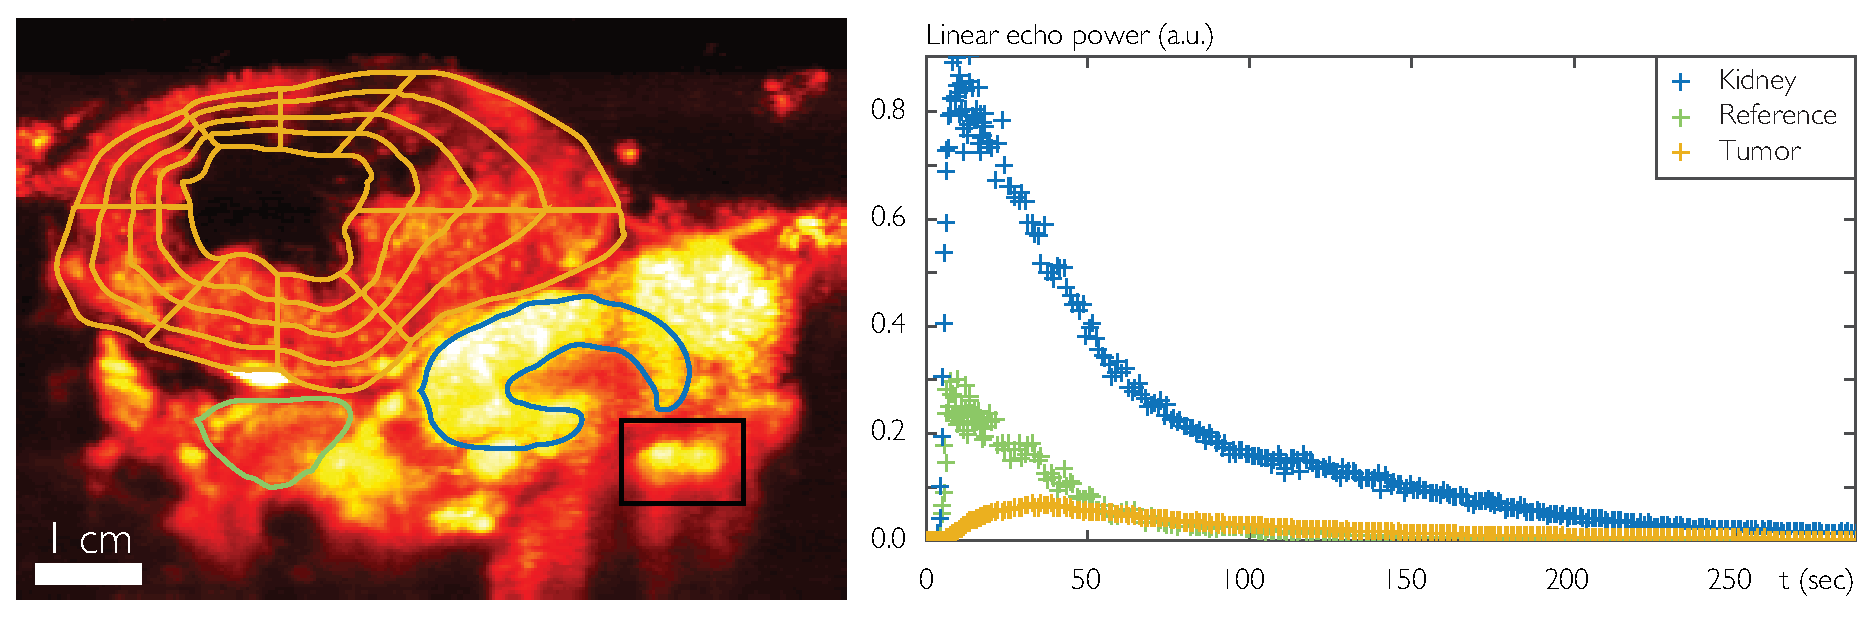
\includegraphics[width=\textwidth]{Figure1.eps}
	\caption{Illustration of the data pre-processing steps. Left: The contours of the tumor and its necrotic core have been overlaid on a  contrast enhanced image (in ochre color). The perfused tumor area was divided into 4 radial layers and 8 angular sectors. A reference tissue region (in green color) and a renal cortex region (in blue color) were also delineated. Right: Mean kinetics associated with the non-necrotic part of the tumor, the reference tissue, and the renal cortex.} 
  	\label{fig:Ch3Segmentation}
\end{figure}

\section{Methods}

\subsection{Quantification of tumor perfusion}
\label{sec:models}
Table \ref{tab:MODELS} summarizes the main features of the eight methods tested, three absolute and five relative, for tumor perfusion quantification. Some methods require the definition of an arterial region in order to estimate the AIF, its estimation is presented in section~\ref{sec:AIFmodel}. Relative quantification methods require the selection of a reference tissue region (labeled with subscript R). This region was segmented in order to define a homogeneous area, while being large enough in order to reduce noise influence on the subsequent analysis (Figure~\ref{fig:Ch3Segmentation}).

For all methods, quantitative parameters were derived by the minimization of the root-mean-square error between the time-intensity curve inside the tumor, $C_T(t)$, and the corresponding fitted curve, using an interior-point algorithm (MATLAB, MathWorks, Natick, MA, USA). To make the comparison between models easier, we focused on volume-based, flow-based, and time delays parameters.


\begin{table}
\begin{center}
\setlength{\tabcolsep}{3pt}
\begin{tabular}{llccll}
\toprule
 Acronym & Model Name & Input data & Eq. & Parameters \\
 & & AIF/RT & & & \\
\midrule
\bf{aLN} & Log-Normal & No/No &  (\ref{eq:Ch3LNmodel}) & $AUC,WIR, \Delta$ \\
\bf{aAIF} &  One-Compartment & Yes/No & (\ref{eq:CMM}) & $V,F$ \\
\bf{aAIFd} & One-Compartment with delay & Yes/No & (\ref{eq:CMM}) & $V, F, d$\\
\midrule
\bf{rLN} & Relative Log-Normal & No/Yes &  (\ref{eq:Ch3LNmodel},\ref{eq:LNr}) & $rAUC,rWIR, D$ \\
\bf{rAIF}& Relative One-Compartment & Yes/Yes & (\ref{eq:CMM},\ref{eq:AIFr})  & $ rV_{AIF},rF_{AIF}$ \\
\bf{rAIFd} &Relative One-Compartment with delay & Yes/Yes & (\ref{eq:CMM},\ref{eq:AIFr})  &  $ rV_{AIF},rF_{AIF},D_{AIF}$\\
\bf{rRT} & Relative Reference Tissue & No/Yes & (\ref{eq:RTDEF2},\ref{eq:RTparam})  & $ rV_{RT},rF_{RT}$ \\
\bf{rRTd} & Relative Reference Tissue with delay & No/Yes & (\ref{eq:RTDEF2},\ref{eq:RTparam}) & $ rV_{RT},rF_{RT},D_{RT}$ \\
\bottomrule
\end{tabular}
\caption{Synthesis of the different models tested. The first three models propose absolute quantification. The last five models propose relative quantification.}
\label{tab:MODELS}
\end{center}
\end{table}

\subsubsection{Absolute Log-normal model: aLN~\cite{Strouthos2010it}.}
The kinetics $C_T(t)$ is fitted according to the equation (\ref{eq:Ch3LNmodel}):
% \setlength{\mathindent}{30pt}
\begin{equation}
\begin{array}{rcl}
C_T(t) &= & \frac{AUC_T}{\sqrt{2 \pi}\sigma_T (t- \Delta_T)} \exp \left( - \frac{\left[ \ln{(t- \Delta_T)} - \mu_T \right]^2}{2{\sigma_T}^2} \right) \textrm{if } t > \Delta_T, \\
&=& \textrm{0 otherwise,}
\end{array}
\label{eq:Ch3LNmodel}
\end{equation}
where $AUC_T$ is the area under the $C_T$ curve, $\mu_T$  and $\sigma_T$ are the expectation and standard deviation of the distribution $C_T(\tau)/AUC_T$ when substituting $\ln(t- \Delta_T)$ with $\tau$, and $\Delta_T$ represents the time shift between the start of the acquisition and the arrival of the contrast agent in the tumor. As the area under the curve $AUC_T$ is related to the tissue blood volume~\cite{Tudorica2002at} and the wash-in rate $WIR_T$ (derived from $AUC_T$, $\mu_T$ and $\sigma_T$) is related to the tissue blood flow~\cite{Dietrich2012kw}, these two parameters were estimated in addition to $\Delta_T$ in the remaining analysis.

\subsubsection{One-Compartment model with an Arterial Input Function: \textbf{aAIF} and \textbf{aAIFd}}~\cite{Gunn2001gr}. The mathematical expression of $C_T(t)$ is given by equation (\ref{eq:CMM}):
\label{sec:AIFmodel} 
\begin{equation}
\label{eq:CMM}
\begin{array}{rcl}
C_T (t)  &= & F_T \int_{0}^{t- d_T} C_A \left( \tau \right) \exp^{-\frac{F_T}{V_T} \left( t - d_T - \tau \right)}\mathrm d \tau \quad \textrm{if } t \geq d_T,\\
&=& \textrm{0 otherwise,}
\end{array}
\end{equation}
where $C_A(t)$ is the kinetics inside the feeding artery (the AIF), $V_T$ the tissue blood volume (in \%), $F_T$ the tissue blood flow (in s$^{-1}$), and $d_T$ (in s) the time-delay of the contrast agent from the feeding artery to the tumor. When it is neglected ($d_T=0$), the model is noted \textbf{aAIF}. When it is estimated in addition to $V_T$ and $F_T$, the model is noted \textbf{aAIFd}.

To estimate the AIF, a bounding box surrounding arterial vessels was first defined according to anatomical considerations and high values of enhancement (see Figure~\ref{fig:Ch3Segmentation}).
Peak Enhancement ($PE$) and Time To Peak ($TTP$) parametric maps were then computed for each pixel of the bounding box.  The maximal value of $PE$ ($PE_{max}$) and the minimal value of $TTP$ ($TTP_{min}$) were extracted. Pixels verifying $PE/PE_{max}\geq rPE^{*}$ and $TTP-TTP_{min}\leq\Delta TTP^{*}$ were considered as part of the artery region (Figure~\ref{fig:AIF}), where $rPE^{*}$ and $\Delta TTP^{*}$ are empirically chosen cut-off values, equal to $50\%$ and 3 s, unless specified differently.
The AIF, $C_A(t)$, was computed as the geometric mean of the kinetics inside the artery region and modeled using the LN model  (\ref{eq:Ch3LNmodel}).  

\begin{figure}[ht]
  \centering
  \includegraphics[width=\linewidth]{Figure2.eps}
  \caption{Automated detection of the AIF: parametric maps $TTP$ and $PE$ inside the artery region; segmentation results and associated AIF with: (a) $rPE^{*}=50\%$ and $\Delta TTP^{*}=3$ s  (in green color); (b) $rPE^{*}=70\%$ and $\Delta TTP^{*}=2.5$ s  (in blue color).}
\label{fig:AIF}
\end{figure}

\subsubsection{Relative Log-Normal model: \textbf{rLN}.}  
This model estimates three relative parameters: the relative area under the curve $rAUC$, the relative wash-in rate $rWIR$, and the time delay between the arrival of the contrast in the tumor and the reference tissue $D_{T-R }$ according to equation~(\ref{eq:LNr}):

\begin{equation}
rAUC = \frac {AUC_T} {AUC_{R}}, \quad rWIR = \frac{WIR_T}{WIR_{R}}, \quad \textrm{and } \quad D^{T-R}_{LN} = \Delta_T - \Delta_{R},
\label{eq:LNr}
\end{equation}
where ($AUC_T$, $WIR_T$, $\Delta_T$) and  ($AUC_{R}$, $WIR_{R}$, $\Delta_{R}$) are the absolute LN parameters estimated in the tumor and in the reference tissue respectively using equation~(\ref{eq:Ch3LNmodel}).

\subsubsection{Relative One-Compartment model with an Arterial Input Function: \textbf{rAIF and rAIFd}.}
\label{sec:rAIFmodel}
This model estimates three parameters: the relative blood volume $rV_{AIF}$, the relative blood flow $rF_{AIF}$  and the  time delay between the arrival of the contrast in the tumor and the reference tissue $D^{T-R}_{AIF}$ according to equation~(\ref{eq:AIFr}):
\begin{equation}
rV_{AIF} = \frac {V_T} {V_{R}}, \quad rF_{AIF} = \frac {F_T} {F_{R}}, \quad \textrm{and } \quad D^{T-R}_{AIF} = d_T - d_{R},\\
\label{eq:AIFr}
\end{equation}
where ($V_T$, $F_T$, $d_T$) and ($V_{R}$, $F_{R}$,  $d_{R}$)  are the perfusion parameters estimated in the tumor and in the reference tissue respectively using the AIF according to equation~(\ref{eq:CMM}).
This method is referred to as \textbf{rAIF} when $D^{T-R}_{AIF} $ is set to zero and \textbf{rAIFd} otherwise. 

\subsubsection{Relative One-Compartment model using the Reference Tissue kinetics: \textbf{rRT and rRTd}}~\cite{Patlak1983id,Yankeelov2005de}.
This model estimates three parameters: the relative blood volume $rV_{RT}$, the relative blood flow $rF_{RT}$ and the time delay between the arrival of the contrast in the tumor and the reference tissue $D^{T-R}_{RT}$, the subscript $_{RT}$ being used for distinguishing this approach from the previous one (section~\ref{sec:rAIFmodel}). Assuming that the tumor and the reference region have a common AIF, the kinetics $C_{R}(t)$ and $C_{T}(t)$ can be described by equation~(\ref{eq:CMM}). When replacing $C_A(t)$ by its expression as a function of $C_R(t)$ in equation~(\ref{eq:CMM}), $C_T(t)$  can then be described by equation (5):
\begin{equation}
\begin{array}{rcl}
\hspace{-10mm}
C_T \left( t \right) & = & rF_{RT} \Big[ C_{R} \left( t - D_{RT}^{T-R} \right) \\
& & \qquad + \left( k_{R} - k_T \right) \int_{d_{R}}^{t - D_{RT}^{T-R}} C_{R} \left( \tau \right) e^{- k_T \left( t - D_{RT}^{T-R} - \tau \right)} \mathrm d \tau \Big] \quad \textrm{ if } t \geq d_T, \\
& = & \textrm{0 otherwise,}
\end{array}
\label{eq:RTDEF2}
\end{equation}
where $k_{R} = F_{R}/V_{R}$ and $k_T = F_T/V_T$. The parameter $k_{R}$ was chosen as the mean value of the $k_{R}$ values estimated with the relative AIF approach (\textbf{rAIFd}) and was set to 0.15. The parameters $rF_{RT}$, $k_T$ and$D^{T-R}_{RT}$ were estimated by solving equation~(\ref{eq:RTDEF2}). The parameter $rV_{RT}$ was then deduced using equation~(\ref{eq:RTparam}): 
\begin{equation}
rV_{RT} = \frac{V_T}{V_{R}}  = \frac{F_{T}}{k_{T}} \frac{k_{R}}{F_{R}} = rF_{RT}\frac{k_{R}}{k_T}.
\label{eq:RTparam}
\end{equation}
The method is referred to as \textbf{rRT} when $D^{T-R}_{RT}$ is set to zero and \textbf{rRTd} otherwise. 

\subsection{Data analysis}
For each model, the quantitative assessment of the fit was achieved using the normalized root mean square error ($NRMSE$), and the fraction of information that is modeled  ($FMI$), as defined in~\cite{Balvay2005ca}. The $NRMSE$ was defined by: 
\begin{equation}
NRMSE = \frac{\sqrt{\frac{1}{nt} \sum_{t=1}^{nt}\left(C_{fit}\left(t\right)-C\left(t\right)\right)^2}}{max_t(C(t))-min_t(C(t))},
\end{equation}
where $C$ and $C_{fit}$ are the observed and fitted kinetics and $nt$ is the total number of frames. 
A good fit corresponds to $NRMSE$ close to 0 and $FMI$ close to 100\%.
For each sub-region, results for which $FMI < 90\%$ were judged as poor quality fits.


In order to assess the reproducibility of the parameters $\theta^{hl}$ of the mouse $m_l$ ($l$ from 1 to 4) in the sub-region $s_h$ ($h$ from 1 to 32), coefficients of variation $CV^{hl}$  were estimated using the four test-retest studies, as follows: 
\begin{equation}
{CV^{hl}} = \frac {\sqrt {\frac{1}{4} {\sum _{k=1}^{4} (\theta^{hl}(k)- \mu^{hl})^2}}} {\mu^{hl}}, \textrm {where } \mu^{hl}=\frac{1}{4} \sum _{k=1}^{4} \theta^{hl}(k),
\label{eq:Ch3CV}
\end{equation}
$\theta^{hl}(k)$ being the parameter $\theta^{hl}$ estimated for the $kth$ test-retest study (with $k$ from 1 to 4).
As parameters $\theta^{hl}(k)$ corresponding to poor quality fits were removed, missing values were replaced using multivariate imputation according to the R package \{mice\}, 'Multivariate Imputation by Chained Equations'~\cite{vanBuuren2011ica}, in order to compute $CV^{hl}$ using four values systematically.

Statistical tests were performed to compare goodness of fit criteria and coefficients of variation between the different models, using the R package \{coin\}, 'Conditional Inference Procedures in a Permutation Test Framework'~\cite{Hothorn2008ht}. They were considered as significant when p values were less than $0.05$. As all the tests were conducted on paired data, when goodness of fit criteria were removed (due to poor quality fits), they were replaced with imputed data.
The non-parametric Friedman test with post-hoc analysis (Tukey's HSD test) was chosen for dealing with multiple comparisons. 

\section{Results}
\label{sec:results}
\subsection{Model comparison through quality of fit criteria}
\begin{table}
\begin{center}
\setlength{\tabcolsep}{4pt}
\begin{tabular}{l | rr | rrrrr}
\toprule
\multirow{2}{*}{Model} & \multicolumn{2}{c |}{All data} &  \multicolumn{3}{c}{$FMI > 90\%$}\\
& \multicolumn{2}{c |}{$NRMSE$  \quad \quad \quad \quad $FMI$} &  \multicolumn{2}{c}{$NRMSE$   \quad \quad \quad \quad $FMI$}  & $N$ \\
\midrule
\textbf{aLN}    & 5.75  [4.70-7.41]  &	99.4 [98.5-99.8] & 5.63  [4.62-7.00]	& 99.4 [98.8-99.8] &	28\\	
\textbf{aAIF} & 9.95$^{\star \dagger}$ [6.03-24.2] &  94.7$^{\star \dagger}$  [45.2-98.3] &  6.72$^\circ$ [5.12-9.20] &  97.8$^\circ$ [95.5-98.9] & 212 \\
\textbf{aAIFd} & 6.21	[4.71-8.43] & $98.7^\star$ [97.3-99.4] &  6.04  [4.66-8.20] &  $98.8^\star$ [97.6-99.4] & 19		\\
\textbf{rRT} & 7.72$^{\star \ddagger}$  [5.83-9.85] & 97.6$^{\star \ddagger}$  [94.9-98.7] &  7.45$^{\star \ddagger}$ [5.71-9.34] & 97.8$^{\star \ddagger}$ [95.6-98.8] & 56 \\
\textbf{rRTd} & 6.32 [4.91-8.21] & 98.7$^\star$ [97.2-99.4] &  6.18 [4.85-8.00]	& $98.8^\star$ [97.6-99.4]	& 19 \\
\bottomrule
\end{tabular}
\caption{Median [first-third quartiles] values of  $NMRSE$ and $FMI$ (in \%) obtained for the different models. $N$ is the  number of sub-regions where $FMI < 90\%$. Significant differences between \textbf{aLN} and any other model are indicated by $^\star$. In addition, significant differences between \textbf{aAIF} (resp. \textbf{rRT}) and \textbf{aAIFd} (resp. \textbf{rRTd)} are indicated by $^\dagger$ (resp. $^\ddagger$). The symbol $^\circ$ indicates that comparisons were not reported due to the high number of missing data.}
\label{tab:FIT}
\end{center}
\end{table}

Table~\ref{tab:FIT} shows the quartile values of the quality of fit criteria ($NRMSE$ and $FMI$), which are computed for the 512 ($4\times 4\times 32$) tumor sub-regions for the five models: \textbf{aLN}, \textbf{aAIF}, \textbf{aAIFd}, \textbf{rRT}, and \textbf{rRTd}.
Since the $NMRSE$ and $FMI$ criteria obtained by the three relative methods \textbf{rLN}, \textbf{rAIF} and \textbf{rAIFd} are identical to those obtained by \textbf{aLN}, \textbf{aAIF} and \textbf{aAIFd}, these results are not reported in Table~\ref{tab:FIT}. Additionally, quartile values are provided for the $N$ sub-regions verifying $FMI > 90\%$. 
Due to the large portion of missing data for the \textbf{aAIF} model when considering only good fits (the number of excluded regions, $N$, being equal to 212), results of hypothesis testing were not presented for that specific case. 
The \textbf{aLN} model shows slightly better quality criteria than the other models (these differences are significant for $FMI$ in all cases, and significant for $NRMSE$ in case of \textbf{aAIF} and \textbf{rRT} models). The introduction of the time delay parameter (\textbf{aAIFd},  \textbf{rAIFd} and \textbf{rRTd} models) significantly improved the modeling quality, according to both criteria. Furthermore, the number of cases for which $FMI <90\%$ was largely reduced when taking into account the time delays. For these reasons, results obtained without time delays (\textbf{aAIF}, \textbf{rAIF} and \textbf{rRT}) were not further reported.

\subsection{Model comparison through coefficients of variation}

All mean values and standard deviations of the perfusion parameters are given for each mouse in Appendix, in Table~\ref{tab:RP}.  
Figure \ref{fig:Slopes} illustrates for one specific mouse ($m_1$) the comparison between the parameters estimated by the different models. It shows a high correlation between the  volume-based parameters: $AUC$, $rAUC$, $V$, $rV_{AIF}$, and $rV_{RT}$ as well as a high correlation between the  flow-based parameters: $WIR$, $rWIR$, $F$, $rF_{AIF}$, and $rF_{RT}$. This figure shows also that there is a large range of values for each parameter within one tumor, demonstrating that perfusion parameters inside the different sub-regions of the tumor are far from being similar. Finally, it proves  that the slopes may be quite different from one study to another, and that the use of relative parameters contributes to largely reduce the differences between the test-retest studies, the estimation of $rF_{AIF}$ being less robust than the estimation of $rWIR$ or $rF_{RT}$ for this specific example. Table~\ref{tab:AIF} illustrates the influence of the AIF choice on the estimation of volume, flow, and time delay parameters. On this specific exam, two AIF were generated, the first one (AIF$_1$) with thresholds $rPE^{*}=50\%$ and $\Delta TTP^{*}=3$ s, the second one (AIF$_2$) with thresholds $rPE^{*}=70\%$ and $\Delta TTP^{*}=2.5$ s (as shown in Figure~\ref{fig:AIF}). The variations were very large for $V$ and $F$ parameters, while they remained moderate for $rF_{AIF}$ and time delays, and very low for $rV_{AIF}$.

\begin{figure}[ht]
  \centering
  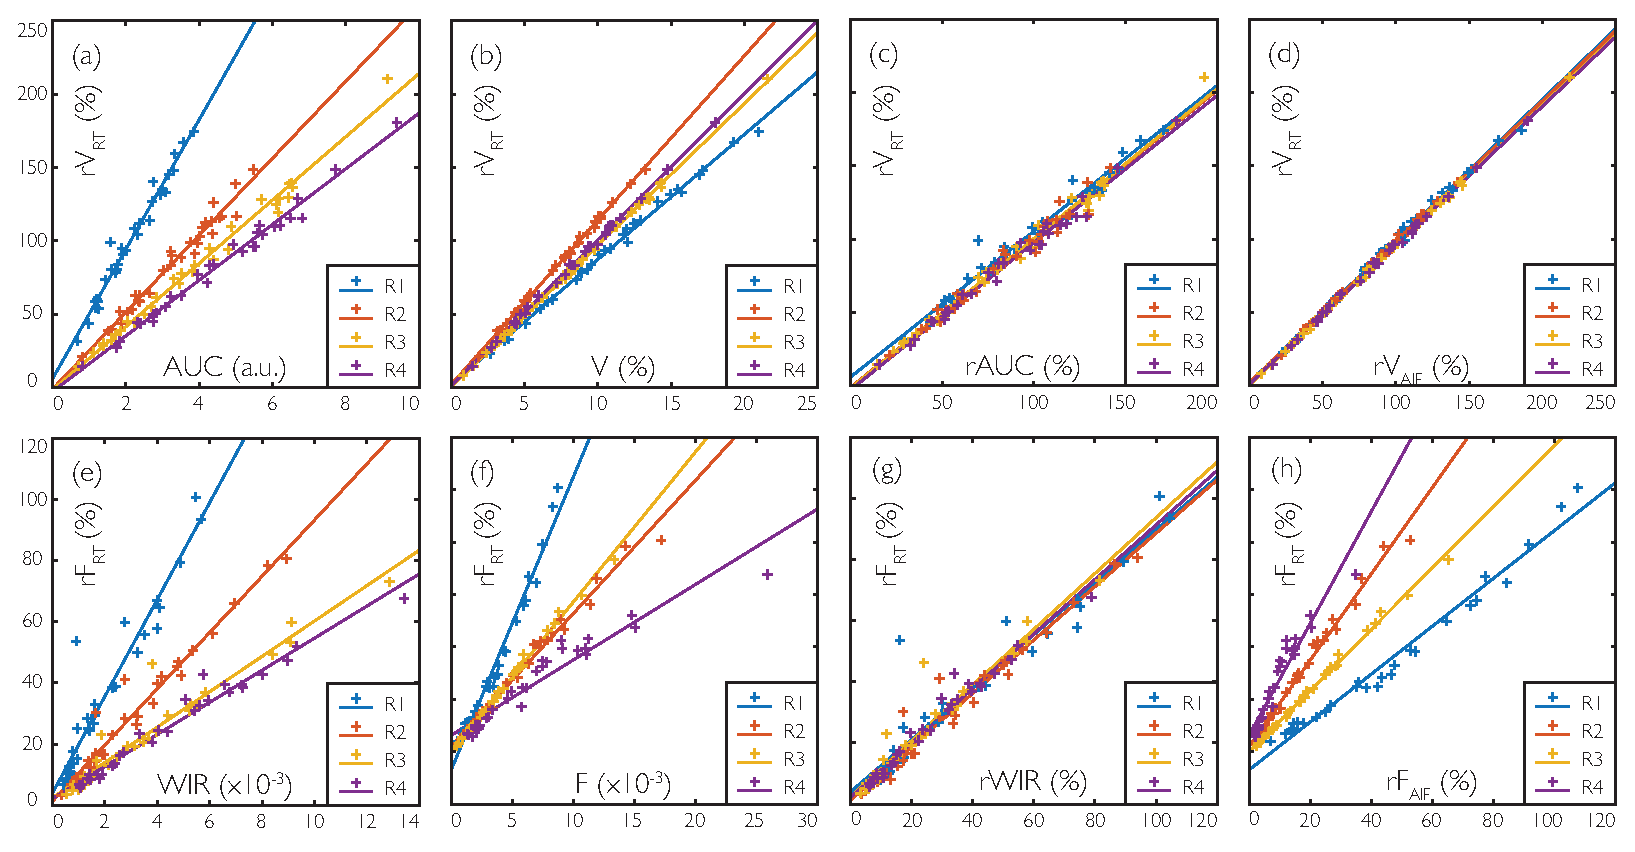
\includegraphics[width=\linewidth]{Figure3.eps}
  \caption{Comparison of the volume-based and flow-based parameters obtained for the four test-retest exams ($R_1$, $R_2$, $R_3$, and $R_4$) of the mouse $m_1$: linear regressions between (a) $rV_{RT}$ and $AUC$, (b) $rV_{RT}$ and $V$, (c) $rV_{RT}$ and $rAUC$, (d) $rV_{RT}$ and $rV_{AIF}$, (e) $rF_{RT}$ and $WIR$, (f) $rF_{RT}$ and $F$, (g) $rF_{RT}$ and $rWIR$, (h) $rF_{RT}$ and $rF_{AIF}$.}
\label{fig:Slopes}
\end{figure}

\begin{table}[ht]
\begin{center}
\begin{tabular}{ccccccc}
\toprule
& $V$ (\%) & $rV_{AIF} (\%) $ & $F$ ($10^{-3}$ s$^{-1}$) & $rF_{AIF}$ (\%)& $d_T$ (s) & $D_{AIF}^{T-R}$ (s) \\
\midrule
AIF$_1$ & $8.02 \pm 3.89$ 	& $84.5 \pm 40.9$ 
		& $6.54 \pm 5.37$ 	& $8.83 \pm 7.24$ 
		& $2.4 \pm 3.4$ 	& $1.4 \pm 3.4$ \\
AIF$_2$ &$4.65 \pm 2.25$ 	& $85.2 \pm 41.3$ 
		& $3.20 \pm 2.61$ 	& $10.1 \pm 8.21$ 
		& $2.0 \pm 3.3$ 	& $1.6 \pm 3.3$ \\
\bottomrule
\end{tabular}
\caption{Mean $\pm$ standard deviation of the parameters estimated with the \textbf{aAIFd} and  \textbf{rAIFd} models, using two different sets of cut-offs to generate the AIF functions.}
\label{tab:AIF}
\end{center}
\end{table}

\begin{figure}[ht]
  \centering
  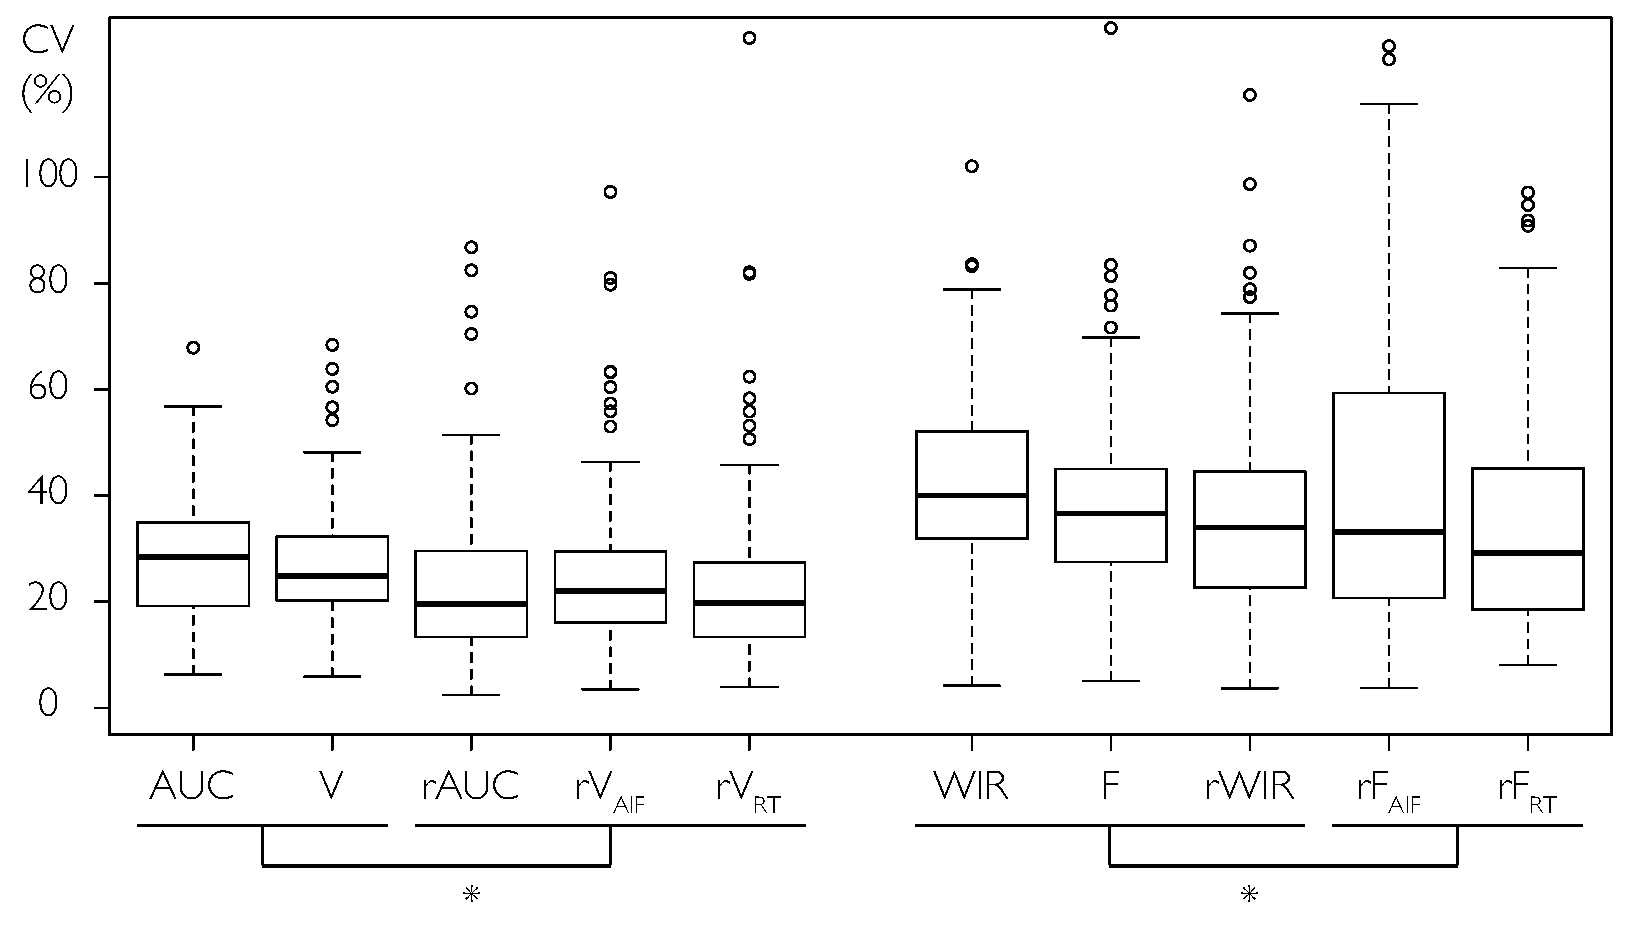
\includegraphics[width=\linewidth]{Figure4.eps}
  \caption{Boxplot showing the coefficients of variation of blood volume parameters (left) and blood flow parameters (right) estimated with the \textbf{aLN}, \textbf{rLN}, \textbf{aAIFd}, \textbf{rAIFd}, and \textbf{rRTd} models. For each box, the bold line represents the median value, the bottom and top lines the first and third quartiles. Dotted lines extend to the most extreme data points which are less than 1.5 times the interquartile range. Outlier points are displayed with empty circles. Two groups of parameters were built (horizontal lines below the parameter names) such that there were no significant intra-group differences while there were statistically significant inter-group differences (marked by $^{*}$).}
\label{fig:CV}
\end{figure}

Finally, Figure~\ref{fig:CV} shows the distributions of the coefficients of variation of volume-based and flow-based parameters, computed according to equation (\ref{eq:Ch3CV}). Relative volume parameters ($rAUC$, $rV_{AIF}$, and $rV_{RT}$) have significantly lower CV than absolute volume parameters ($AUC$ and $V$). No significant difference was found when comparing $WIR$, $F$, and $rWIR$, but the CV of these parameters are significantly higher than those of $rF_{AIF}$ and $rF_{RT}$.
Numerical values of these mean CV are given for each mouse in Appendix, in Table~\ref{tab:RCV}.


\section{Discussion}
Using a test-retest study with a controlled bolus injection, it was possible to assess the variability of DCE-US perfusion parameters. To reduce this variability, the interest of estimating relative parameters, which necessitates the definition of a reference tissue region, was practically demonstrated. Our study also shows the importance of choosing an appropriate method for the estimation of the parameters, because estimation methods have an impact on parameter variability. Thus the reference tissue approach (\textbf{rRTd}) can be recommended, since it is the most robust method when considering the volume-based and the flow-based parameters simultaneously.

The recommendations of the EFSUMB for DCE-US quantification in oncology suggest to estimate  parameters such as $AUC$ and $WIR$ from explicitly defined models, e.g.~using the \textbf{aLN} model. To reduce the variability of the estimated parameters, Dizeux et al. proposed a controlled injection system~\cite{Dizeux2016cd}. However, the present study shows that the differences between two consecutive exams are still not negligible for a regional analysis. Since in PET and DCE-MRI, deconvolution approaches and compartmental models have proved their efficiency to make parameters more robust to inter-exam changes, we decided to test some of these approaches. The most commonly used methods require the estimation of an arterial input function. Deconvolution approaches were recently proposed to quantify tissue perfusion in DCE-US~\cite{Gauthier2012vc}. These approaches estimate the transfer function of the system (depending on a large number of parameters), and to avoid aberrant solutions, this estimation needs to be regularized. 
Following this idea, the one-compartment model with time delay is a deconvolution depending on three parameters only. When the time delay is set to 0,  (\textbf{aAIF} model), we have shown that the quality of fit is worse than the one obtained when using the explicit \textbf{aLN} model. 
When introducing a time delay parameter, an option that is unfortunately generally overlooked~\cite{Kudo2009hy}, a much more accurate fit of regional tumor kinetics was obtained. Indeed, the quality of fit using \textbf{aLN} (depending on four parameters) and this  \textbf{aAIFd} model was equivalent in terms of $NRMSE$. 

Our study shows the crucial role of the AIF estimation in the variability of the perfusion parameters (see Table~\ref{tab:AIF}). When focusing the field of view in the main plane of the tumor, it can be difficult to estimate the AIF robustly (see Figure~\ref{fig:AIF}). Indeed, AIF measurements in small vessels can be affected by partial volume effects, yielding underestimation of the signal intensity. Thus coefficients of variation deduced from the \textbf{aAIFd} model can be high. Note that some problems could also occur in larger vessels, including non-linearities between concentration and measured signal, and attenuation artifacts ~\cite{Mule2008ms}.

The use of relative parameters was suggested to overcome the difficulties of estimating the AIF for a compartmental model in DCE-MRI ~\cite{Yankeelov2005de}. Clinical studies have reported the interest of estimating normalized perfusion parameters in DCE-US \cite{Guibal2010bl,Hoeffel2010ce,Lefort2012km}. Using systematically three models (\textbf{rLN}, \textbf{rAIFd}, \textbf{rRTd}), our study reinforces the interest of estimating relative parameters. The choice of a reference tissue region is less critical than the segmentation of an artery. Indeed, a larger structure can be used, reducing segmentation errors and the impact of partial volume effect. Furthermore, as the contrast concentration is lower, the quantification errors due to non-linearity are reduced. Kidney regions were initially tested but finally excluded because of the overlap of cortical, proximal tubular and distal tubular compartments. Muscular regions that could be delineated on the four exams were finally chosen.

Recirculation is a major problem when dealing with modeling techniques adapted to first-pass studies. However, its quantitative impact is reduced in DCE-US when compared to other modalities since the destruction of microbubbles, in the lungs in particular, makes the number of microbubbles much smaller in the second pass (and following) than it is in the first pass. We deliberately did not try to model the recirculation, when we chose the \textbf{aLN} model to fit tumor kinetics or when we first fit the AIF using the \textbf{aLN} model. In addition, using simulated data, we showed that the practical impact on parameters estimation when neglecting the recirculation was limited, especially for relative parameters, since the coefficients of variation between parameters estimated with and without simulating the recirculation effect were less than the ones estimated through the test-retest studies (this recirculation effect was about 5\% on CV values with the \textbf{rRTd} approach).

The use of normalized parameters induced a significant reduction of coefficients of variation in our test-retest study. 
Furthermore, estimating relative volume and flow parameters using equation~(\ref{eq:RTDEF2}), which eliminates the need for an AIF, is more robust than using the AIF directly. It should also be noted that the small 3D displacements occurring between the four test-retest studies can partly explain the CV, due to the imperfect spatial alignment between sub-regions from one exam to the following one.

 Figure~\ref{fig:Slopes} reveals strong correlations between the different parameters computed inside a same sub-region, and a large variation of these parameters according to the tumor sub-regions. Thus, whatever the model used,  all the flow-based or volume-based parameters can reveal spatial tumor heterogeneity. However, when it comes to the comparison of longitudinal exams, it is crucial to have comparable parameter values. Thus, the estimation of relative parameters seem to be the most powerful solution, provided that the reference tissue characteristics are not modified between exams.
Some interesting results have been recently shown~\cite{Wang2015bb} for a longitudinal study using a 3D DCE-US approach. Compared with the 2D approach, the 3D approach enables assessment of the whole tumor and should be preferred for tumor monitoring.

 \section{Conclusion}
This study aimed at proposing valuable modeling of DCE-US studies to estimate reliable perfusion parameters in a murine model of tumor. First, it was shown that a one-compartment model based on an AIF, and completed by the estimation of a time-delay parameter, could fit kinetics as closely as the explicit log-normal model. Second, a comprehensive comparison of the parameters estimated by different approaches was proposed, showing high correlations between the volume-based  and flow-based parameters respectively estimated. Based on test-retest studies with controlled injections, a large variability (up to 40\%) of regional perfusion parameters was established due to the inherent variations of experimental and physiological conditions for the log-normal modeling and to the difficulties in estimating a correct AIF in the image field of view for the compartmental approach. To reduce this variability, the use of relative values of these regional perfusion parameters was proposed, requiring in all cases the delineation of a reference tissue region. To estimate these relative parameters, the reference tissue model proved to be the most reliable computing approach. Thus we recommend the use of this model to estimate reliable relative perfusion parameters.

\section{Acknowledgments}
The authors are grateful to the anonymous reviewers for their valuable comments on the paper.
This work was funded by the Fondation pour la Recherche M\'edicale through the Bioing\'enierie pour la Sant\'e research grant DBS20131128436. Research was also supported by the Institut Universitaire d{'}Ing\'enierie en Sant\'e, Sorbonne Universit\'e, Projet OCSCC 2014/2016.
Experiments were performed on a platform of France Life Imaging partly funded by the grant ANR-11-INBS-0006 associated within the Plateforme Imagerie du Vivant. All the animals were house kept at Centre d{'}Ex-plorations Fonctionnelles of Centre de Recherche des Cordeliers, Agreement A75-06-12.


\section*{References}
\bibliographystyle{plainnat}
\bibliography{Bibliography/chap3}

\section* {Appendix}
This appendix gives the numerical results that were obtained for each mouse ($m_1$, $m_2$, $m_3$, and $m_4$), including mean values and standard deviations of regional parameters (Table \ref{tab:RP}) and coefficients of variation of these parameters (Table \ref{tab:RCV}). 

\begin{table} [hb]
\begin{center}
\begin{tabular}{lccccc}
\toprule
& \multicolumn{2}{c}{Absolute parameters} & \multicolumn{3}{c}{Relative parameters} \\
\midrule
 & $AUC$ (a.u.) & $V$ (\%)  & $rAUC$ (\%) & $rV_{AIF}$ (\%)  & $rV_{RT}$ (\%)  \\
\midrule
$m_1$  	& $3.47 \pm 1.82$ 	& $8.61 \pm 4.31$ 	& $87.2 \pm 37.9$ 	& $87.6 \pm 41.5$ 	& $85.9 \pm 41.2$ 	\\
$m_2$  	& $5.97 \pm 2.08$ 	& $17.6 \pm 6.60$ 	& $11.2 \pm 3.19$ 	& $18.1 \pm 6.25$ 	& $13.2 \pm 3.51$ 	\\
$m_3$  	& $6.74 \pm 3.51$ 	& $12.9 \pm 6.40$ 	& $144 \pm 81.3$ 	& $131 \pm 73.0$ 	& $132 \pm 75.2$ 	\\
$m_4$  	& $7.90 \pm 4.23$ 	& $21.2 \pm 11.6$ 	& $57.9 \pm 30.6$ 	& $62.3 \pm 33.1$ 	& $59.4 \pm 31.6$ 	\\
\midrule
& $WIR$ (a.u. s$^{-1}$)  & $F$ (s$^{-1}$) & $rWIR$ (\%) & $rF_{AIF} (\%) $ & $rF_{RT}$ (\%) \\
\midrule
$m_1$ 	& $3.30 \pm 2.66$ 	& $4.94 \pm 4.07$ 	& $29.7 \pm 23.4$ 	& $21.9 \pm 21.9$ 	& $27.0 \pm 20.3$ 	\\
$m_2$ 	& $4.70 \pm 3.03$ 	& $6.49 \pm 3.45$ 	& $17.7 \pm 10.2$ 	& $17.2 \pm 8.34$ 	& $16.1 \pm 11.0$ 	\\
$m_3$  	& $4.88 \pm 4.19$ 	& $3.64 \pm 2.90$ 	& $32.9 \pm 28.6$ 	& $36.4 \pm 27.7$ 	& $25.1 \pm 21.0$ 	\\
$m_4$  	& $6.63 \pm 5.30$ 	& $5.21 \pm 3.59$ 	& $23.7 \pm 19.0$ 	& $26.4 \pm 18.2$ 	& $18.0 \pm 13.6$ 	\\
\midrule
Delay & $\Delta$ (s) & $d$ (s)& $D^{T-R}_{LN}$ (s)& $D_{AIF}^{T-R}$ (s)  & $D_{RT}^{T-R}$ (s) \\
\midrule
$m_1$  	& $5.5 \pm 3.4$		& $3.2 \pm 4.1$		& $-1.9 \pm 3.4$	& $2.7 \pm 4.2$ 	& $3.9 \pm 4.7$	\\
$m_2$  	& $2.8 \pm 2.5$		& $5.7 \pm 4.7$		& $0.7 \pm 2.4$		& $4.2 \pm 4.5$ 	& $5.3 \pm 4.0$ \\
$m_3$ 	& $3.2 \pm 2.8$		& $7.4 \pm 5.6$		& $0.4 \pm 3.1$		& $3.6 \pm 5.5$ 	& $4.4 \pm 5.8$ \\
$m_4$  	& $4.4 \pm 2.4$		& $7.0 \pm 4.6$		& $-0.8 \pm 2.3$	& $5.9 \pm 4.5$ 	& $5.6 \pm 4.7$ \\
\bottomrule
\end{tabular}
\caption{Mean $\pm$ standard deviation of the volume, flow and delay parameters estimated in the different sub-regions of the tumor, for the four test-retest exams, after multiple imputation of missing values due to poor fit quality. Values of $WIR$ and $F$ are multiplied by 1000.}
\label{tab:RP}
\end{center}
\end{table}

\begin{table}
\begin{center}
\begin{tabular}{lccccc}
\toprule
& \multicolumn{2}{c}{Absolute parameters} & \multicolumn{3}{c}{Relative parameters} \\
\midrule
 & $CV_{AUC}$  & $CV_{V}$  & $CV_{rAUC}$  & $CV_{rV_{AIF}}$  & $CV_{rV_{RT}}$ \\
\midrule
$m_1$  	& $34.7 \pm 10.6$ 	& $30.2 \pm 17.1$ 	& $22.4 \pm 14.4$ 	& $24.6 \pm 17.5$ 	& $24.7 \pm 17.3$ 	\\
$m_2$  	& $26.2 \pm 6.83$ 	& $26.7 \pm 9.85$ 	& $15.0 \pm 6.51$ 	& $21.8 \pm 9.99$ 	& $15.3 \pm 7.01$ 	\\
$m_3$ 	& $31.0 \pm 12.3$ 	& $26.6 \pm 10.9$ 	& $37.2 \pm 16.8$ 	& $35.2 \pm 17.8$ 	& $35.2 \pm 18.7$ 	\\
$m_4$ 	& $20.7 \pm 10.6$ 	& $23.3 \pm 9.93$ 	& $18.8 \pm 8.68$ 	& $19.0 \pm 7.61$ 	& $17.8 \pm 8.17$ 	\\

\midrule
 & $CV_{WIR}$  & $CV_{F}$  & $CV_{rWIR}$ & $CV_{rF_{AIF}}$ & $CV_{rF_{RT}}$ \\
\midrule
$m_1$ 	& $42.4 \pm 12.4$ 	& $35.4 \pm 12.5$ 	& $33.4 \pm 14.9$ 	& $75.5 \pm 19.9$ 	& $29.6 \pm 13.2$ 	\\
$m_2$ 	& $44.4 \pm 11.0$ 	& $34.4 \pm 7.23$ 	& $27.4 \pm 10.9$ 	& $23.4 \pm 9.94$ 	& $33.1 \pm 18.7$	\\
$m_3$ 	& $45.3 \pm 18.5$ 	& $46.9 \pm 17.7$ 	& $50.9 \pm 17.7$ 	& $36.8 \pm 16.6$ 	& $38.3 \pm 21.3$ 	\\
$m_4$  	& $34.9 \pm 18.9$ 	& $33.3 \pm 17.3$ 	& $38.3 \pm 21.2$ 	& $27.1 \pm 13.7$ 	& $29.4 \pm 15.8$ 	\\

\bottomrule
\end{tabular}
\caption{Mean $\pm$ standard deviation of the coefficients of variation (CV), expressed in percentage, of volume and flow parameters estimated for each sub-region after multiple imputation of missing values due to poor fit quality. CV were not computed for time delays, since their values can be either positive or negative.}
\label{tab:RCV}
\end{center}
\end{table}
\part{Proposition and assessement of a new quantification method}
\chapter{Relations between perfusion parameters: theoretical and experimental considerations}\label{chapter:PMB2}
\section{Introduction}
This chapter is a complement to the work presented in Chapter~\ref{chapter:PMB}, and relies on the same experimental data, mathematical models, and notations.
It aims at establishing the relations between the semi-quantitative perfusion parameters commonly derived from the Log-Normal model, and the relations between these parameters and the quantitative parameters of the one-compartment model.
The relations between parameters were first established theoretically, and then experimentally through correlation studies.

\section{Theory}
This section gives the closed-form expressions of $AUC$, $PE$, $TTP$, $MTT$, $WIR$, $WOR$, and $TD$ parameters for the Log-Normal model, \textbf{aLN} (Table \ref{tab:AnalyticRelation}), and for the one-compartment model, \textbf{aAIFd} (Table \ref{tab:AnalyticRelationAIF}).
The equations of the models are given in Section~\ref{sec:models} of Chapter~\ref{chapter:PMB}.

$AUC$ was defined as the infinite integral of the function, $PE$ as the value taken by the function where its derivative is null, $TTP$ the time where the function derivative is null, $MTT$ as the expected value of the function normalized by its $AUC$, the $WIR$ and $WOR$ as the derivative of the function where its second order derivative is null, and $TD$ as the time-delay of the function.

\begin{table}[!h]
\begin{center}
\begin{tabular}{lc}
\toprule
\textbf{$AUC$} & $A$ \\
\midrule
\textbf{$TTP$} & $e^{\mu - \sigma^2}$  \\
\midrule
\textbf{$PE$} & $A\frac{e^{\frac{\sigma^2}{2}-\mu}}{\sigma \sqrt{2\pi}}$  \\
\midrule
\textbf{$MTT$} & $e^{\mu + \frac{\sigma^2}{2}}$ \\
\midrule
\textbf{$WIR$}
 & $\frac{A}{\sigma\sqrt{2\pi}}\left(\frac{y}{\sigma^2}-1\right)e^{2y-2\mu-\frac{y^2}{2\sigma^2}}$, where $y = \frac{3\sigma^2+\sigma\sqrt{\sigma^2+4}}{2}$ \\
\midrule
\textbf{$WOR$} & $\frac{A}{\sigma\sqrt{2\pi}}\left(1-\frac{z}{\sigma^2}\right)e^{2z-2\mu-\frac{z^2}{2\sigma^2}}$, where $z = \frac{3\sigma^2-\sigma\sqrt{\sigma^2+4}}{2}$ \\
\midrule
\textbf{$TD$} & $\Delta_T$ \\
\bottomrule
\end{tabular}
\caption{Closed-form expressions of perfusion parameters using the \textbf{aLN} model, WOR being the absolute value of the maximum negative slope.}
\label{tab:AnalyticRelation}
\end{center}
\end{table}

\begin{table}[!h]
\begin{center}
\begin{tabular}{lccc}
\toprule
AIF & \textbf{$K\delta\left(t\right)$} & $K rect_a\left(t\right)$ & $C_A \left(t\right)$ \\
\midrule
\textbf{$AUC$} & $KV_T$ & $KV_T$ & $V_T \int_{0}^{+\infty}C_A\left(\tau\right)\mathrm d\tau$\\
\midrule
\textbf{$TTP$} & 0  & $a$ & $\{ t_P \enskip\vert\enskip C_T\left(t_P - d_T\right) = V_T C_A\left(t_P \right)\}$ \\
\midrule
\textbf{$PE$} &  $KF_T$ & $\frac{KV_T}{a}\left(1-e^{-\frac{aF_T}{V_T}}\right)$ & $F_Te^{-\frac{F_T}{V_T} t_P}\int_{0}^{t_P}C_A\left(\tau\right)e^{\frac{F_T}{V_T} \tau}\mathrm d\tau$ \\
\midrule
\textbf{$MTT$} & $\frac{V_T}{F_T}$ & $\frac{V_T}{F_T} + \frac{a}{2}$ & $\frac{V_T}{F_T} + MTT_{C_A}$ \\
\midrule
\multirow{2}{*}{\textbf{$WIR$}}
 &  \multirow{2}{*}{$\infty$} & \multirow{2}{*}{{$\frac{KF_T}{a}$}} & $F_T\left(C_A\left(t_{I}\right)-\frac{1}{V_T}C_T\left(t_{I} - d_T\right)\right)$ \\
&  & & $\{ t_{I} \enskip\vert\enskip \frac{\mathrm d C_T}{\mathrm dt}\left(t_{I} - d_T\right) = V_T \frac{\mathrm d C_A}{\mathrm dt}\left(t_{I}\right), \frac{\mathrm d C_A}{\mathrm d t}\left(t_{I}\right) > 0\}$ \\
\midrule
\multirow{2}{*}{$WOR$} &  \multirow{2}{*}{$\frac{KF_T^2}{V_T}$} & \multirow{2}{*}{$\frac{KF_T}{a}\left( 1-e^{-\frac{aF_T}{V_T}} \right)$} & $F_T\left(C_A\left(t_{O}\right)-\frac{1}{V_T}C_T\left(t_{O} - d_T\right)\right)$ \\
& & & $\{ t_{O} \enskip\vert\enskip \frac{\mathrm d C_T}{\mathrm d t}\left(t_{O} - d_T\right) = V_T \frac{\mathrm d C_A}{\mathrm d t}\left(t_{O}\right),\frac{\mathrm d C_A}{\mathrm d t}\left(t_{O}\right) < 0\}$ \\
\midrule
$TD$ & $d_T$ & $d_T$ & $d_T$ \\
\bottomrule
\end{tabular}
\caption{Closed-form expressions of perfusion parameters using a one-compartment model (\textbf{aAIFd}) and assuming three different shapes of AIF: impulse function $(\delta)$, rectangle function of width $a$ and height $1/a$, $rect_a(t)$, and general case $C_A(t)$. In the first two cases, $K$ stands for the injected concentration. In the general case, $MTT_{C_A}$ stands for the mean transit time of $C_A(t)$.}
\label{tab:AnalyticRelationAIF}
\end{center}
\end{table}

\begin{table}[!h]
\begin{center}
\begin{tabular}{lccc}
\toprule
AIF & \textbf{$K\delta\left(t\right)$} & $K rect_a\left(t\right)$ & $C_A \left(t\right)$ \\
\midrule
\textbf{$rAUC$} & $\frac{V_T}{V_R}$ & $\frac{V_T}{V_R}$ & $\frac{V_T}{V_R}$\\
\midrule
\multirow{3}{*}{\textbf{$rWIR$}} &  \multirow{3}{*}{--} & \multirow{3}{*}{{$\frac{F_T}{F_R}$}} & $\frac{F_T\left(C_A\left(t_{I,T}\right)-\frac{1}{V_T}C_T\left(t_{I,T} - d_T\right)\right)}{F_R\left(C_A\left(t_{I,R}\right)-\frac{1}{V_R}C_R\left(t_{I,R} - d_R\right)\right)}$ \\
&  & & $\{ t_{I,T} \enskip\vert\enskip \frac{\mathrm d C_T}{\mathrm dt}\left(t_{I,T} - d_T\right) = V_T \frac{\mathrm d C_A}{\mathrm dt}\left(t_{I,T}\right), \frac{\mathrm d C_A}{\mathrm d t}\left(t_{I,T}\right) > 0\}$ \\
&  & & $\{ t_{I,R} \enskip\vert\enskip \frac{\mathrm d C_R}{\mathrm dt}\left(t_{I,R} - d_R\right) = V_R \frac{\mathrm d C_A}{\mathrm dt}\left(t_{I,R}\right), \frac{\mathrm d C_A}{\mathrm d t}\left(t_{I,R}\right) > 0\}$ \\
\midrule
$rTD$ & $d_T - d_R$ & $d_T - d_R$ & $d_T - d_R$ \\
\bottomrule
\end{tabular}
\caption{Closed-form expressions of the relative perfusion parameters using a relative one-compartment model (\textbf{rAIFd}) and assuming three different shapes of AIF: impulse  function $(\delta)$, rectangle function of width $a$ and height $1/a$, $rect_a(t)$, and general case $C_A(t)$. In the first two cases, $K$ stands for the injected concentration.}
\label{tab:AnalyticRelationRelative}
\end{center}
\end{table}

\section{Data Analysis}
Coefficients of determination $R^2_{\theta_{i},\theta_{j}}$ were estimated from the least-squares linear regression between the 32 regional estimates of parameters $\theta_{i}^{h}$ and $\theta_{j}^{h}$, one estimate per sub-region $s_{h})$. These coefficients were computed independently for each of the 16 DCE-US studies (4 mice $m_{l}$ $\times$ 4 test-restest studies $R_{k}$). A linear regression was also computed between sets of $512$ parameters (the 32 sub-regions of the 16 studies were polled together) to assess the consistency of the relationships between parameters. 

\section{Results}
\begin{figure}[ht]
  \centering
  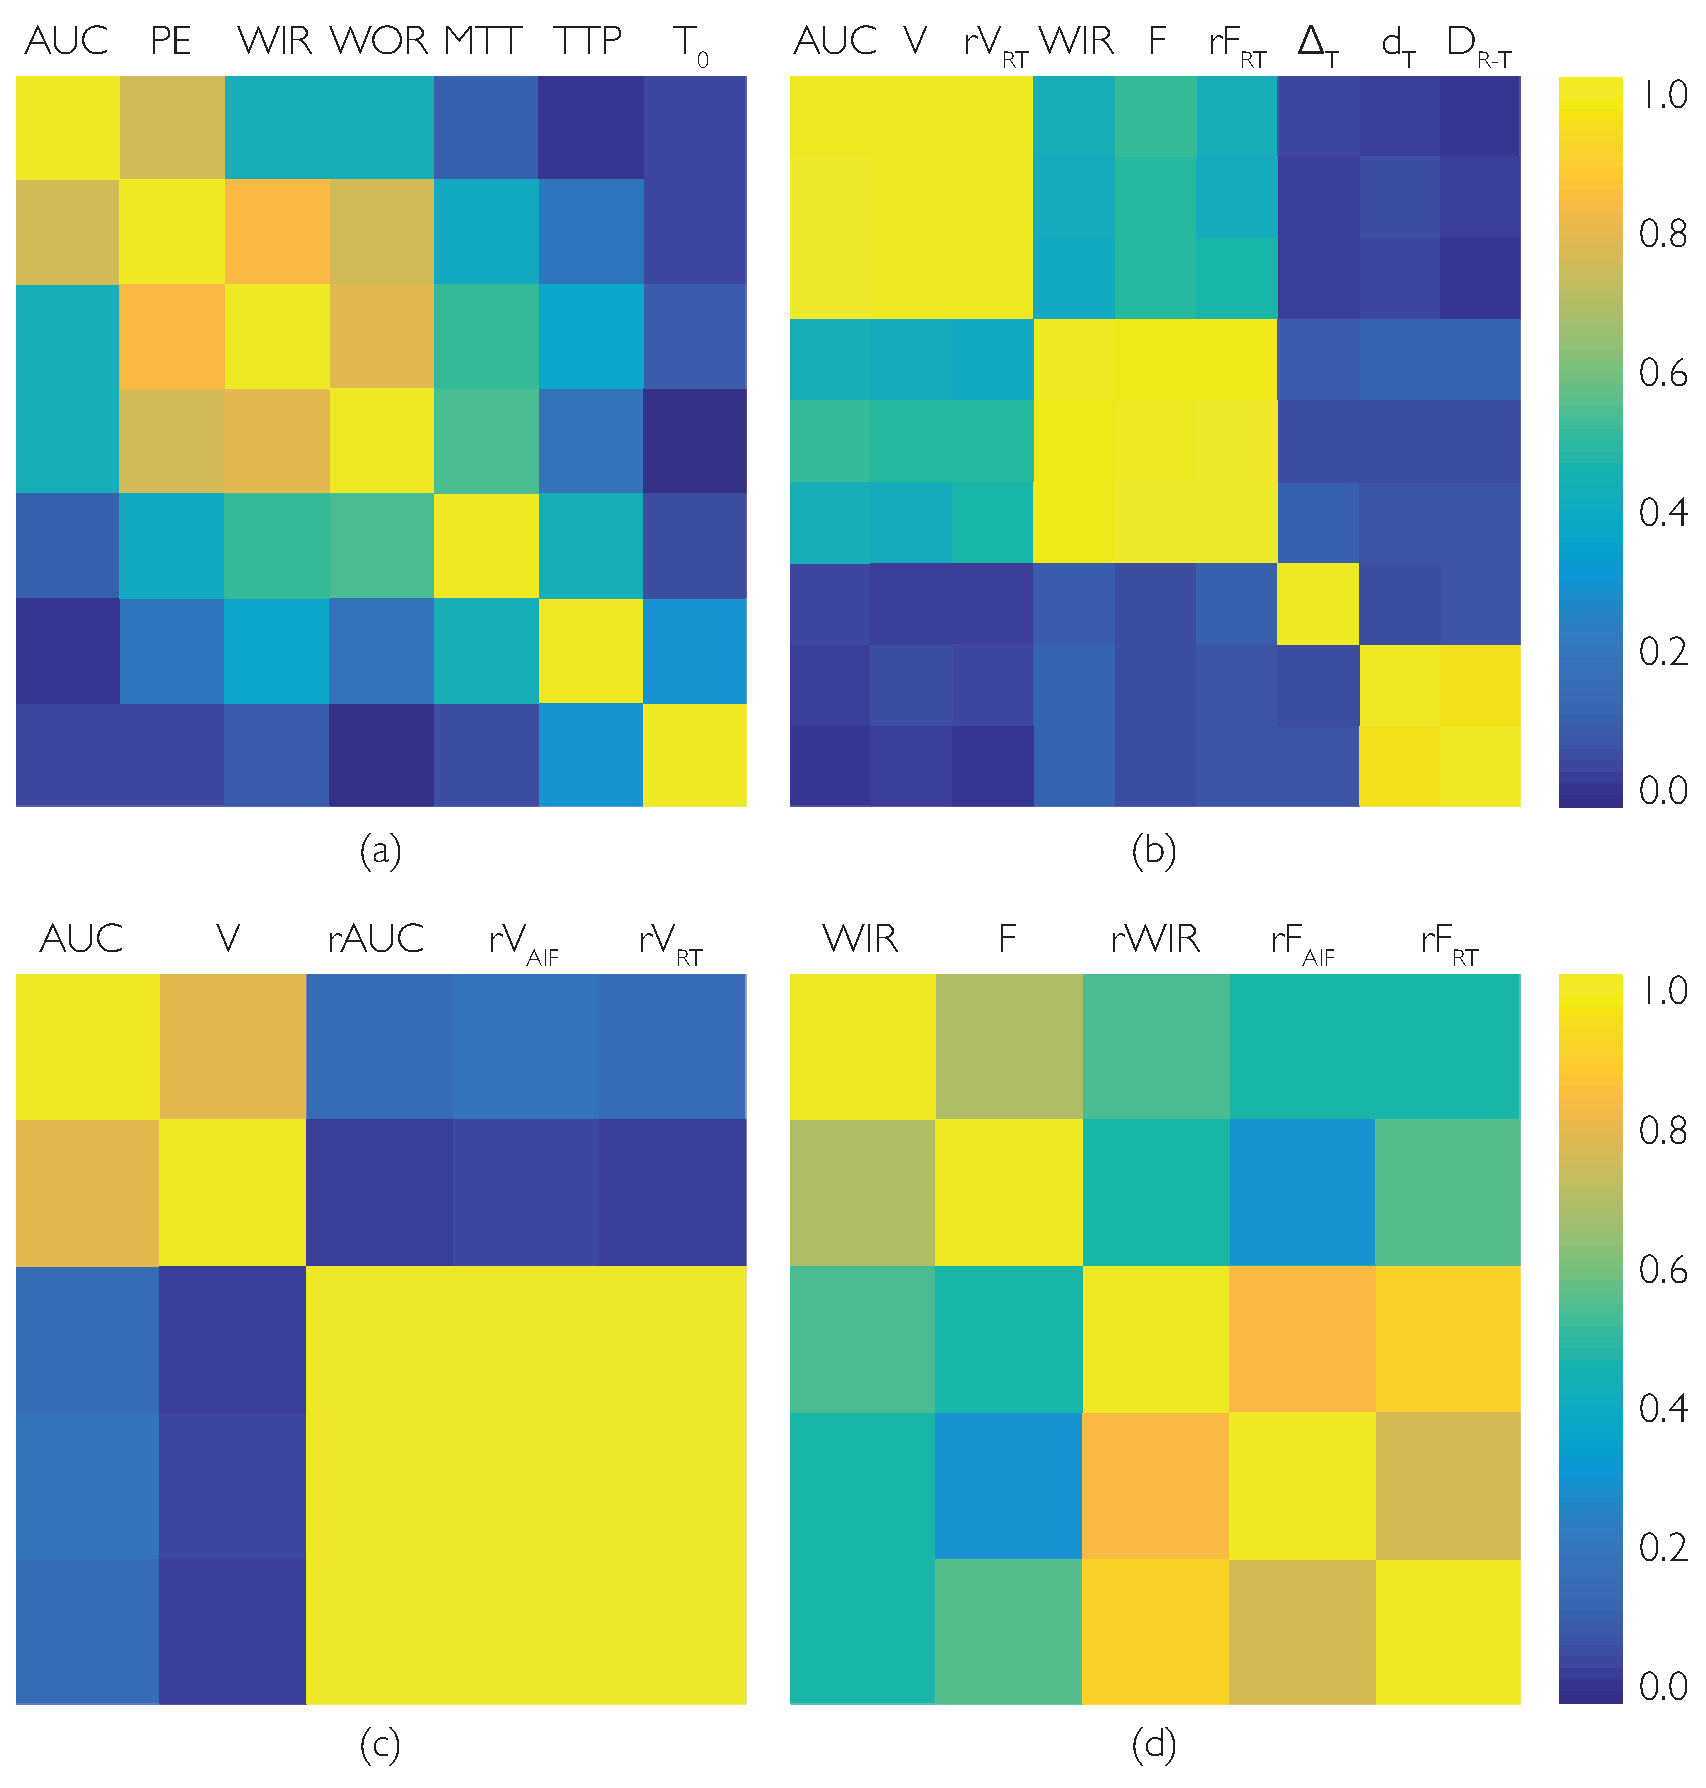
\includegraphics[width=\linewidth]{R2HeatMap.eps}
  \caption{(a-b) Median (of $16$ values) coefficient of determination ($R^2$) of the least-squares linear regression between pairs of parameters $\left(\theta_i, \theta_j\right)$ computed for the 32 sub-regions of one exam: (a)~parameters derived from the \textbf{aLN} approach; (b)~volume ($AUC$, $V$ and $rV_{RT}$ ), flow ($WIR$, $F$ and $rF_{RT}$) and time delay ($\Delta_T$ , $d_t$ and $D_{RT}$) parameters respectively computed with \textbf{aLN}, \textbf{aAIFd}  and \textbf{RTd} models. (c-d) Coefficients of determination ($R^2$) of the least-squares linear regression computed when pooling the 512 sub-regions  together: (c) $R^2$ between pairs of volume parameters computed with \textbf{aLN}, \textbf{aAIFd}, \textbf{rLN}, \textbf{rAIFd}  and \textbf{RTd} models, (d) $R^2$ between pairs of flow parameters computed with \textbf{aLN}, \textbf{aAIFd}, \textbf{rLN}, \textbf{rAIFd} and \textbf{RTd} models.}
  \label{fig:R2HeatMaps}
\end{figure}

The heatmaps shown in Figure~\ref{fig:R2HeatMaps} correspond to $R^2_{\theta_{i}\theta_{j}}$ coefficients from the linear regressions between pairs of parameters $\left(\theta_{i}, \theta_{j}\right)$. Figure~\ref{fig:R2HeatMaps}~(a) shows the $R^2$ coefficients between all pairs of parameters derived from the \textbf{aLN} model. It reveals strong linear relationships between some of the parameters, especially $\mathrm{median}\left(R^2_{AUC, PE}\right)$, $\mathrm{median}\left(R^2_{PE, WIR}\right)$, $\mathrm{median}\left(R^2_{WIR, WOR}\right)$. The formal non-linear relationships between these parameters (expressed in Table~\ref{tab:AnalyticRelation}) generate high linear links and thus information redundancy. For that reason we further focused on three derived parameters: $AUC$, which is related to tissue blood volume $V$, according to the closed-form expressions given in Table~\ref{tab:AnalyticRelationAIF}, $WIR$, which is mainly related to tissue blood flow $F$), and the delay parameter $\Delta$. In addition, Table~\ref{tab:AnalyticRelationRelative} shows the formal relations between the relative value of $AUC$ ($rAUC$) and $WIR$ ($rWIR$) and the parameters of the \textbf{aAIFd} model. It reveals that $rAUC$ and $rV$ are equivalent, and that $rWIR$ is linearly related to $rF$ in the general case of input function, the proportionality coefficient depending on $C_A\left(t\right)$. These theoretical identifications were confirmed experimentally by Figure~\ref{fig:R2HeatMaps}~(b) which shows strong linear relationships between volume (first 3 rows/columns) and flow parameters (middle 3 rows/columns). For instance, the linear regressions between $AUC$, $V$ and $rV_{RT}$ all yielded median $R^2$ values greater than $0.95$. The same trend is observed for $WIR$, $F$ and $rF_{RT}$. The correlations between volume parameters and flow parameters are medium ($\mathrm{median}\left(R^2_{V, F}\right) < 0.50$). Finally for the time parameters (last 3 rows/columns), there is a high correlation between $d$ and $D$ but there is no correlation between $\Delta$ and the other time delays ($\mathrm{median}\left(R^2\right) < 0.15$). 

Figure~\ref{fig:R2HeatMaps}~(c) and Figure~\ref{fig:R2HeatMaps}~(d) show the trends observed on flow and volume parameters when pooling parameters issued from all the exams. 
There is a very high correlation ($R^2 > 0.95$) between the relative volume parameters $rAUC$, $rV_{AIF}$, and $rV_{RT}$ and a high correlation ($R^2 > 0.75$) between the relative flow parameters $rWIR$, $rF_{AIF}$, and $rF_{RT}$. Correlations are poor ($R^2 < 0.20$) between absolute and relative volume parameters, and medium between absolute and relative flow parameters ($R^2< 0.55$). Since the intra-exam correlations between volume (resp.~flow) parameters are high, the correlation over pooled data reflects the inter-exam consistency of linear regression slopes: it is much higher for relative volumes (or flows) than for absolute volumes (or flows). Figure \ref{fig:Slopes} from Chapter~\ref{chapter:PMB} illustrates this trend for one specific mouse ($m_1$). 

\section{Discussion}
The equations given in Table~\ref{tab:AnalyticRelation} were used in Chapter~\ref{chapter:PMB}, and later in this thesis, to analytically derive the perfusion parameter values from the fitted Log-Normal model, therefore avoiding numerical approximations.

Interestingly, Figure~\ref{fig:R2HeatMaps} reveals strong correlations between the parameters estimated by the various approaches, however Figure~\ref{fig:Slopes} shows large variations of the regression slopes between exams. Thus all the parameters can be used to assess spatial tumor heterogeneity. However, when it comes to the comparison of longitudinal exams, it is crucial to have comparable parameter values. Thus, relative parameters seem to be the most powerful solution, provided that the reference tissue can be defined in each exam, and that its characteristics are not modified between successive exams.

Some studies stated that $AUC$ is related to tissue blood flow, this theoretical and experimental study demonstrates its relation to tissue blood volume instead.

\section{Conclusion}
A comprehensive comparison of the parameters estimated by different approaches was proposed, showing high correlations between the volume-based and flow-based parameters respectively estimated.
\chapter{Regularized Linear Resolution of a One-Compartment Model to Improve the Reproducibility of Perfusion Parameters in CEUS}\label{chapter:IUS}

\section{Abstract}
Contrast-enhanced ultrasound (CEUS) has been proposed to monitor tumor therapy, in complement to size measurements. Estimating reliable perfusion parameters from CEUS studies is essential in order to propose adapted therapy options according to the parameter values. The variability of these parameters was assessed in an ideal case of consecutive test-retest CEUS studies, in a mouse tumor model. The impact of mathematical modeling on parameter variability was investigated on these data. Four models were compared in 32 tumor sub-regions : the log-normal model (LN), the relative LN model (rLN) where parameters of LN are normalized by the parameters estimated inside a reference tissue (RT) region, a linear resolution of a one-compartment model based on the RT (rLin), a modified version of rLin implementing  regularization (rLinReg) to ensure coherent results between the different sub-regions of the tumor. Results show that LN model had highest coefficients of variation. The positive impact of normalization using RT (rLN) was established, showing reduced coefficients of variation. The rLin approach showed large variations especially for flow parameters. Its regularization version, rLinReg, greatly improved parameter reproducibility while providing coherent results between the sub-regions. In conclusion,the rLinReg approach provided the smallest coefficients of variations and should be preferred for estimating perfusion parameters in CEUS.


\section{Introduction}
Reliable quantification of tumor perfusion is a challenging, yet necessary, milestone to reach in order to efficiently monitor tumor growth and treatment efficiency.
Contrast-enhanced ultrasound (CEUS) is a non-invasive tool allowing real-time quantitative vascular imaging: for every sampling time and every pixel in the image, the linearized signal intensity is proportional to the concentration of contrast agent for low concentrations.

Recommendations for the quantification of CEUS studies rely on explicit modeling of time-intensity curves (TICs), e.g.~using a log-normal model~\cite{Dietrich:2012kw}. 
Then, semi-quantitative parameters are usually derived directly from the modeled TIC, e.g.~area under the curve ($AUC$) and wash-in rate ($WIR$). 
These parameters are directly affected by inter-exam changes occurring either in physiology, e.g.~heart rate, blood pressure, or in experimental conditions, e.g.~injected quantity, or injection speed~\cite{Tang:2011fja}.
Controlled injections and compartmental modeling have been proposed to reduce this variability~\cite{Doury:2017fz}. To overcome the issues related to the estimation of a correct arterial input function, the use of a reference tissue (RT) region (e.g.~\cite{CardenasRodriguez:2013em}) has been successfully tested~\cite{Doury:2017fz}. 
In the present study, a linear formulation of the one-compartment model is presented and evaluated. This formulation allows the evaluation of an otherwise unidentifiable parameter, characterizing the RT region, which value had to be set arbitrarily to 0.15. To prove the interest of this new approach, the coefficients of variation of perfusion parameters estimated at a regional scale were compared using four different approaches: 1) the log-normal model (\textbf{LN}), 2) the relative LN model (\textbf{rLN}), where parameters are normalized by the (\textbf{LN}) parameters estimated inside the RT region, 3) a linear resolution of the one-compartment model based on the RT region (\textbf{rLin}), 4) a modified version of \textbf{rLin} implementing  regularization (\textbf{rLinReg}) to ensure a coherent estimation of the ratio between blood flow and blood volume in the RT region when taking into account the different sub-regions in the tumor.


\section{Materials}
\subsection{Animals}
All experiments were conducted in accordance with the institutional guidelines and the recommendations for the care and use of laboratory animals. They were based on a murine model of Murine Colon Carcinoma (CT26). Tumor fragments (20-40 mm$^3$) were implanted 24 days prior to the CEUS acquisitions in the right flank of Balb/C mice. Anesthesia was maintained during the whole acquisition through a face mask delivering 2\% isoflurane in air delivered at a 1 L/min rate. 

\subsection{Image acquisition}
Tumors were imaged in their largest cross-section plane, mice motion was limited using surgical tape securing animal position during and between acquisitions. A controlled injection system was used to inject, at a rate of 4.5 mL/min, a 50 \textmu L bolus of SonoVue (Bracco Suisse SA, Geneva, Switzerland) diluted to 20\%.
Meanwhile, dynamic contrast-enhanced US sequences were acquired using a 15L8W transducer coupled to a Sequoia 512 US system (Acuson, Siemens, Mountain View, CA, USA) in dual-mode, i.e.~anatomical B-Mode along with Contrast Pulse Sequencing (CPS) images. Mechanical index was set to 0.1, dynamic range to 80 dB, and time gain compensation was applied. The frame rate was set to 3 Hz during the first 30 seconds (including the wash-in phase and the beginning of the wash-out phase), and 1 Hz for the remaining time.

For the four mice in the study, four consecutive (test-retest) data-sets were acquired without any modification in the setup. Fifteen minute breaks were observed between acquisitions to ensure the disruption of previously injected micro-bubbles.

\begin{figure*}[ht]
  	\centering
  	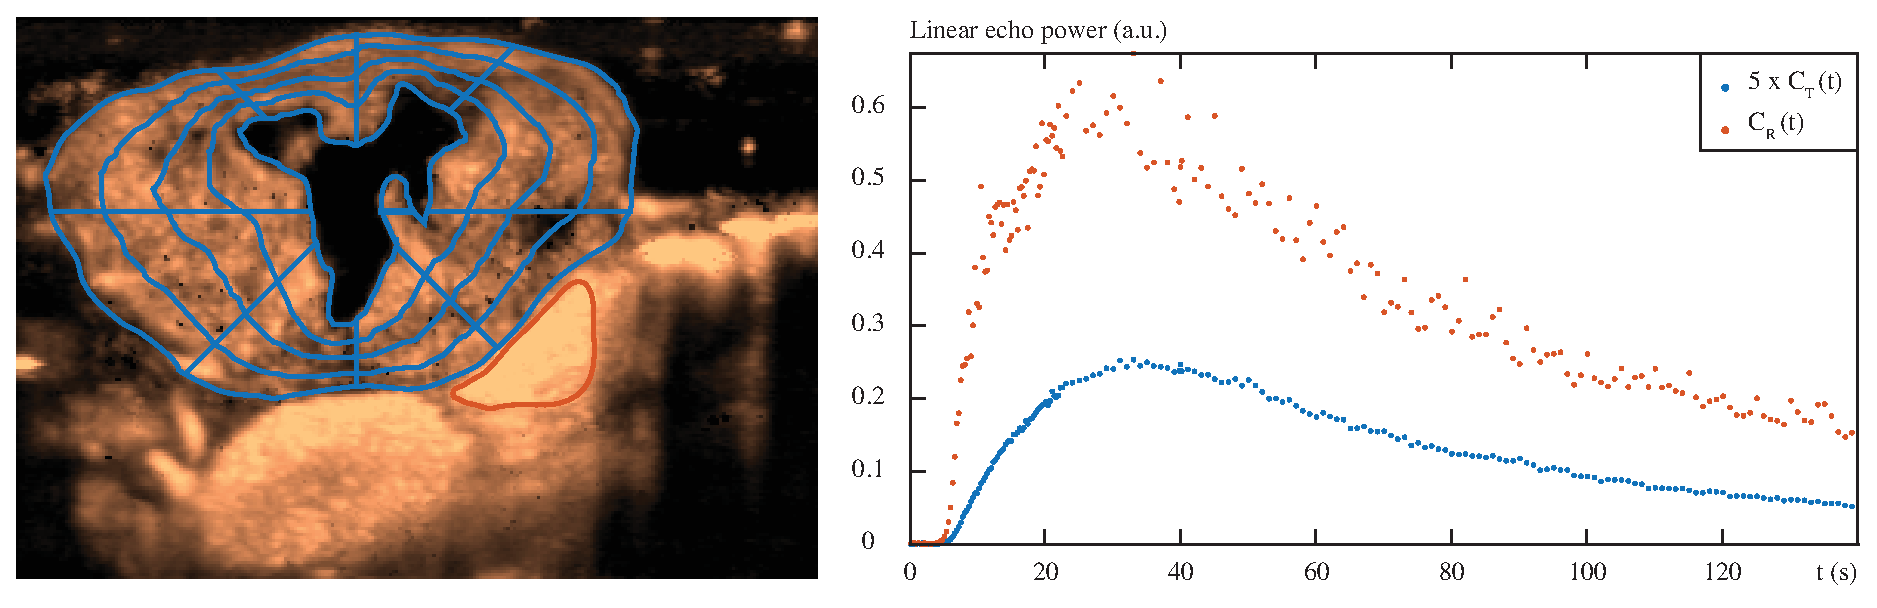
\includegraphics[width=\textwidth]{Ch4_Figure1.eps}
	\caption{Illustration of the data pre-processing steps. Left: The contours of the perfused tumor area have been overlaid on a contrast-enhanced image (in blue color). This area was automatically divided into 4 radial layers and 8 angular sectors as shown by the spiderweb patterns. A RT region (in orange color) was also delineated. Right: Mean TICs associated with the perfused area of the tumor, and the RT.} 
  	\label{fig:Segmentation}
\end{figure*}
\section{Methods}
\subsection{Data pre-processing}
Linear echo-power TICs were calibrated from log-compressed video data using a laboratory-made software.
Both probe and animal motion were assumed negligible for the selected sequences. 

Tumors (hereafter labeled with subscript T) were segmented on the B-Mode images and the non-perfused areas were removed for data analysis.
In order to preserve the signal-to-noise-ratio (SNR) of the TICs while revealing the spatial heterogeneity of the tumor, a regional analysis of the tumor area was performed. 
The perfused tumor region was divided into $N_T = 32$ sub-regions according to 4 radial layers and 8 angular sectors (Figure~\ref{fig:Segmentation}). 
Then mean regional TICs $C_T^i(t)$, for $i=1,...N_T$ were computed. 
As three of the four quantification methods require the selection of a RT region, for each mouse, this RT region (hereafter labeled with subscript R) was chosen to be easily identifiable on the different test-retest studies. 
A muscular region close to the kidney was generally selected, the renal cortex being excluded from the RT region due to the complexity of perfusion patterns observed inside this structure. 

Finally for each sub-region, a time delay parameter, $D_i$, representing the time of arrival of the contrast agent in the considered region, was estimated as follows:
\begin{equation}
D_i = \max_t \frac{\mathrm d^2}{\mathrm dt^2} (C_T^i * W * W),
\end{equation}
where $W$ is an average filter with a fixed width empirically set to 2.0 seconds. 
Using this specific time delay, all regional TICs were registered in time for subsequent analysis.

\subsection{Definition of the four models}
\subsubsection{Log-Normal model (\textbf{LN})}
This method based on the log-normal distribution was recommended by the EFSUMB for quantification of tumor perfusion in clinical studies~\cite{Dietrich:2012kw}.
The TIC inside the $i^{th}$ region of the tumor, $C_T^i(t)$, is fitted according to equation (\ref{eq:LNmodel}):
\begin{equation}
\begin{array}{rcl}
C_T^i(t) &= & \frac{A_T^i}{\sqrt{2 \pi}\sigma_T^i t} \exp \left( - \frac{\left[ \ln(t) - \mu_T^i \right]^2}{2{\sigma_T^i}^2} \right) \textrm{if } t \geq 0,\\ 
&=& \textrm{0 otherwise.}
\end{array}
\label{eq:LNmodel}
\end{equation}
Regional parameters $A_T^i$, $\mu_T^i$, and $\sigma_T^i$  were estimated for each sub-region. 
Semi-quantitative parameters are then derived from the model, including $AUC^i$ and $WIR^i$. These parameters depend, in a non-linear way, on the parameters of the \textbf{LN} model, $A^i$, $\mu^i$, and $\sigma^i$. Relations have been established, both analytically and experimentally, between parameters derived from the \textbf{LN} model and physiological parameters, showing $AUC^i$ is related to blood volume, and $WIR^i$ to blood flow~\cite{Doury:2017fz}.

\subsubsection{Normalized log-normal model (\textbf{rLN})} 
Regional relative parameters: $rAUC^i$ and $rWIR^i$ were derived from the parameters estimated with the (\textbf{LN}) model in the tumor sub-regions ($AUC_T^i$, $WIR_T^i$) and those estimated in the RT region ($AUC_R$, $WIR_R$). 
They were defined as follows:
\begin{equation}
\begin{cases} 
rAUC^i &= AUC_T^i/AUC_R,\\ 
rWIR^i &= WIR_T^i/WIR_R. 
\end{cases}
\end{equation}

\subsubsection{Simple one-compartment model (\textbf{rLin})} 
The resolution of the one-compartment model follows the graphical analysis technique introduced by Patlak et al.~for the quantification of irreversible tracers in PET. 
The method, based on compartmental modeling, estimates blood-related physiological parameters by means of linear regression, assuming the arterial input function (AIF) is known~\cite{Patlak:1983id}.
This linear approach is generalized to reversible tracers~\cite{Logan:1990jg}. 
These approaches have also been adapted to relax the need for blood sampling or AIF measurement and the kinetics inside a RT region was then used (see for instance~\cite{CardenasRodriguez:2013em}).
This resolution was adapted to CEUS data, considering the ultrasound contrast agent is strictly intra-vascular. Considering a one-compartment model to describe flow exchanges inside the tissue, the following equations can be written for each sub-region, $i = 1,\ldots,N_T$:
\begin{equation}
\frac{\mathrm dC_T^i\left(t\right)}{\mathrm dt} = F_T^i.C_A \left(t\right) - \frac{F_T^i}{V_T^i} C_T^i \left(t\right).
\label{eq:Patlak}
\end{equation}
In (\ref{eq:Patlak}) $C_A \left(t\right)$ represents the arterial input function feeding the tissue, while $V_T^i$ stands for the fractional blood volume, and $F_T^i$ for the blood flow in the sub-region $i$.

Considering jointly the TIC inside the RT region and the TICs in the tumor, and assuming a common feeding input for the RT region and the tumor, we have the following set of equations:
\begin{equation}
\left\{ \begin{array}{rcl}
\frac{\mathrm dC_R\left(t\right)}{\mathrm dt} &=& F_R.C_A \left(t\right) - \frac{F_R}{V_R} C_R \left(t\right),\\
\frac{\mathrm dC_T^i\left(t\right)}{\mathrm dt} &=& F_T^i.C_A \left(t\right) - \frac{F_T^i}{V_T^i} C_T^i \left(t\right), \forall i.\\
\end{array}\right.
\label{eq:rLin}
\end{equation}

Rearranging the first equation, $C_A\left(t\right)$ can be isolated and expressed as a function of $C_R\left(t\right)$, and then replaced by its new expression in the $N_T$ following equations, yielding the next system:
\begin{equation}
\left\{ \begin{array}{rcl}
C_A \left(t\right) &=& \frac{1}{F_R} \frac{\mathrm dC_R \left(t\right)}{\mathrm dt} + \frac{1}{V_R} C_R \left(t\right),\\
\frac{\mathrm dC_T^i\left(t\right)}{\mathrm dt} &=& \frac{F_T^i}{F_R} \frac{\mathrm dC_R \left(t\right)}{\mathrm dt} + \frac{F_T^i}{V_R} C_R \left(t\right) - \frac{F_T^i}{V_T^i} C_T^i \left(t\right).
\end{array}\right.
\end{equation}
After integration over time (from 0 to $t$), and definition of the parameters $rF^i = F_T^i/F_R$ , $rV^i = V_T^i/V_R$, and $k_T^i = F_T^i/V_T^i$, the last equations of the system become:
\begin{equation}
C_T^i\left(t\right)=rF^iC_R \left(t\right) + rV^ik_T^i \int_0^t C_R \left(\tau\right)\mathrm d\tau - k_T^i\int_0^t C_T^i \left(\tau\right)\mathrm d\tau.
\label{eq:rLin2}
\end{equation} 
For each sub-region $i$, a sub-system of $N$ linear equations (\ref{eq:rLin2}) is computed, obtained for $N$ successive values of $t$. $N$ is the total number of dynamic frames. Solving this sub-system of $N$ linear equations, the parameters $rF^i$, $rV^i$, and $k_T^i$ can thus be estimated in the least-squares sense. Using this approach, the $N_T$ linear equations corresponding to the different sub-regions are thus solved independently. 

\subsubsection{Regularization of the one-compartment model (\textbf{rLinReg})}
Using the previously described \textbf{rLin} model, $N_T$ different values of $k_R= F_R/V_R$ can be derived, using the estimation of $rF^i$, $rV^i$, and $k_T^i$ and the relation between the four parameters:
\begin{equation}
k_R = \frac{F_R}{F_T^i}\frac{F_T^i}{V_T^i}\frac{V_T^i}{V_R} = \frac{rV^i.k_T^i}{rF^i} \quad \text{for } i = 1,\ldots,N_T.
\end{equation}
As the $k_R$ values do not depend on sub-region $i$, the simple estimation proposed by \textbf{rLin} can introduce some inconsistencies $k_R$  and possible biases in some $rF^i$, $rV^i$, and $k_{T}^i$ values. To solve this issue,
and consider one single value for $k_R$ (whatever the number of sub-regions in the tumor), the regularized approach solves the system of equations  (Eq.~\ref{eq:rLin2}), under the following constraints:
\begin{equation}
\frac{rV^i.k_T^i}{rF^i} = K, \quad \forall i = 1,\ldots,N_T,
\end{equation}
where $K$ is a constant (equal to $k_R$).
The system is solved globally for the $N_T$ sub-regions. Briefly, the value of $k_R$ is successively modified, thus providing a unique least-squares solution for the $3N_T$ parameters ($rF^i$, $rV^i$, and $k_{T}^i$), until the optimization of the fit for the whole set of $N_T$ sub-regions.

\subsection{Data analysis}
For each model, a vector ($\Theta$) of $M$ perfusion parameters ($\theta_m$) was estimated in each tumor sub-region ($i=1,\ldots,32$) of each mouse ($j=1,\ldots,4$) for each repeated acquisition ($k=1,\ldots,4$), providing $512$ results of curve fitting, $\Theta^{ij}_k$, per model. 
The fit quality was assessed quantitatively, using the fraction of modeled information, $FMI$, according to~\cite{Balvay:2005ca}. 

The reproducibility of the perfusion parameters was then deduced for each sub-region of each mouse by computing coefficients of variation $CV(\theta_m)^{ij}$ defined for the four repeated studies, as the ratio between the standard deviation and the mean value $\mu_{m}^{ij}$ of the parameter $(\theta_{m})^{ij}_k$: 
\begin{equation}
{CV(\theta_m)^{ij}} = \frac {\sqrt {\frac{1}{4} {\sum _{k=1}^{4} ((\theta_{m})^{ij}_k- \mu_{m}^{ij})^2}}} {\mu_{m}^{ij}}.
\label{eq:CV}
\end{equation}
Parameters corresponding to poor quality fits ($FMI > 90\% $) were replaced using multivariate imputation by chained equations with the R module \{mice\}~\cite{vanBuuren:2011ica}. This strategy was defined to compute the CV using four values systematically.

Statistical tests were finally applied to compare the CV of the parameters estimated using the four models.
Significant differences in the CV distributions were assessed using the Friedman test and the associated post-hoc analysis for multiple comparisons.  
Distribution means were considered as significantly different when p-values were less than $0.05$.

\section{Results}
\begin{table}[bth]
\begin{center}
\begin{tabular}{lccccc}
\toprule
Model & \textbf{LN} & \textbf{rLN} &\textbf{rLin} & \textbf{rLinReg} \\
\midrule
$FMI$ & 99.3\% & 99.3\%  & 98.8\%  & 98.1\%  \\
$N_{rem}$ & 28  &  28 & 1 & 39 \\
\bottomrule
\end{tabular}
\caption{Median values of $FMI$ obtained for the four models and number of sub-regions $N_{rem}$, out of $512$, for which $FMI <90\%$.}
\label{tab:FMI}
\end{center}
\end{table}

Table~\ref{tab:FMI} shows the median values of the FMI obtained for the four models and the number of regions excluded from further statistical analysis because of bad fit quality. 

\begin{figure}[bth]
  \centering
  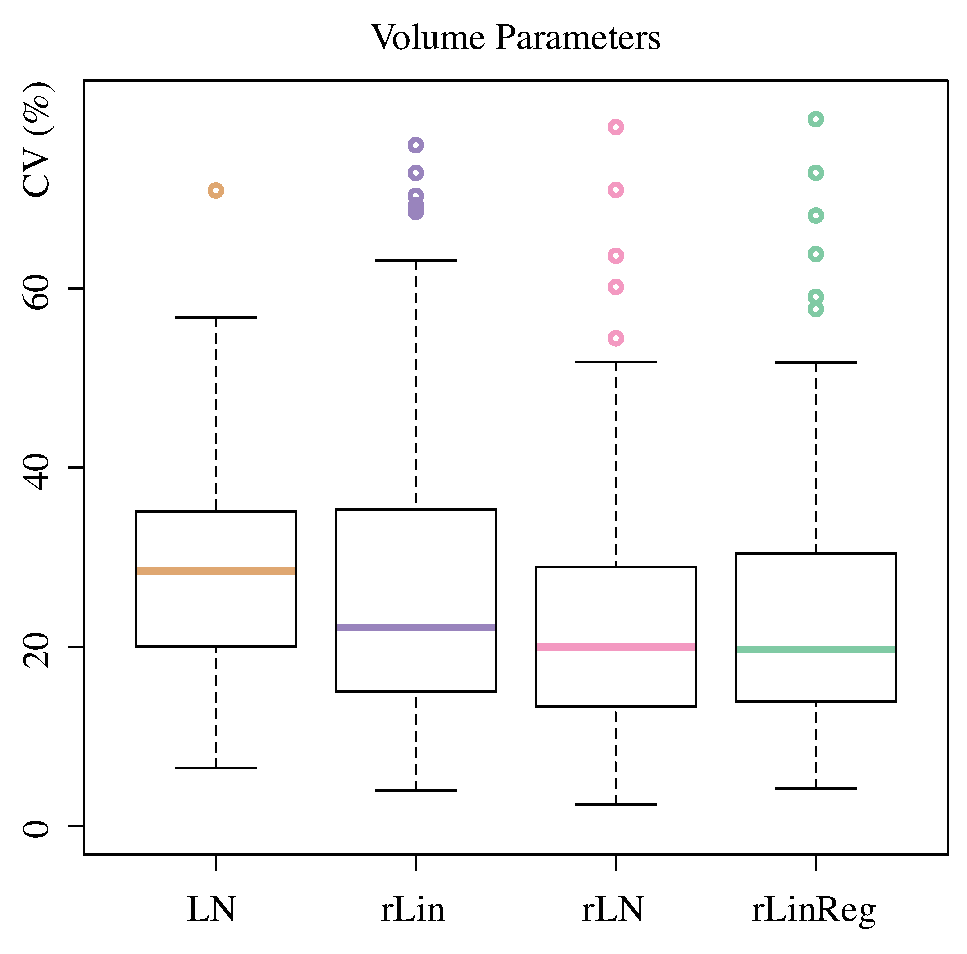
\includegraphics[width=0.49\linewidth]{Ch4_V_CV.eps}
  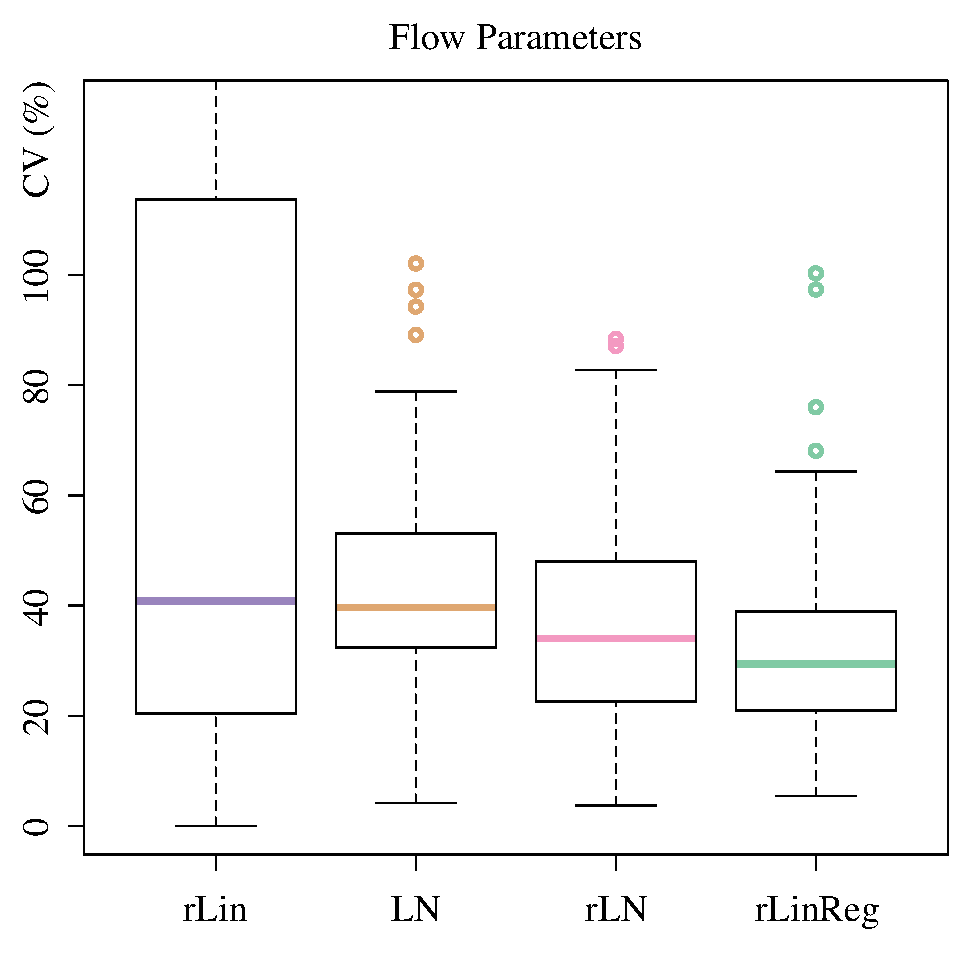
\includegraphics[width=0.49\linewidth]{Ch4_F_CV.eps}
  \caption{Boxplot showing the CV of blood volume  (left) and blood flow (right) estimated with the \textbf{LN}, \textbf{rLN}, \textbf{rLin}, and \textbf{rLinReg} models.}
\label{fig:CV}
\end{figure}

Figure~\ref{fig:CV} displays a boxplot of the $128$ coefficients of variation of blood volume parameters and blood flow parameters obtained for the four models \textbf{LN}, \textbf{rLN}, \textbf{rLin}, and \textbf{rLinReg}. 

\begin{table}
\begin{center}
\begin{tabular}{lcccccc}
\toprule
& \multicolumn{3}{c}{Volume parameters} & \multicolumn{3}{c}{Flow parameters} \\
\cmidrule(l){2-4} \cmidrule(l){5-7}
& \textbf{rLinReg} & \textbf{rLin} & \textbf{rLN} & \textbf{rLinReg} & \textbf{rLin} & \textbf{rLN} \\
\midrule
\textbf{LN} & \textbf{0.001} & 0.1 & \textbf{0.003} & $\mathbf{7 \times 10^{-6}}$ & 0.96 & 0.74 \\
\textbf{rLN} & 0.995 & 0.73 & & $\mathbf{5 \times 10^{-4}}$ & 0.49 \\
\textbf{rLin} & 0.52 & & & $\mathbf{8 \times 10^{-7}}$ \\
\bottomrule
\end{tabular}
\caption{p-values obtained in the post-hoc analysis of the Friedman test. Significant results ($\mathrm p < 0.05$) in bold.} 
\label{tab:pVal}
\end{center}
\end{table}

The p-values obtained after the post-hoc analysis of the Friedman test are shown in Table~\ref{tab:pVal}, significant differences in parameter distributions are emphasized in bold.

In terms of blood volume parameters, the \textbf{LN} model is the most variable with a median value of the coefficient of variation (CV) equal to 28.5\%. 
Using the \textbf{rLin} model, the median CV tends to be lower (22.2\%), however the difference is not statistically significant. 
Models \textbf{rLN} and \textbf{rLinReg} yield significantly more reproducible blood volume parameters than \textbf{LN}, with median CV values of 20.0\% and 19.7\%, respectively. 
For the blood flow parameters, models \textbf{rLin} and \textbf{LN} appear to the most variable parameters with medians of CV equal to 40.8\% and 39.6\%, respectively. 
The \textbf{rLN} model tends to yield lower CV, with a median value of 34.1\%.
Finally the mean CV of blood flow using the \textbf{rLinReg} model is equal to 29.4\%. It is significantly lower than the CV of blood flow obtained with the three other models.

\section{Discussion}
The number of sub-regions was chosen to reveal some spatial heterogeneity in the vascular network of the tumor, while ensuring regions were large enough to guarantee reasonable signal to noise ratios in regional TICs. 
Increasing the number of regions would reveal spatial heterogeneity more finely, at the expense of the accuracy of the estimates.

Both physiological and experimental variations get in the way of accurate quantification and exam comparison, affecting blood circulation, as well as measurements accuracy~\cite{Tang:2011fja}.
The semi-quantitative parameters of the \textbf{LN} model, recommended for tumor quantification, were found highly sensitive to inter-exam changes in our study and resulted in the least reproducible parameters. 
 
When compared to the \textbf{LN} model, the normalized version, the \textbf{rLN} model reduces the variability of parameters. If the reduction of variability for blood flow parameters was not statistically significant, it was significant for blood volume parameters. Thus normalization using a RT region has a real potential to improve exam comparison.

Similarly to the \textbf{rLN} approach, the \textbf{rLin} model uses the RT region, but in addition, it assumes a one-compartment model to describe contrast exchanges between large vessels and micro-vascular areas in tissue.
The first resolution method, which was tested in the present study and proposes to estimate three unknown parameters per sub-region, yields highly variable parameters, especially in terms of blood flow. However, the median CV of blood volume was  reduced when compared to  $AUC$ CV, estimated with the \textbf{LN} model.
This method was implemented in a naive way, resulting in inconsistent values of parameter $k_R$ in the different tumor sub-regions. 

The \textbf{rLinReg} model was built to overcome these inconsistencies, ensuring a single value of $k_R$.
Enforcing a common value of $k_R$ in sub-regions comes down to impose a fixed ratio between the first and second terms of Eq.~\ref{eq:rLin2}.
The number of degrees of freedom was thus reduced. 
The combined use of normalization through a RT region and regularization respects the compartmental modeling paradigm while yielding the most reproducible parameters in our study.

\section{Conclusion}

Using the \textbf{LN} model, derived parameters have high coefficients of variation. 
The positive impact of normalization using a reference tissue region on parameter reproducibility was established. 
The \textbf{rLinReg} approach takes into account the different sub-regions involved in the quantification, yielding a single value of parameter $k_R$ common to all tumor sub-regions. 
In addition, this spatial regularization significantly reduces coefficients of variations of the blood flow parameter and should therefore be preferred to estimate spatially-distributed perfusion parameters.

\clearpage
\appendix
%\addcontentsline{toc}{part}{Appendix}

\chapter*{List of publications}
\addcontentsline{toc}{part}{List of publications}

\section*{Published}
\begin{itemize}
\item Doury M, Dizeux A, De Cesare A, Lucidarme O, Bridal LS, Frouin F, Regularized linear resolution of a one-compartment model to improve the reproducibility of perfusion parameters in CEUS, IEEE International Ultrasonics Symposium (IUS), Tours, France, 2016.
\item Doury M, Dizeux A, De Cesare A, Lucidarme O, Pellot-Barakat C, Bridal LS, Frouin F, Quantification of tumor perfusion using dynamic contrast-enhanced ultrasound: Impact of Mathematical Modeling, Physics in Medicine and Biology, 2017.
\end{itemize}

\section*{In press}
\begin{itemize}
\item Doury M, De Cesare A, Bridal LS, Pellot-Barakat C, Frouin F, Impact of Recirculation in Dynamic Contrast-Enhanced Ultrasound: a Simulation Study, IRBM, 2017.
\end{itemize}

\section*{In writing}
\begin{itemize}
\item Doury M, De Cesare A, Pellot-Barakat C, Bridal LS, Frouin F, Error Sources Affecting Relative Quantification of Dynamic Contrast-Enhanced Ultrasound, Medical Image Analysis
\end{itemize}

\section*{Oral communications}
\begin{itemize}
\item Doury M, Comparison of three modelling approaches in CEUS studies, Dynamics and Control of Tumor Growth Workshop (DYCOTUG), Rouen, France, 2015.
\item Doury M, Dizeux A, De Cesare A, Lucidarme O, Bridal SL, Frouin F, Regularized linear resolution of a one-compartment model to improve the reproducibility of perfusion parameters in CEUS, IEEE International Ultrasonics Symposium (IUS), Tours, France, 2016.
\item Doury M, Bridal LS, Frouin F, How to measure tumor perfusion for exam comparison?, RITS 2017, Lyon, France, 2017.
\end{itemize}

\section*{Posters}
\begin{itemize}
\item Doury M, Dizeux A, Barrois G, Lucidarme O, Bridal L, De Cesare A, Frouin F, Suivi longitudinal en imagerie ultrasonore multimodale pour la caract\'erisation d’un mod\`ele tumoral, Journ\'ees de l’\'Ecole Doctorale Pierre Louis de Sant\'e Publique (ED393), Saint-Malo, France, 2014.
\item Doury M, Dizeux A, Barrois G, Le Guillou-Buffelo D, Coron A, Bridal L, De Cesare A, Frouin F, Local classification of microvascular function based on contrast-enhanced ultrasound data: a feasibility study, Journ\'ees de Recherche en Imagerie et Technologies pour la Sant\'e (RITS), Dourdan, France, 2015.
\item Doury M, Dizeux A, Bridal L, De Cesare A, Frouin F, Impact of three modeling approaches on the reproducibility of perfusion parameters in CEUS studies, Journ\'ees de l’\'Ecole Doctorale Pierre Louis de Sant\'e Publique (ED393), Saint-Malo, France, 2015.
\item Doury M, Dizeux A, De Cesare A, Lucidarme O, Bridal SL, Frouin F, Comparison of three modelling approaches on the reproducibility of perfusion parameters in CEUS studies, International Symposium on Biomedical Imaging: From Nano to Macro (ISBI), Prague, Czech Republic, 2016.
\item Doury M, Dizeux A, De Cesare A, Lucidarme O, Bridal SL, Frouin F, Impact of the modelling approach on the reproducibility of perfusion parameters in CEUS studies, Journ\'ees de l’\'Ecole Doctorale Pierre Louis de Sant\'e Publique (ED393), Saint-Malo, France, 2016.
\item Doury M, De Cesare A, Bridal LS, Frouin F, Impact of Recirculation in Dynamic Contrast Enhanced Ultrasound: A Simulation Study, RITS, Lyon, France, 2017. Prix jeune chercheur SFGBM.
\end{itemize}
% \import{./Body/appb/}{appb.tex}
%\chapter{Bioinformatics and handwriting/speech recognition: unconventional applications of similarity search tools}
\section{Introduction}
	Bioinformatics has benefited immensely from tools and techniques imported
	from other disciplines.  Markov models used for gene--finding have
	their origin in information science, neural networks are imported
	from machine learning, and the countless clustering methods used
	for analyzing microarray data are from a wide variety of fields.

	Sequence alignment tools are no exception to this trend;
	however, within bioinformatics, they have reached
	new levels of speed and sophistication.  Tools,
	such as Blast~\cite{altschul1990basic,altschul1997gapped}
	and FastA~\cite{pearson1998improved}, are used routinely to search
	through a database for sequences (DNA or protein) that are
	similar to a query sequence.  Over the years, these tools have
	been optimized for speed by employing a number of heuristic
	shortcuts to the dynamic programming algorithms on which
	they are based.  Even searches in very large databases,
	such as Swiss--Prot/TrEMBL~\cite{bairoch2000swiss-prot} or
	GenBank~\cite{benson2000genbank}, take only a few seconds
	for queries of small to moderate size.	This is substantially
	faster than the time required for a rigorous Smith--Waterman
	search~\cite{waterman1984efficient}.  In light of the remarkably
	speed and accuracy that characterize these algorithms, it is 
	intriguing to investigate other applications where similarity
	search tools might be of material importance.  In this work, we present two
	alternative applications of these fast sequence alignment tools
	outside the domain of bioinformatics: handwriting recognition and
	speech recognition.

	The dynamic handwriting recognition problem is to recognize
	handwriting from a touch tablet as found on personal
	digital assistants (PDAs), for example Palm Pilots, or tablet
	PCs~\cite{tappert1990thestate}.  These writing tablets sample
	the position of a pen as a function of time to produce a series of
	($x,y$) points that are used by handwriting recognition algorithms to
	determine which character was written.	An excellent review of the
	most common algorithms is available from Plamodon and Srihari, 2000.
	These include feature analysis, curve matching, Markov models, and
	elastic matching, the last of which is based on dynamic programming
	and is related to both Blast and FastA.

	To apply similarity search concepts to the handwriting recognition
	problem, we represented the path of a PDA pen as a protein
	sequence by translating the ($x,y$) points into a string of
	amino acids.  Using the protein representation of handwriting
	samples, we were able to classify unknown samples with FastA. 
	This is analogous to the problem of protein annotation using
	similarity searching: given a protein (a written character)
	of unknown function, we annotated the protein by searching for
	similar sequences (characters with similar ($x,y$) paths).

	We applied the same sequence alignment approach to speech
	recognition.  Automated phone services, security checkpoints,
	and computer dictation software employ some form of speech
	recognition.  Common speech recognition methods include feature
	recognition, neural networks, hidden Markov models, dynamic
	programming~\cite{ney2000progress} and a variety of other statistical
	and signal processing algorithms.  A good review of these techniques
	and more is available from Juang \& Furui, 2000.  For this problem,
	we represented digital speech recordings as sequences of amino
	acids, and used a database of annotated recordings to classify
	unknown recordings.

	In the following section, we describe the data sets used for the
	handwriting recognition and speech recognition problems.  Then,
	we detail how these data were represented using strings of amino
	acids and how we used FastA to annotate unknown samples in four
	handwriting and speech recognition experiments.  We compare our
	results to more traditional methods of handwriting and speech
	recognition and, finally, we discuss ways of improving upon the
	results and extending sequence alignment to other classification
	problems.

		\begin{figure}[t!]
				\centering
				\includegraphics[width=\textwidth]{Body/Images-appc/digits.pdf}
			\caption{Projection of a digit written with
					a PDA stylus into protein space.
					Concatenating the set of
					points gives a protein sequence
					representative of the digit.
					In this case, the sequence is
					\texttt{QYKXVVFMWGSNHANQ}.%
					An alignment of nines from two
					different writers.  The boxes at
					the top show the input from each
					writer and the large grid show the
					superposition of the two handwritten
					digits.  The FastA alignment between
					the protein representations of the
					two digits is shown in the center.
				Two visualizations of the handwriting
				recognition problem.  In both cases the
				$x$ and $y$ axes are divided into 23 parts
				corresponding to the columns and rows in
				an amino acid scoring matrix.  The eight
				sampled points from the digit are cast from
				$x,y$ space into protein space by assigning
				amino acid coordinates to each point.
			}\label{fig:pda}\label{fig:pdaAlign}
		\end{figure}

		\begin{table*}[t!] 
			\centering
			\caption[fooba]{Results for the handwriting and
				speech recognition problems described
				in the text.  For each experiment,
				the misclassification is the percent of
				sequences in the unknown set for which the
				digit or letter was not predicted correctly.}
			\subtable[
				Handwriting recognition results.
			]{\input{Body/Images-appc/table_results1}} \subtable[Speech
				recognition results.
				The second column shows the
				misclassification using the clustering of
				all /ee/ sounding letters as described in the
				text.  ]{ \input{Body/Images-appc/table_results2} }
			\label{table:results2}\label{table:results1}
		\end{table*}


		\begin{table*}[!b]
		\centering
		\caption[Handwriting Alignment Scoring Matrix]{The scoring matrix used for the handwriting
			and speech recognition FastA alignments.
			Each entry of the scoring matrix, $s_{ij}$, is given by $s_{ij}= 10-(|i-j|)$.
			That is, matching amino acids are given 10 ``points'', amino acids
			that are one off are given 9 points, and so on.  This matrix was used
			in place of the default scoring matrix,  Blosum50~\cite{henikoff1992aminoacid},  for FastA.
			The scoring matrix was found heuristically.  Also, a few experiments indicated that the
			alignments are relatively insensitive to permutations about the form of $s_{ij}$ given above.

		} \label{table:matrix}
		\include{Body/Images-appc/table_matrix}
		\end{table*}

		\begin{figure}[ptbh]
		\centering
		\includegraphics[width=\textwidth]{Body/Images-appc/voice.pdf}
		
			%\scalebox{0.80}{
			%	\footnotesize
			%	\input{Body/Images-appc/fig_voiceAlign}
			%	\normalsize
			%}
		\caption[A Voice alignment]{
			An alignment of the spoken--letter ``X'' recorded from two different speakers.
			The plots at the top and bottom are recordings for first and second
			speakers, respectively.  The breakout in the center shows a section of the protein
			projection of each recording and the alignment generated using FastA
			as described in the text.  This example was taken from the first speech
			recognition experiment.  In this case, the bottom recording was the top
			scoring alignment against the top recording.
		}
		\label{fig:voiceAlign}
		\end{figure}

		\begin{figure}[ptbh]
		\centering
		\includegraphics[width=\textwidth]{Body/Images-appc/tree.pdf}
		\caption[A PDA digit]{
			A phylogenetic tree of voice--proteins.
			This tree was created using the
			Phylip~\cite{felsenstein1989phylip} tree drawing
			program from a multiple sequence alignment of
			all 26 voice--proteins from a single speaker.
			The multiple sequence alignment was made using the
			ClustalW~\cite{higgins1992improved} alignment tool,
			with the scoring matrix in Table~\vref{table:matrix}.
			In the tree, similar sounding (homologous) letters
			are grouped near each other.  For example, all the
			letters containing the /ee/ sound [\emph{B, C, D,
			E, G, P, T, V, Z}] are clustered on the left side
			of the tree.
		} \label{fig:tree} \end{figure}



\section{System and Methods}
	\subsection{Handwriting Recognition}
		For our handwriting recognition experiments, we used
		data from Alimoglu and Alpaydin, 1996, available in the
		University of California Irvine repository of machine
		learning databases~\cite{uci1998ucirepository}.  These data
		comprised of 10992 handwritten digits between \emph{0}
		and \emph{9}, written by 44 writers with each writer
		submitting 250 digits (8 samples were discarded by the
		original authors).

		Each digit was written with a stylus pen on a touch tablet,
		which recorded the $x$ and $y$ coordinates of the pen as a
		function of time.  These data were re-sampled such that each
		written digit was represented by a series of eight $(x,y)$
		points, spaced out by a constant arc length over the path of
		the digit.  Then, for each digit, the set of $(x,y)$ points
		were scaled such that the largest axis, usually the $y$ axis,
		ranged from 0 to 1.  By dividing the number line $[0,1]$
		into 23 ``bins'' we translated each of these coordinates
		into a pair of amino acids as shown in Figure~\vref{fig:pda}.
		We concatenated these amino acid pairs to obtain a protein
		sequence representation of each digit: a ``digit--protein.''



		
	\subsection{Speech Recognition}
		For our speech recognition experiments, we used data from
		Deitterich and Bakiri, 1995, %~\cite{dietterich1995solving}
		available in the University of California Irvine repository
		of machine learning databases~\cite{uci1998ucirepository}.
		This data set consisted of 7797 recordings of individuals
		speaking one of the letters \emph{A--Z}.  A total of 150
		speakers each said every letter \emph{A--Z} twice (three
		recordings were discarded by the original authors).
		Then, each recording was processed into a set of 617
		real--valued attributes in the range $[-1,1]$.	A more
		detailed description of the database is available from
		Dietterich \& Bakiri, 1995.%~\cite{dietterich1995solving}.

		By dividing the number line $[-1,1]$ into 23 bins we translated these real numbers into a series
		of amino acids.  For example, the series ``-1.0,-0.55, 0.11, 0.65'' was translated
		to ``{\texttt{AQKY}}''.  We concatenated these amino acids to make a protein representation
		of each recording: a ``voice--protein''.


\section{Results}
	\subsection{Handwriting Recognition}

		We conducted two handwriting recognition experiments.
		In both experiments part of the digit--protein database was assumed to contain a
		``known'' set of digits that was subsequently used to annotate,
		or classify, the remaining ``unknown'' digits.	For our
		first experiment, we used for the known database containing the
		writing of 30 persons (7494 digits) and an unknown database
		with the writing of the remaining 14 persons (3498 digits).
		Using FastA, we searched each sequence from the unknown
		set in the known set and used the top scoring hits to
		annotate the unknown digits.  Searches were carried out
		using the scoring matrix shown in Table~\vref{table:matrix}
		with FastA version 3.4t11 using the default gap open and
		extension penalties, and the following options: \texttt{-p
		-Q -d0 -f-8 -g-1 -H -E1000 -b1}.  An example alignment of
		two handwritten nines from different writers is shown in
		Figure~\vref{fig:pdaAlign}.


		For our second experiment, we used 25\% (2748 digits) of our
		digit--protein database, selected randomly, as the unknown
		set and the remaining 75\% (8244 digits) as our known set.
		Alignments and annotations using FastA were performed as
		in the first experiment.

		The results of the two handwriting recognition
		experiments are shown in Table~\vref{table:results1}.
		In experiment 1, our results are about the same as
		the best k--means clustering results of Alimoglu and
		Alpaydin~\cite{alimoglu1996methods,alimoglu1997combining}.
		This experiment simulates the user--independent
		handwriting recognition problem: the handwriting of one
		group of writers was used to classify digits from a different group.
		In the user--dependent problem, experiment 2, the database
		of known handwritten digits contains samples from all the writers,
		on average.  Thus, for every unknown handwriting sample,
		there is often a close match in the database of known
		samples.  As such, the results of experiment 2 are
		significantly better than those of experiment 1 as shown
		in Table~\vref{table:results1}.



		%In contrast to k--means clustering and other common machine learning techniques for handwriting
		%recognition, there was no explicit training or learning phase of our experiments.  As such, 
		%we included experiment 3, which is a realistic approximation of the recognition problem 
		%on a tablet PC with multiple users.  The results for this experiment are considerably better than
		%experiment 2 because there are relatively more known sequences which can be used for annotating
		%the unknown sequence.

		In experiment 1, the average time for each alignment was
		0.117 seconds per unknown sequence on a 1 gHz Pentium III
		processor.  This is much shorter than the time required to
		write the digits.  Thus sequence alignment could be used
		as a ``real--time'' method for handwriting recognition.
		This high speed, together with the high accuracy for
		user--dependent recognition makes sequence alignment good
		candidate for use on a Tablet PCs, or even PDAs.

	\subsection{Speech Recognition}


		Using the voice--protein database, we conducted two
		experiments, analogous to the two handwriting recognition
		experiments described previously.  First, we used a known
		set consisting of 6238 recordings from 120 speakers and
		an unknown set with 1559 recordings from the remaining 30
		speakers.  Second, we used 25\% (1949 recordings) of the
		voice--protein database, selected randomly, as the unknown
		set and the remaining 75\% (5848 recordings) as the known
		set.  Each of the speech recognition alignments was performed
		using the same scoring matrix and FastA parameters as the
		handwriting recognition experiments.  An example alignment
		of two voice--proteins is shown in Figure~\vref{fig:voiceAlign}.


		The results of the two speech recognition experiments are shown in
		Table~\vref{table:results2}.
		Experiment 1 is compared
		to the best Error Correcting Output Code (ECOC) results of Deitterich
		and Bakiri,
		%~\cite{dietterich1995solving}
		but
		there was no comparison available for experiment 2.	
		The misclassification for experiment 1 was 6.16\%, 
		higher than the ECOC result of 3.27\%.  However, we observed that
		most of the errors were due to rhyming letters, and in particular
		all of the /ee/ sounding characters [\emph{B, C, D, E, G, P, T, V, Z}].
		This indicated that these characters were similar on a sequence level,
		so we constructed a phylogenetic tree of the sequences to study their
		relationship.

	

		A phylogenetic tree of 26 voice--proteins from a single
		speaker is shown in Figure~\vref{fig:tree}.  As the figure
		shows, the protein projections of phonetically similar
		letters tend to be homologous.	Furthermore, letters such
		as \emph{A} and \emph{H}, which have the /ay/ sound at the
		beginning, are more closely related to each other than
		they are to \emph{J} and \emph{K}, which have the /ay/
		sound at the end.  Because the /ee/ sounding letters all
		have /ee/ at the end, they are particularly difficult
		to distinguish from each other.  These letters account
		for a disproportionate majority of the errors in our two
		experiments.  By clustering these letters together such that
		they are considered the same for classification purposes,
		the error in experiment 1 was reduced to 1.09\%.  If the
		original error was evenly distributed between the classes,
		the error would have been reduced only to about 5.5\%.
		This suggests that, although string alignment performs
		poorly for /ee/ sounding characters, it performs well for
		all other characters.


\section{Conclusions}
		This work showed that sequence alignment can be a powerful
		classification tool for problems outside the domain
		of bioinformatics.  In both the handwriting and speech
		recognition problems, we projected real--valued data into
		strings of amino acids and used FastA as a classification
		tool, in a manner analogous to protein annotation.  In the
		case of handwriting recognition, we showed that sequence
		alignment is a viable alternative to traditional methods,
		such as k--means clustering, and is fast enough to be used
		as a real--time recognition method.


		There are many ways to improve upon the results we presented here.
		First, we did not have any explicit training phase for either set of experiments.
		However, there are at least two sequence alignment parameters which can
		be trained: the gap open and extension penalties, and the scoring matrix.
		The optimization of these parameters for protein annotation is well documented
		~\cite{henikoff1993performance,altschul1991amino,henikoff1992aminoacid,dayhoff1979amodel,vogt1995assessment,henikoff2000amino}
		and would be similar for alternative sequence alignment applications such
		as handwriting recognition.  Second, intelligent projection of data
		into strings can greatly improve results.  Here, we used bins of equal
		size to partition the real--valued data into amino acids; however, bins
		of unequal size may improve the resolution between closely related sequences
		and improve classification.  Finally, more customizable sequence alignment tools
		would be very useful.  These tools should take an arbitrary alphabet (Blast
		and FastA are restricted to 23 amino acids) and a user--defined scoring
		matrix (FastA allows user--defined matrices, but Blast does not).

		The potential applications of sequence alignment tools
		outside of bioinformatics are boundless.  Tools such as Blast
		and FastA can be used to quickly classify or search through
		any data that can be projected into a string of characters.
		Of course, these methods will work best with data that is
		of a low dimension.  Our experiments with more complex data
		data, such as color images, suggest that how the data are
		projected into a string is very important with large number
		of dimensions.	However, for simple types of data, such
		as customer purchase histories, black and white images, or
		Internet chat transcripts, we have been able to use sequence
		alignment as a quick and effective classification tool.


%%% This defines the bibliography file (main.bib) and the bibliography style.
%% If you want to create a bibliography file by hand, change the contents of
%% this file to a `thebibliography' environment.  For more information 
%% see section 4.3 of the LaTeX manual.
%\bibliographystyle{plainnat}
\bibliographystyle{abbrvnat}

\clearpage
%\addcontentsline{toc}{chapter}{Bibliography}
\bibliography{References/research-new}

%%\index{structure!protein|see{protein, structure}}

\clearpage
\printindex

\end{document}

